\documentclass[a4paper, 12pt]{article}
\usepackage[spanish,es-tabla]{babel}
\usepackage[utf8]{inputenc}
\makeatletter
\providecommand\IfFormatAtLeastT[2]{}
\providecommand\IfDocumentMetadataT[1]{}
\def\H@refstepcounter#1{%
  \stepcounter{#1}%
  \protected@edef\@currentlabel{\csname p@#1\endcsname\csname the#1\endcsname}%
}
\makeatother
\usepackage[left = 35mm, right = 25mm, top = 25mm, height = 206mm]{geometry}
\usepackage{fancyhdr}
\usepackage{graphicx}
\usepackage{lipsum}
\usepackage[square,numbers]{natbib}
\usepackage[skip=12pt,font=small]{caption}  %Tamaño de la leyenda
\usepackage{subcaption}
\usepackage{amsmath}
\usepackage{afterpage}
\usepackage{titlesec}
\usepackage{array}
\usepackage[table]{xcolor}
\usepackage{listings}
\lstset{
  aboveskip=18pt,
  belowskip=18pt,
  abovecaptionskip=10pt,
  belowcaptionskip=10pt,
  captionpos=t
}
\usepackage{float}
\usepackage{eurosym}
\usepackage{enumitem}
\usepackage{amssymb}
\usepackage{wrapfig}
\usepackage{multirow}
\usepackage{tabularx}
\usepackage{hhline}
\usepackage{url}
\usepackage{eurosym}
\usepackage[titletoc,title]{appendix}
\renewcommand{\appendixtocname}{Apéndices}
\renewcommand{\appendixpagename}{Apéndices}
\usepackage{pdfpages}
\usepackage{pdflscape} %poner pdf horizontal
\usepackage[hidelinks]{hyperref}%para el hiperlink de las secciones
\usepackage[newfloat]{minted}
\usepackage[nottoc]{tocbibind}
\usepackage{glossaries}
\usepackage{diagbox} % Para la línea diagonal en la primera celda de la tabla

\usepackage{tikz} % Diagramas de flujo
\usetikzlibrary{shapes.geometric, arrows, positioning, babel} %Libería de flechas y posicionamiento

\usepackage{datetime}
\newdateformat{monthyeardate}{\monthname, \THEYEAR}


\graphicspath{ {Imagenes/} }


\definecolor{Rojo}{RGB}{255, 87, 51}
\definecolor{Azul}{RGB}{41, 128, 185}
\definecolor{Verde}{RGB}{46, 204, 113}
\definecolor{Naranja}{RGB}{243, 156, 18}
\definecolor{Morado}{RGB}{155, 89, 182}
%\definecolor{Amarillo}{RGB}{241, 196, 15}
\definecolor{Amarillo}{RGB}{253, 253, 150}
\definecolor{Cyan}{RGB}{173, 216, 230}
\definecolor{Rosa}{RGB}{255, 105, 180}
%\definecolor{Rosa}{RGB}{255, 205, 197}
\definecolor{codegray}{rgb}{0.5,0.5,0.5}
%----------------------------------------------------------------------------------------
%	ENCABEZADOS Y PIE DE PAGINA
%----------------------------------------------------------------------------------------

\pagestyle{fancy}
	\fancypagestyle{cuerpo}{
      \fancyfoot{}
      \fancyfoot[L]{Trabajo Final de Grado} %Autor
      \fancyfoot[C]{}
      \fancyfoot[R]{- \thepage \ -}
      \fancyhead{}
      \fancyhead[L]{Trabajo Final de Grado} %Nombre del documento
      \fancyhead[R]{
\includegraphics[height=1.8cm]{Portada/Img/uco_escudo.png}} %Logo Universidad
      \renewcommand{\headrulewidth}{0.4pt}
      \renewcommand{\footrulewidth}{0.4pt}
      \setlength{\headheight}{65pt}
    }
    \fancypagestyle{indice}{
      \fancyfoot{}
      \fancyfoot[L]{\AutorTFG} %Autor
      \fancyfoot[R]{- \thepage \ -} %Asignatura
      \fancyhead{}
      \fancyhead[L]{\leftmark} %Nombre del documento
      \fancyhead[R]{
\includegraphics[height=1.8cm]{Portada/Img/uco_escudo.png}} %Logo
      \renewcommand{\headrulewidth}{0.4pt}
      \renewcommand{\footrulewidth}{0.4pt}
      \setlength{\headheight}{65pt}
      }
      
    \fancypagestyle{plain}{% % <-- this is new
     \fancyfoot{}
      \fancyfoot[L]{Trabajo Final de Grado} %Autor
      \fancyfoot[C]{} %ecc
      \fancyfoot[R]{- \thepage \ -}
      \fancyhead{}
      \fancyhead[L]{\leftmark} %Nombre del documento
      \fancyhead[R]{
\includegraphics[height=1.8cm]{Portada/Img/uco_escudo.png}} %Logo Universidad
      \renewcommand{\headrulewidth}{0.4pt}
      \renewcommand{\footrulewidth}{0.4pt}
      \setlength{\headheight}{65pt}
    }
  
\setcounter{secnumdepth}{4}

% \pagenumbering{empty}

\raggedbottom  % Quita huecos grandes en blanco

\makeatletter
\def\H@refstepcounter#1{%
  \stepcounter{#1}%
  \protected@edef\@currentlabel{\csname p@#1\endcsname\csname the#1\endcsname}%
}
\makeatother

\begin{document}
\setlength{\parskip}{5mm} %Espacio entre párrafos

%%%%%%%%%%%
% PORTADA %
%%%%%%%%%%%
\input{Portada/cover}
\clearpage

% --- PÁGINA DE FIRMA ---
\thispagestyle{empty}
\vspace*{5cm}
\noindent Jacob Pino Moreno, con DNI 51212924H, firmo el presente Trabajo Final de Grado a x de x de 2026.

\vspace{2cm}
\noindent Firma:
\clearpage

% --- RESUMEN ---
\thispagestyle{empty}
\section*{Resumen}
El presente Trabajo Final de Grado (TFG) aborda el diseño, desarrollo e implementación de un sistema domótico local avanzado para la observación y análisis contextual del entorno doméstico. A diferencia de las soluciones comerciales convencionales, que dependen fuertemente de servicios en la nube y comprometen la privacidad, este proyecto propone una arquitectura descentralizada y procesada en el borde (\textit{Edge Computing}) mediante Home Assistant y ESPHome. El sistema integra múltiples sensores (radar de ondas milimétricas, sensores de presencia infrarrojos, temperatura, humedad y luminosidad) distribuidos en nodos estratégicos. Mediante algoritmos de fusión sensorial, la plataforma es capaz de inferir el estado del usuario (estudio, descanso o ausencia) y ejecutar automatizaciones proactivas enfocadas en la mejora del bienestar, la ergonomía y la eficiencia energética, todo ello operando de forma cien por cien local, segura y sin latencia externa.

\vspace{1cm}
\noindent \textbf{Palabras clave:} automatización proactiva, bienestar, domótica local, Edge Computing, ESPHome, fusión sensorial, Home Assistant, IoT, privacidad, radares mmWave.
\clearpage

% --- ABSTRACT ---
\thispagestyle{empty}
\section*{Abstract}
This Undergraduate dissertation presents the design, development, and implementation of an advanced local home automation system for contextual observation and analysis of the domestic environment. Unlike conventional commercial solutions that rely heavily on cloud services and compromise user privacy, this project proposes a decentralized architecture based on Edge Computing using Home Assistant and ESPHome. The system integrates multiple sensors (millimeter-wave radar, infrared presence sensors, temperature, humidity, and light sensors) distributed across strategic nodes. Through sensor fusion algorithms, the platform can infer the user's state (studying, resting, or absent) and execute proactive automations aimed at improving well-being, ergonomics, and energy efficiency, all operating 100\% locally, securely, and with zero external latency.

\vspace{1cm}
\noindent \textbf{Keywords:} Edge Computing, ESPHome, Home Assistant, IoT, local home automation, mmWave radars, privacy, proactive automation, sensor fusion, well-being.
\clearpage

%%%%%%%%%%%%%%%%%%
% INDICE GENERAL %
%%%%%%%%%%%%%%%%%%
\pagenumbering{Roman} % para comenzar la numeracion de paginas en numeros romanos
\pagestyle{indice}
\thispagestyle{indice}
\tableofcontents

\newpage
\renewcommand{\listfigurename}{Índice de ilustraciones}
\listoffigures

\newpage
\section*{Glosario de abreviaturas}
\addcontentsline{toc}{section}{Glosario de abreviaturas}

\noindent
\message{DEBUG: leftmargin=\the\leftmargin, leftskip=\the\leftskip, linewidth=\the\linewidth, textwidth=\the\textwidth, parindent=\the\parindent, oddsidemargin=\the\oddsidemargin}
\renewcommand{\arraystretch}{1.2}
\begin{tabularx}{\textwidth}{@{}p{1.8cm} X@{}}
    \textbf{ADC} & Conversor analógico a digital (\textit{Analog-to-Digital Converter}) \\
    \textbf{API} & Interfaz de programación de aplicaciones (\textit{Application Programming Interface}) \\
    \textbf{BLE} & Bluetooth de bajo consumo (\textit{Bluetooth Low Energy}) \\
    \textbf{CPU} & Unidad central de procesamiento (\textit{Central Processing Unit}) \\
    \textbf{DHT} & Sensor digital de humedad y temperatura (\textit{Digital Humidity and Temperature}) \\
    \textbf{DNS} & Sistema de nombres de dominio (\textit{Domain Name System}) \\
    \textbf{DSP} & Procesador de señal digital (\textit{Digital Signal Processor}) \\
    \textbf{ESP} & Espressif Systems (Familia de microcontroladores IoT) \\
    \textbf{FMCW} & Onda continua modulada en frecuencia (\textit{Frequency Modulated Continuous Wave}) \\
    \textbf{FSM} & Máquina de estados finitos (\textit{Finite State Machine}) \\
    \textbf{GPIO} & Entrada/salida de propósito general (\textit{General Purpose Input/Output}) \\
    \textbf{HA} & Home Assistant (Plataforma domótica de procesamiento local) \\
    \textbf{HTTP} & Protocolo de transferencia de hipertexto (\textit{Hypertext Transfer Protocol}) \\
    \textbf{I2C} & Bus de comunicación serie síncrono (\textit{Inter-Integrated Circuit}) \\
    \textbf{IDE} & Entorno de desarrollo integrado (\textit{Integrated Development Environment}) \\
    \textbf{IoT} & Internet de las cosas (\textit{Internet of Things}) \\
    \textbf{IP} & Protocolo de internet (\textit{Internet Protocol}) \\
    \textbf{ISM} & Banda de radio industrial, científica y médica (\textit{Industrial, Scientific and Medical}) \\
    \textbf{JSON} & Formato de intercambio de datos (\textit{JavaScript Object Notation}) \\
    \textbf{LAN} & Red de área local (\textit{Local Area Network}) \\
    \textbf{LDR} & Fotorresistencia (\textit{Light Dependent Resistor}) \\
    \textbf{LED} & Diodo emisor de luz (\textit{Light Emitting Diode}) \\
    \textbf{LPWAN} & Red de área amplia y bajo consumo (\textit{Low-Power Wide-Area Network}) \\
\end{tabularx}

\newpage

\noindent
\renewcommand{\arraystretch}{1.2}
\begin{tabularx}{\textwidth}{@{}p{1.8cm} X@{}}
    \textbf{MAC} & Dirección de control de acceso al medio (\textit{Media Access Control}) \\
    \textbf{MQTT} & Protocolo de transporte de telemetría por cola de mensajes (\textit{Message Queuing Telemetry Transport}) \\
    \textbf{NAS} & Almacenamiento conectado en red (\textit{Network Attached Storage}) \\
    \textbf{NAT} & Traducción de direcciones de red (\textit{Network Address Translation}) \\
    \textbf{NPU} & Unidad de procesamiento neuronal (\textit{Neural Processing Unit}) \\
    \textbf{OFDMA} & Acceso múltiple por división de frecuencias ortogonales (\textit{Orthogonal Frequency-Division Multiple Access}) \\
    \textbf{OS} & Sistema operativo (\textit{Operating System}) \\
    \textbf{OSI} & Modelo de interconexión de sistemas abiertos (\textit{Open Systems Interconnection}) \\
    \textbf{OTA} & Actualización inalámbrica de firmware (\textit{Over-The-Air}) \\
    \textbf{PIR} & Sensor infrarrojo pasivo (\textit{Passive Infrared Sensor}) \\
    \textbf{PWM} & Modulación por ancho de pulsos (\textit{Pulse Width Modulation}) \\
    \textbf{QR} & Código de respuesta rápida (\textit{Quick Response}) \\
    \textbf{RAM} & Memoria de acceso aleatorio (\textit{Random Access Memory}) \\
    \textbf{RSSI} & Indicador de fuerza de la señal recibida (\textit{Received Signal Strength Indicator}) \\
    \textbf{SBC} & Computador de placa única (\textit{Single Board Computer}) \\
    \textbf{SSD} & Unidad de almacenamiento de estado sólido (\textit{Solid State Drive}) \\
    \textbf{SSH} & Protocolo de acceso remoto seguro (\textit{Secure Shell}) \\
    \textbf{SSL} & Capa de sockets seguros (\textit{Secure Sockets Layer}) \\
    \textbf{SSR} & Relé de estado sólido (\textit{Solid State Relay}) \\
    \textbf{TCP} & Protocolo de control de transmisión (\textit{Transmission Control Protocol}) \\
    \textbf{TLS} & Seguridad de la capa de transporte (\textit{Transport Layer Security}) \\
    \textbf{UI} & Interfaz de usuario (\textit{User Interface}) \\
    \textbf{UML} & Lenguaje unificado de modelado (\textit{Unified Modeling Language}) \\
    \textbf{VPN} & Red privada virtual (\textit{Virtual Private Network}) \\
    \textbf{WAN} & Red de área amplia (\textit{Wide Area Network}) \\
    \textbf{WLAN} & Red local inalámbrica (\textit{Wireless Local Area Network}) \\
    \textbf{WPAN} & Red de área personal inalámbrica (\textit{Wireless Personal Area Network}) \\
    \textbf{YAML} & Formato de serialización declarativo (\textit{YAML Ain't Markup Language}) \\
\end{tabularx}

%---------------------%
%	CUERPO DE TEXTO   %
%---------------------%

\newpage
\newpage

\pagestyle{cuerpo}
\thispagestyle{cuerpo}

\pagenumbering{arabic}

%%%%%%%%%%%%%%%%%%%%%%%%%%%%%%%%%%%%%%%%%%%%%%%%%%%%%%%%%%%%%%%%%%%%%
%                         ESTRUCTURA CONTENIDO                      %
%%%%%%%%%%%%%%%%%%%%%%%%%%%%%%%%%%%%%%%%%%%%%%%%%%%%%%%%%%%%%%%%%%%%%

%------------------%
%   CAPÍTULOS      %
%------------------%

\section{Introducción}
\label{cap:introduccion}

\subsection{Motivación y contexto}
La evolución de la domótica tradicional hacia la inteligencia ambiental (AmI, por sus siglas en inglés) representa un cambio de paradigma en la interacción humano-computadora \cite{ducatel2001ambient}. Históricamente, los sistemas de automatización residencial se han basado en un modelo reactivo, donde el usuario debe accionar comandos explícitos o establecer horarios rígidos para el control del entorno. Sin embargo, la computación sensible al contexto (\textit{context-aware computing}) persigue la creación de espacios capaces de caracterizar la situación del usuario y su entorno de forma transparente, ajustando las variables ambientales sin requerir intervención manual directa \cite{dey2001understanding}.

El despliegue de redes de sensores de bajo coste y el procesamiento local, conocido como \textit{edge computing}, ha facilitado el desarrollo de infraestructuras domóticas que preservan la privacidad del usuario al no depender exclusivamente de procesamientos centralizados en servicios en la nube \cite{shi2016edge}. A pesar de estos avances, la mayoría de implementaciones comerciales de nivel de entrada siguen empleando telemetría binaria básica, como los sensores infrarrojos pasivos (PIR). Estos dispositivos presentan limitaciones severas para determinar la presencia estática prolongada o la posición espacial exacta de un individuo, generando falsos negativos en escenarios de baja movilidad, como el estudio o el descanso \cite{labeodan2015survey}.

El presente proyecto surge ante la necesidad de desarrollar un ecosistema domótico capaz de superar dichas limitaciones volumétricas y lógicas. Mediante la integración de radares de ondas milimétricas (mmWave) \cite{soumya2023mmwave} y técnicas de fusión de sensores, se plantea la construcción de una infraestructura que actúe como un entorno proactivo, capaz de gestionar de manera autónoma la eficiencia energética, la monitorización de rutinas y la seguridad perimetral.

\begin{figure}[htbp]
    \centering
    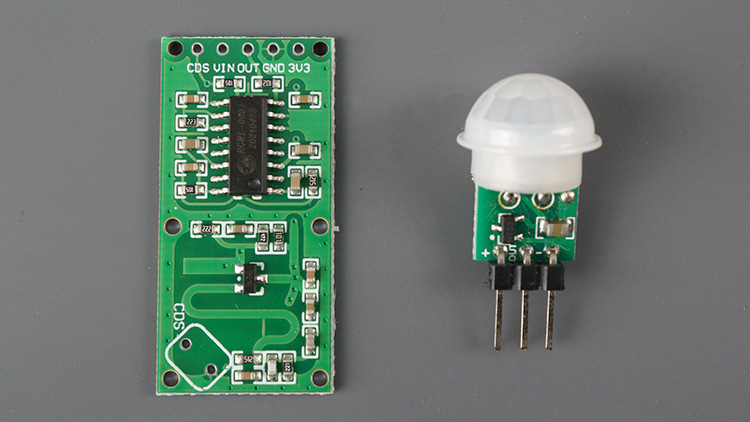
\includegraphics[width=0.6\textwidth]{Img/pir_vs_microwave.png}
    \caption{Comparativa física de componentes: módulo de radar de microondas para detección volumétrica continua (izquierda) frente a sensor infrarrojo pasivo PIR tradicional (derecha).}
    \label{fig:pir_vs_microwave_real}
\end{figure}
\section{Justificación e interés técnico}
El interés técnico de este proyecto se fundamenta en la necesidad de redefinir el paradigma actual de la automatización residencial, trasladando la carga de procesamiento desde infraestructuras dependientes de la nube hacia arquitecturas de ejecución local (\textit{edge computing}). El ecosistema predominante del internet de las cosas (IoT) a nivel de usuario depende de servidores externos para la toma de decisiones, lo que introduce latencias operativas, dependencia de la conectividad a internet y, fundamentalmente, vulnerabilidades críticas respecto a la privacidad y el control de los datos personales \cite{perera2014context}.

Este trabajo justifica la viabilidad e implementación de un sistema basado en inteligencia ambiental (AmI) operado de forma estrictamente local. Al emplear microcontroladores con firmware declarativo y un orquestador centralizado de código abierto en la propia red (como Home Assistant), se garantiza que el procesamiento algorítmico y el almacenamiento de datos no abandonen el entorno físico donde son generados, mitigando los riesgos inherentes al \textit{cloud computing} \cite{shi2016edge}.

En un segundo término, la innovación del proyecto reside en la aplicación práctica de la computación sensible al contexto (\textit{context-aware computing}). La transición de una domótica reactiva a una proactiva exige sistemas capaces de inferir el estado y las necesidades del usuario. Para ello, se aborda la complejidad del modelado del contexto mediante técnicas de fusión de sensores heterogéneos, cruzando variables lumínicas, acústicas y termohigrométricas con telemetría espacial avanzada. Es en este punto donde la integración de radares de ondas milimétricas (FMCW) resulta indispensable. Al sustituir la detección infrarroja tradicional (PIR) por tecnología capaz de registrar micromovimientos respiratorios, se eliminan los falsos negativos prolongados. Esto permite al motor algorítmico asignar estados lógicos de alta fiabilidad (como el estudio o el descanso profundo) sin requerir la interacción directa del individuo \cite{turppa2020vital}.


\subsection{Alcance y limitaciones}

\subsubsection{Alcance del proyecto}
El perímetro operativo de este Trabajo Fin de Grado comprende las siguientes actividades y entregables:
\begin{itemize}
    \item El diseño, ensamblaje y puesta en marcha de dos nodos de hardware distribuidos basados en la plataforma ESP32, equipados con sensórica biométrica y ambiental (FMCW, LDR, transductores climáticos, acústicos, etc.).
    \item La configuración e integración de la red de comunicaciones locales para el transporte de telemetría y comandos de actuación bajo entornos de red local.
    \item El desarrollo de un motor de contexto centralizado capaz de unificar las lecturas heterogéneas mediante lógica de fusión de datos, abstrayendo el comportamiento de la estancia en cuatro estados discretos.
    \item La programación y validación empírica de tres algoritmos de automatización proactiva orientados a la ergonomía visual, la higiene del sueño y la seguridad perimetral contra intrusiones.
\end{itemize}

\subsubsection{Limitaciones del sistema}
El sistema desarrollado presenta restricciones operativas que delimitan su aplicación industrial directa, las cuales se enumeran a continuación:
\begin{itemize}
    \item \textbf{Restricciones volumétricas del radar:} el sensor HLK-LD2410 posee un rango de apertura angular acotado y una distancia máxima de operación de 8 metros, lo que restringe la detección a espacios cerrados de dimensiones medias, requiriendo un estudio de ubicación crítico para evitar zonas ciegas.
    \item \textbf{Vulnerabilidad a interferencias mecánicas:} al operar mediante ondas milimétricas, el radar es susceptible a falsos positivos provocados por elementos en movimiento constante no humano, tales como ventiladores o cortinas desplazadas por corrientes de aire, requiriendo una calibración fina de umbrales por software.
    \item \textbf{Dependencia de la infraestructura de red local:} al prescindir de servicios en la nube para garantizar la privacidad, la operatividad de los nodos y el intercambio de eventos están estrictamente vinculados a la disponibilidad y estabilidad de la red de área local (WLAN) del entorno de pruebas.
    \item \textbf{Vulnerabilidades lógicas delegadas en el perímetro de red:} aunque el procesamiento local elimina los vectores de ataque externos orientados a la interceptación de datos en tránsito hacia la nube, la seguridad global del ecosistema se desplaza y delega por completo en la robustez de los mecanismos de cifrado en la red local. Aunque los microcontroladores empotrados ESP32 presentan restricciones de recursos para gestionar capas de cifrado pesado como TLS/SSL tradicional, la adopción del protocolo Noise (integrado de forma nativa en la API de ESPHome) mitiga este riesgo al cifrar la telemetría en tránsito de extremo a extremo. No obstante, un compromiso de la seguridad de la red inalámbrica doméstica (WLAN) expondría la infraestructura a potenciales ataques de denegación de servicio o suplantación de identidad física.
\end{itemize}

\subsection{Objetivos}

\subsubsection{Objetivo principal}
El objetivo fundamental de este Trabajo Fin de Grado es diseñar, implementar y validar un sistema domótico basado en inteligencia ambiental, capaz de inferir de manera continua el contexto físico y conductual del usuario para automatizar la toma de decisiones relativas al bienestar, la productividad y la seguridad en un entorno residencial, empleando hardware de bajo coste y plataformas de orquestación de código abierto.

\subsubsection{Objetivos específicos}
Para alcanzar la meta principal, se establecen los siguientes objetivos parciales:
\begin{itemize}
    \item \textbf{Diseño de hardware distribuido:} configurar y ensamblar una red de nodos de sensores y actuadores utilizando microcontroladores ESP32, garantizando la cobertura espacial del entorno de pruebas.
    \item \textbf{Implementación de telemetría avanzada:} sustituir la detección de presencia tradicional por telemetría espacial continua, empleando radares de ondas milimétricas (HLK-LD2410) combinados con mediciones lumínicas (LDR) y ambientales.
    \item \textbf{Desarrollo del motor de contexto:} programar un orquestador centralizado que, mediante técnicas de fusión de datos, asigne un estado unívoco a la habitación (ocio, estudio, durmiendo, ausente) en tiempo real.
    \item \textbf{Automatización proactiva y seguridad:} diseñar algoritmos de control lógico para la gestión ergonómica de la iluminación, la evaluación del descanso y el despliegue de un sistema de alarma robusto frente a vulnerabilidades lógicas, como las condiciones de carrera.
    \item \textbf{Validación e integración:} evaluar el comportamiento de la arquitectura propuesta en escenarios de uso real, aplicando redundancias lógicas para verificar la tolerancia a fallos del hardware.
\end{itemize}

\subsection{Metodología empleada}
Para la consecución de los objetivos propuestos, se ha adoptado una metodología de ingeniería basada en el ciclo de vida en V para sistemas empotrados y de IoT, adaptada a desarrollos iterativos \cite{sommerville2011software}. Este enfoque metodológico estructura el proyecto en fases de abstracción descendente seguidas de fases de verificación ascendente, asegurando que cada componente implementado responda directamente a un requisito previamente especificado, como se ilustra gráficamente en la Figura \ref{fig:ciclo_v}.

La metodología se despliega a través de las siguientes fases secuenciales:
\begin{enumerate}
    \item \textbf{Ingeniería de requisitos y restricciones:} definición formal de las necesidades funcionales y de las fronteras físicas del entorno para acotar la selección de componentes.
    \item \textbf{Diseño de la arquitectura e integración de hardware:} fase donde se proyecta la topología de red y se realiza el ensamblaje electrónico, aplicando técnicas de instrumentación en frío y en caliente (uso de multímetros para validación de la caída de potencial en los divisores de tensión de los sensores) para garantizar la estabilidad eléctrica.
    \item \textbf{Desarrollo del firmware y lógica de abstracción:} programación de los microcontroladores mediante abstracciones de hardware declarativas, optimizando los intervalos de actualización y los rangos de atenuación analógica.
    \item \textbf{Orquestación y fusión de datos en el Edge:} implementación de las máquinas de estado y reglas lógicas redundantes en el nodo central para dotar al sistema de tolerancia a fallos ante pérdidas temporales de conectividad o lecturas anómalas de los transductores.
    \item \textbf{Fase de pruebas experimentales y evaluación técnica:} protocolo de validación que abarca desde pruebas unitarias en caja negra hasta pruebas de integración en escenarios reales de uso continuo, analizando la fiabilidad de las transiciones de estado.
\end{enumerate}

    \begin{figure}[htbp]
    \centering
    \begin{tikzpicture}[
        box/.style={draw, rectangle, rounded corners, minimum width=2.5cm, minimum height=0.8cm, align=center, fill=blue!10, font=\scriptsize},
        arrow/.style={thick, -stealth}
    ]
    
    % Explicit coordinates to guarantee it fits the page
    \node[box] (req) at (0, 4) {Ingeniería de\\Requisitos};
    \node[box] (arch) at (2.5, 2.5) {Diseño HW /\\Arquitectura};
    \node[box] (firm) at (5, 1) {Desarrollo\\Firmware};
    
    \node[box] (integ) at (7.5, 2.5) {Integración y\\Orquestación};
    \node[box] (test) at (10, 4) {Pruebas en\\Entorno Real};
    
    % Connections down
    \draw[arrow] (req) |- (arch);
    \draw[arrow] (arch) |- (firm);
    
    % Connections up
    \draw[arrow] (firm) -| (integ);
    \draw[arrow] (integ) -| (test);
    
    % Horizontal verification arrows (dashed)
    \draw[thick, dashed, color=gray, -stealth] (arch) -- node[anchor=south, font=\scriptsize] {Verificación} (integ);
    \draw[thick, dashed, color=gray, -stealth] (req) -- node[anchor=south, font=\scriptsize] {Validación del Sistema} (test);
    
    \end{tikzpicture}
    \caption{Adaptación del modelo del ciclo de vida en V para la metodología de desarrollo de este Trabajo Fin de Grado.}
    \label{fig:ciclo_v}
\end{figure}

\subsection{Estructura de la memoria}
El presente documento se estructura en distintos capítulos organizados para detallar la progresión del proyecto:

El Capítulo 1 introduce el contexto tecnológico, la problemática existente y los objetivos propuestos. El Capítulo 2 presenta la evolución de la domótica y el estado del arte de las tecnologías implicadas. El Capítulo 3 define el problema a resolver y analiza los requisitos del sistema, tanto funcionales como no funcionales. El Capítulo 4 detalla el diseño del sistema, abarcando su arquitectura y modelado lógico. El Capítulo 5 expone la selección e integración de las tecnologías de hardware y software empleadas. El Capítulo 6 describe el plan de implantación y las pruebas realizadas durante el despliegue. El Capítulo 7 realiza una evaluación del sistema desde el punto de vista técnico, económico y de sostenibilidad. El Capítulo 8 recoge el presupuesto del proyecto. El Capítulo 9 presenta los planos y esquemas de la infraestructura. Finalmente, el Capítulo 10 recoge las conclusiones derivadas del trabajo y expone las futuras líneas de investigación. Adicionalmente, se incluyen una serie de anexos con los manuales de usuario y técnicos correspondientes.
\newpage
\section{Contexto y estado del arte}
\label{cap:contexto_estado_arte}

El desarrollo de sistemas inteligentes capaces de interactuar proactivamente con el usuario requiere un análisis exhaustivo de los fundamentos teóricos y tecnológicos que sustentan la inteligencia ambiental. En este capítulo se examina la evolución histórica de la automatización residencial, se analizan críticamente las tecnologías de detección de presencia tradicionales frente a las tecnologías emergentes de radiofrecuencia, y se evalúan los protocolos de comunicación y las arquitecturas de software que posibilitan la gestión centralizada local de redes heterogéneas de internet de las cosas (IoT).

\subsection{Evolución de la domótica y computación ubicua}
La domótica clásica nació ligada a sistemas de automatización, tanto cableados como inalámbricos, de primera generación, orientados principalmente al control remoto y centralizado de la iluminación y la climatización mediante arquitecturas de automatismos rígidos. Estos sistemas primitivos operaban bajo un modelo estrictamente reactivo: el entorno únicamente modificaba su estado tras una acción explícita del usuario a través de interfaces físicas o mandos a distancia.

El cambio paradigmático hacia la automatización contemporánea se fundamenta en los principios de la computación ubicua descritos por Mark Weiser \cite{weiser1991computer}. Este enfoque postula que la tecnología informática debe integrarse de manera orgánica en el entorno cotidiano hasta volverse invisible para el usuario, operando en un segundo plano conceptual. La convergencia de la computación ubicua con los sistemas empotrados de comunicación dio origen al concepto de inteligencia ambiental (AmI) \cite{cook2009ambient}. Un espacio dotado de AmI se caracteriza por tres propiedades fundamentales:
\begin{itemize}
    \item \textbf{Sensibilidad al contexto:} capacidad de adquirir e interpretar telemetría ambiental proveniente de sensores distribuidos para determinar el estado del entorno físico.
    \item \textbf{Autonomía proactiva:} facultad de ejecutar acciones de control predictivas basadas en las inferencias contextuales, eliminando la necesidad de comandos manuales.
    \item \textbf{Interacción transparente:} el usuario se sitúa en el centro del sistema, experimentando modificaciones adaptativas en el entorno (ajustes lumínicos, térmicos o de seguridad) sin percibir la infraestructura tecnológica subyacente.
\end{itemize}

En las arquitecturas comerciales típicas de la última década, la inteligencia ambiental se ha supeditado a plataformas de computación en la nube (\textit{cloud computing}). Sin embargo, la necesidad de reducir los tiempos de latencia en la toma de decisiones, optimizar el uso del ancho de banda y garantizar la confidencialidad de la información ha impulsado la adopción del paradigma de computación en el extremo (\textit{edge computing}) \cite{shi2016edge}. En este modelo local, la adquisición, el filtrado algorítmico y la fusión de datos se ejecutan en las fronteras de la red interna, dotando al sistema de autonomía operativa frente a desconexiones de la red externa, como se contrapone gráficamente en la Figura \ref{fig:edge_vs_cloud}.

\begin{figure}[H]
    \centering
    \begin{tikzpicture}[
        cloud/.style={draw, ellipse, minimum width=3cm, minimum height=1.5cm, align=center, fill=blue!5, font=\scriptsize},
        local/.style={draw, rectangle, rounded corners, minimum width=3.5cm, minimum height=4cm, align=center, fill=green!5, dashed},
        device/.style={draw, rectangle, rounded corners, minimum width=2.2cm, minimum height=0.8cm, align=center, fill=white, font=\scriptsize},
        arrow/.style={thick, stealth-stealth}
    ]
    
    % Cloud Architecture
    \node[cloud] (internet) at (0, 5) {Servidor\\Cloud};
    \node[local] (home1) at (0, 1.5) {};
    \node[above=0.1cm of home1, font=\scriptsize\bfseries] {Red Local};
    \node[device] (sensor1) at (0, 1) {Sensores /\\Actuadores};
    
    \draw[arrow, red] (sensor1) -- node[anchor=west, font=\scriptsize, align=left] {Alta latencia\\Dependencia} (internet);
    
    % Edge Architecture
    \node[local] (home2) at (6, 1.5) {};
    \node[above=0.1cm of home2, font=\scriptsize\bfseries] {Red Local (Aislada)};
    \node[device] (sensor2) at (6, 0.2) {Sensores /\\Actuadores};
    \node[device, fill=blue!10] (edge) at (6, 2.3) {Servidor central\\Edge};
    
    \draw[arrow, green!50!black] (sensor2) -- node[anchor=west, font=\scriptsize, align=left] {Baja latencia\\Privacidad} (edge);
    
    \end{tikzpicture}
    \caption{Comparativa arquitectónica: dependencia de la nube frente a procesamiento local (\textit{edge computing}).}
    \label{fig:edge_vs_cloud}
\end{figure}

\begin{figure}[H]
    \centering
    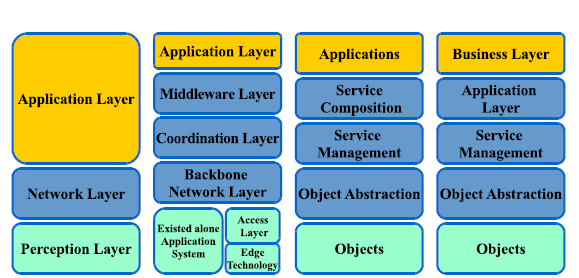
\includegraphics[width=0.75\textwidth]{Img/diagrama_capas.png}
    \caption{Arquitectura en capas característica de los ecosistemas IoT: capa de percepción (sensores), red (WLAN) y aplicación \cite{al2015internet}.}
    \label{fig:diagrama_capas}
\end{figure}

\subsection{Tecnologías de detección de presencia y sus limitaciones}
La correcta inferencia del contexto en un espacio inteligente está vinculada a la fiabilidad de la telemetría de presencia humana. Los sistemas tradicionales han dependido históricamente de transductores binarios de bajo coste, cuyas limitaciones físicas condicionan la estabilidad de las automatizaciones complejas.

\subsubsection{Sensores infrarrojos pasivos (PIR)}
Los dispositivos PIR operan mediante la captación de las variaciones de radiación térmica en el espectro infrarrojo dentro de su campo de visión. El elemento sensor, usualmente piroeléctrico, está segmentado en ranuras diferenciales cubiertas por una lente de Fresnel que enfoca la energía infrarroja. Cuando un cuerpo con una temperatura diferencial respecto al fondo cruza estas ranuras, el transductor genera una fluctuación de tensión que el circuito integrado interpreta como movimiento \cite{labeodan2015survey}.

Esta naturaleza física introduce dos limitaciones severas:
\begin{itemize}
    \item \textbf{Incapacidad de detección estática:} si el sujeto permanece inmóvil (por ejemplo, durante la lectura, el trabajo en escritorio o el sueño), la radiación térmica proyectada sobre el sensor piroeléctrico se vuelve constante, anulando la variación de tensión. Esto genera falsos negativos que interrumpen de forma anómala las automatizaciones.
    \item \textbf{Sensibilidad a gradientes térmicos:} al depender de la temperatura diferencial, los sensores PIR son vulnerables a falsos positivos provocados por corrientes de aire caliente, radiación solar directa sobre superficies interiores o el encendido automático de sistemas de climatización por convección.
\end{itemize}

\subsubsection{Sensores ultrasonidos}
Los sensores acústicos de presencia emiten ráfagas de ondas ultrasónicas de alta frecuencia (típicamente entre 30 kHz y 40 kHz) y miden el tiempo de vuelo (ToF) del eco reflejado o evalúan el desplazamiento de frecuencia provocado por el efecto Doppler al impactar sobre un objeto en movimiento. Aunque superan a los sensores PIR en la detección de movimientos axiales sutiles y no requieren línea de visión directa estricta, presentan una alta vulnerabilidad a interferencias acústicas ambientales, ruidos de conmutación y oscilaciones mecánicas de baja frecuencia generadas por electrodomésticos o tráfico exterior \cite{labeodan2015survey}.

\subsection{Fundamentos del radar de ondas milimétricas (mmWave)}
Para superar la naturaleza puramente binaria de los sensores convencionales, la inteligencia ambiental integrada en el perímetro residencial recurre a sistemas de radar de onda continua modulada en frecuencia (FMCW, por sus siglas en inglés) que operan en el espectro de las microondas de alta frecuencia, específicamente en la banda de 24 GHz \cite{soumya2023mmwave}. Aunque esta banda pertenece técnicamente al espectro de microondas (SHF), comercial e industrialmente suele catalogarse dentro de las tecnologías de ondas milimétricas (mmWave) por su principio de funcionamiento y el reducido tamaño de sus antenas integradas.

El principio de operación de un radar FMCW se basa en la emisión continua de una señal electromagnética cuya frecuencia varía linealmente en el tiempo siguiendo un patrón de rampa o \textit{chirp}. La señal reflejada por los obstáculos en el entorno es captada por la antena receptora del dispositivo. Debido al tiempo de propagación de la onda, existe un desfase temporal entre la señal emitida y la recibida en un instante dado, lo que genera una diferencia de frecuencia medible denominada frecuencia intermedia o de batido ($f_b$) \cite{rao2017introduction}.

El procesamiento analógico y digital de la señal intermedia en el propio microcontrolador del radar se ejecuta mediante la transformada rápida de Fourier (FFT). Este análisis espectral permite discretizar el espacio físico en celdas volumétricas o compuertas de distancia (\textit{range gates}), tal como se modela matemáticamente en la Ecuación \ref{eq:radar_range}:

\begin{equation}
\label{eq:radar_range}
R = \frac{c \cdot f_b \cdot T_c}{2 \cdot B}
\end{equation}

Donde $c$ representa la velocidad de la luz, $T_c$ es la duración del periodo de la rampa de frecuencia, y $B$ corresponde al ancho de banda de la modulación aplicada. 

\begin{figure}[H]
    \centering
    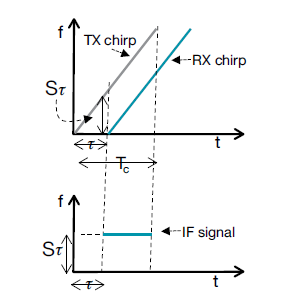
\includegraphics[width=0.45\textwidth]{Img/grafica_chirp.png}
    \caption{Representación en el dominio tiempo-frecuencia de las señales transmitidas (Tx) y recibidas (Rx) en un radar FMCW, ilustrando el retardo temporal $\tau$ y la frecuencia intermedia o de batido resultante \cite{rao2017introduction}.}
    \label{fig:grafica_chirp}
\end{figure}

Mediante la evaluación continua del desfase de fase de los ecos en compuertas de distancia milimétricas, los radares FMCW modernos, como el modelo HLK-LD2410, poseen la resolución necesaria para registrar variaciones submilimétricas en la superficie del cuerpo humano. Esta capacidad analítica faculta al sensor para detectar de manera ininterrumpida los movimientos torácicos asociados a la respiración y los micromovimientos vasculares periféricos, manteniendo el estado de presencia activo incluso si el usuario se encuentra en reposo absoluto o durmiendo, eliminando de raíz los falsos negativos inherentes a la sensórica piroeléctrica \cite{turppa2020vital} (véase la Figura \ref{fig:pir_vs_mmwave}).

\begin{figure}[H]
    \centering
    \begin{tikzpicture}
    
    % PIR Sensor
    \begin{scope}[shift={(0,0)}]
        % Draw cone first (background)
        \fill[red!20, opacity=0.5] (0,2.75) -- (-1.5,0) arc(180:360:1.5 and 0.5) -- cycle;
        \draw[red, dashed] (0,2.75) -- (-1.5,0);
        \draw[red, dashed] (0,2.75) -- (1.5,0);
        
        % Draw sensor box on top
        \node[draw, rectangle, fill=gray!20, minimum width=1cm, minimum height=0.5cm, font=\scriptsize] (pir) at (0,3) {PIR};
        
        \node[font=\scriptsize, align=center] at (0,-1) {Detección binaria\\Zonas ciegas en estático};
        
        % Person
        \fill[black] (0.5,0.5) circle (0.15); % head
        \draw[thick] (0.5,0.35) -- (0.5,-0.2); % body
        \node[font=\scriptsize, red] at (0.5, 0.9) {Falso negativo};
    \end{scope}
    
    % mmWave Sensor
    \begin{scope}[shift={(6,0)}]
        % Draw cone first (background)
        \fill[green!20, opacity=0.5] (0,2.75) -- (-2,0) arc(180:360:2 and 0.5) -- cycle;
        \draw[green!50!black, dashed] (0,2.75) -- (-2,0);
        \draw[green!50!black, dashed] (0,2.75) -- (2,0);
        
        % Draw sensor box on top
        \node[draw, rectangle, fill=gray!20, minimum width=1cm, minimum height=0.5cm, font=\scriptsize] (mmw) at (0,3) {mmWave};
        
        % Waves
        \draw[green!50!black] (0,2.4) arc(90:135:0.5);
        \draw[green!50!black] (0,2.2) arc(90:135:0.7);
        \draw[green!50!black] (0,2.0) arc(90:135:0.9);
        
        \node[font=\scriptsize, align=center] at (0,-1) {Detección continua\\Resolución submilimétrica};
        
        % Person
        \fill[black] (0.5,0.5) circle (0.15); % head
        \draw[thick] (0.5,0.35) -- (0.5,-0.2); % body
        
        % Breathing arrows
        \draw[blue, -stealth] (0.2, 0.3) -- (0.0,0.3);
        \draw[blue, -stealth] (0.8, 0.3) -- (1.0,0.3);
        \node[font=\tiny, blue, anchor=west] at (1.05, 0.3) {Respiración};
    \end{scope}
    
    \end{tikzpicture}
    \caption{Representación conceptual de las limitaciones volumétricas de los sensores PIR tradicionales frente a la detección continua de micromovimientos de los radares mmWave.}
    \label{fig:pir_vs_mmwave}
\end{figure}

\subsection{Protocolos de comunicación IoT}
La integración de nodos distribuidos heterogéneos dentro de una infraestructura local requiere el análisis de los protocolos de transporte y las capas de enlace físico para garantizar la baja latencia y la inmunidad al ruido electromagnético residencial.

\subsubsection{Comparativa de tecnologías inalámbricas}
Las tecnologías de red aplicadas al ámbito del IoT se segmentan principalmente por su alcance, ancho de banda y consumo energético. Las redes WAN de baja potencia (LPWAN), como LoRaWAN, destacan por su gran alcance kilométrico y alta penetración en estructuras densas, propiedades críticas en sistemas de monitorización industrial distribuidos o control de aparcamientos urbanos \cite{mekki2019comparative}. No obstante, sus severas restricciones en la tasa de transferencia de datos y los ciclos de trabajo limitados (\textit{duty cycle}) invalidan su uso para telemetría domótica en tiempo real, donde se requiere el envío constante de flujos analógicos por segundo.

Para entornos domésticos confinados, los protocolos de red en malla basados en el estándar IEEE 802.15.4, como Zigbee, ofrecen un balance óptimo entre consumo y direccionamiento de nodos. Sin embargo, su integración requiere el despliegue de pasarelas específicas de traducción de protocolos. Por este motivo, para el diseño de nodos de instrumentación continua con alimentación permanente, el uso del estándar IEEE 802.11b/g/n (Wi-Fi) sobre la banda de 2.4 GHz resulta el más eficiente. Proporciona una infraestructura de red local preexistente con un ancho de banda elevado que asimila las ráfagas de datos analógicos de los microcontroladores sin introducir cuellos de botella lógicos.

\begin{figure}[H]
    \centering
    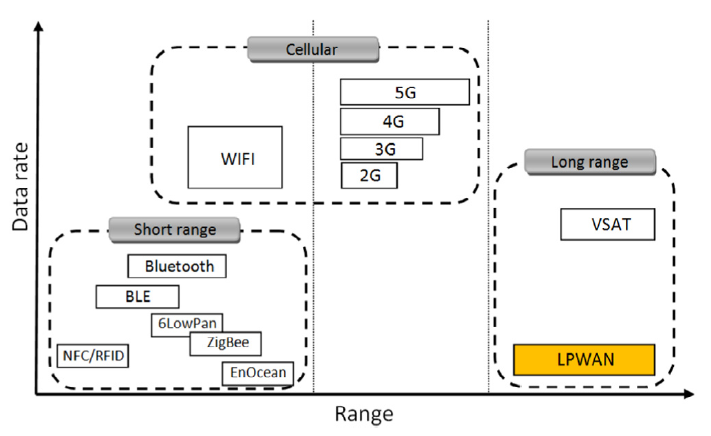
\includegraphics[width=0.7\textwidth]{Img/grafica_protocolos.png}
    \caption{Comparativa de tecnologías inalámbricas para ecosistemas IoT en función de su tasa de transferencia de datos frente a su alcance efectivo \cite{mekki2019comparative}.}
    \label{fig:grafica_protocolos}
\end{figure}

\subsubsection{El protocolo de transporte MQTT}
Sobre la capa de transporte TCP/IP de la red Wi-Fi, el protocolo de mensajería MQ Telemetry Transport (MQTT) se establece como el estándar de facto para arquitecturas perimetrales eficientes. MQTT opera bajo un modelo de publicación/suscripción desacoplado mediado por un agente central o \textit{broker} \cite{al2015internet}, tal y como se esquematiza en la Figura \ref{fig:mqtt_pubsub}.

\begin{figure}[H]
    \centering
    \begin{tikzpicture}[
        broker/.style={draw, circle, minimum size=2cm, align=center, fill=blue!10, font=\scriptsize},
        nodebox/.style={draw, rectangle, rounded corners, minimum width=2.5cm, minimum height=1.2cm, align=center, fill=gray!10, font=\scriptsize},
        arrow/.style={thick, -stealth}
    ]
    
    \node[nodebox] (pub) at (0,0) {ESP32\\(Publisher)};
    \node[broker] (broker) at (5,0) {Broker\\MQTT};
    \node[nodebox] (sub) at (10,0) {Actuador\\(Subscriber)};
    
    \draw[arrow] (pub) -- node[anchor=south, font=\scriptsize] {Publica} node[anchor=north, font=\tiny] {/casa/salon/presencia} (broker);
    \draw[arrow] (broker) -- node[anchor=south, font=\scriptsize] {Notifica} node[anchor=north, font=\tiny] {/casa/salon/presencia} (sub);
    
    \end{tikzpicture}
    \caption{Arquitectura de publicación y suscripción del protocolo MQTT.}
    \label{fig:mqtt_pubsub}
\end{figure}

Frente a protocolos síncronos pesados (como HTTP\slash REST), MQTT ofrece ventajas esenciales para el proyecto:
\begin{itemize}
    \item \textbf{Reducido sobrecoste de protocolo (\textit{overhead}):} la cabecera fija del protocolo es de únicamente 2 bytes, reduciendo el consumo de ancho de banda y los tiempos de serialización en procesadores limitados como el ESP32.
    \item \textbf{Gestión de la calidad de servicio (QoS):} permite parametrizar el nivel de entrega de los mensajes (QoS 0, QoS 1 o QoS 2), asegurando la llegada de eventos críticos relativos a la seguridad perimetral frente a telemetrías ambientales repetitivas.
    \item \textbf{Mecanismo de testamento (\textit{Last Will and Testament}):} permite al \textit{broker} notificar de forma proactiva y automática la desconexión abrupta de un nodo sensor por fallo eléctrico o pérdida de Wi-Fi, habilitando la ejecución inmediata de rutinas de contingencia en el servidor central local.
\end{itemize}

\subsection{Soluciones comerciales y antecedentes}
El mercado actual de consumo ofrece una amplia gama de ecosistemas domóticos propietarios desarrollados por corporaciones tecnológicas internacionales. Plataformas basadas en los ecosistemas de Tuya/Smart Life, Google Home o Philips Hue proporcionan interfaces de usuario pulidas y compatibilidad simplificada mediante el modelo \textit{Plug-and-Play}. Sin embargo, un análisis de ingeniería revela deficiencias estructurales en estas soluciones:

\begin{itemize}
    \item \textbf{Aislamiento en silos tecnológicos:} los fabricantes tienden a restringir la interoperabilidad nativa, forzando al usuario a depender de pasarelas de traducción propietarias y aplicaciones de software independientes que complican la unificación de datos.
    \item \textbf{Dependencia de la nube:} la lógica de conmutación y la ejecución de las automatizaciones de estas soluciones comerciales se procesan en servidores remotos. Si la conexión a internet del hogar se degrada o el servidor del proveedor experimenta una interrupción del servicio, el entorno pierde por completo sus capacidades autónomas.
    \item \textbf{Monetización e intrusión en la privacidad:} el almacenamiento masivo de históricos de presencia, hábitos horarios y perfiles acústicos en infraestructuras externas plantea serios dilemas éticos y legales bajo normativas de protección de datos, al delegar la custodia de información sensible a terceros cuyos modelos de negocio suelen incluir la explotación analítica de datos agregados \cite{perera2014context}.
\end{itemize}

Frente a estos antecedentes comerciales, las arquitecturas de código abierto de integración local como Home Assistant y ESPHome plantean una alternativa sólida. Permiten la unificación de hardware heterogéneo bajo una capa de abstracción común operada de forma local, devolviendo el control operativo y la privacidad absoluta de los datos al perímetro de la vivienda.

Establecido el estado del arte y justificadas las ventajas del procesamiento local y la sensórica avanzada, el siguiente capítulo abordará la definición formal del problema, detallando los requisitos funcionales y no funcionales que guiarán el diseño y desarrollo de la solución propuesta.
\newpage
\section{Definición del problema y análisis de requisitos}
\label{cap:analisis_requisitos}

La ingeniería de requisitos constituye una fase crítica en el ciclo de vida del desarrollo de sistemas, estableciendo el marco de referencia técnico que guiará el diseño y la implementación. En este capítulo se formaliza la especificación del sistema propuesto, delimitando las restricciones operativas, definiendo los actores involucrados y detallando los requisitos funcionales y no funcionales bajo directrices estandarizadas de ingeniería de software \cite{iso29148}.

\subsection{Restricciones y factores limitantes}
El desarrollo e implantación del prototipo están sujetos a un conjunto de restricciones físicas, tecnológicas y temporales que condicionan la arquitectura final:
\begin{itemize}
    \item \textbf{Restricciones de conectividad y latencia:} el sistema opera sobre una red local aislada para garantizar la resiliencia frente a caídas del servicio de Internet (arquitectura \textit{offline-first}). Esto exige que el servidor central y los sensores compartan el mismo dominio de difusión (dominio de \textit{broadcast}) y estén sometidos a una estricta política de red.
    \item \textbf{Restricciones ambientales y volumétricas:} la fiabilidad de la telemetría espacial está supeditada a la geometría de la habitación y a la existencia de línea de visión electromagnética directa entre el radar de ondas milimétricas y los sujetos, limitando las posiciones de instalación viables para evitar zonas de sombra acústica.

    \item \textbf{Restricciones de hardware y procesamiento:} la gestión centralizada central se ejecuta sobre un microordenador Raspberry Pi 4 de recursos finitos. Esto impone una limitación directa sobre la complejidad computacional algorítmica y exige un control estricto sobre el uso de la memoria RAM y el desgaste de la unidad de almacenamiento.
    \item \textbf{Restricciones de infraestructura de red:} el sistema exige cobertura ininterrumpida de red inalámbrica IEEE 802.11 (Wi-Fi) en la banda de 2.4 GHz para la transmisión de la telemetría a través de la API local de los nodos distribuidos, requiriendo un nivel de señal (RSSI) estable para evitar la pérdida de eventos lógicos.
\end{itemize}

\begin{figure}[H]
    \centering
    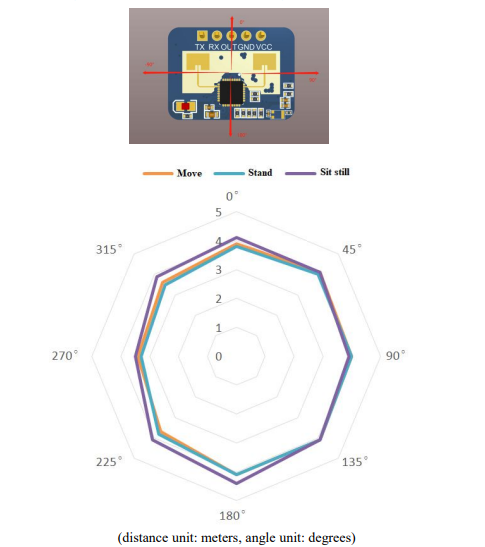
\includegraphics[width=0.7\textwidth]{Img/diagrama_rango.png}
    \caption{Campo de visión volumétrica del sensor FMCW. Adaptado de \cite{datasheetHLKLD2410}.}
    \label{fig:campo_vision_radar}
\end{figure}

\subsection{Identificación de actores del sistema}
Para el modelado lógico de los casos de uso, se identifican los siguientes actores que interactúan de forma directa o indirecta con la infraestructura:
\begin{itemize}
    \item \textbf{Usuario habitual:} actor principal y pasivo. Representa a la persona física que habita el entorno monitorizado. Su interacción consiste en realizar rutinas cotidianas (estudiar, dormir, salir) sin requerir la emisión de comandos explícitos al sistema.
    \item \textbf{Administrador del sistema:} actor activo con privilegios elevados. Encargado del mantenimiento de la infraestructura, el acceso al panel de control analítico, la calibración de los umbrales de sensibilidad de los sensores y la auditoría de los registros de ejecución.
    \item \textbf{Motor de contexto (actor lógico):} entidad de software autónoma que procesa la telemetría entrante, ejecuta los algoritmos de fusión de datos y emite las órdenes de actuación sobre el entorno físico.
\end{itemize}

\begin{figure}[H]
    \centering
    
\begin{tikzpicture}[
        actor/.style={circle, draw=black!80, fill=blue!10, thick, minimum size=1.2cm, align=center, font=\small\sffamily},
        system/.style={rectangle, draw=red!80, fill=white, thick, minimum width=6.5cm, minimum height=6cm, rounded corners},
        usecase/.style={ellipse, draw=black!80, fill=yellow!20, thick, minimum width=3.5cm, minimum height=1.2cm, align=center, font=\footnotesize\sffamily},
        arrow/.style={->, >=stealth, thick, color=black!70}
    ]
        % Sistema
        \node[system] (sys) at (0,0) {};
        \node[anchor=north, font=\bfseries] at (sys.north) {Sistema Domótico};

        % Casos de uso
        \node[usecase] (cu1) at (0, 1.8) {Calibración y\\Auditoría};
        \node[usecase] (cu2) at (0, 0) {Generación de\\Telemetría};
        \node[usecase] (cu3) at (0, -1.8) {Inferencia de\\Estados y Actuación};

        % Actores
        \node[actor] (admin) at (-4.5, 1.8) {Admin.};
        \node[actor] (user) at (-4.5, -0.5) {Usuario\\habitual};
        \node[actor, fill=green!10] (engine) at (4.5, -1.5) {Motor de\\Contexto};

        % Conexiones
        \draw[arrow] (admin) -- (cu1);
        \draw[arrow] (user) -- (cu2);
        \draw[arrow] (engine) -- (cu3);
        
        \draw[arrow, dashed] (cu2) -- (engine);
    \end{tikzpicture}
    \caption{Diagrama de casos de uso y actores del sistema.}
    \label{fig:casos_uso_actores}
\end{figure}

\subsection{Requisitos funcionales (RF)}
Los requisitos funcionales describen las operaciones y comportamientos específicos que el sistema debe ser capaz de ejecutar en su entorno de producción.
\begin{itemize}
    \item \textbf{RF-01: Monitorización espacial continua.} El sistema debe detectar la ocupación volumétrica con resolución submilimétrica, diferenciando de manera inequívoca los estados de movimiento dinámico y reposo biométrico absoluto.
    \item \textbf{RF-02: Adquisición de telemetría ambiental.} El sistema debe registrar variables de luminosidad ambiental e índices termohigrométricos para nutrir la matriz de contexto.
    \item \textbf{RF-03: Inferencia algorítmica de estados.} El servidor central debe procesar las entradas sensoriales para asignar unívocamente un estado lógico continuo a la estancia (ocio, estudio, durmiendo, ausente).
    \item \textbf{RF-04: Actuación física proactiva.} El sistema debe controlar la apertura y cierre de relés de estado sólido para la iluminación en función de reglas paramétricas asociadas a la productividad (gestión de tiempos ininterrumpidos) y la ergonomía visual.
    \item \textbf{RF-05: Emisión de notificaciones y alertas.} El sistema debe poseer la capacidad de notificar eventos críticos o advertencias de inactividad prolongada al dispositivo móvil del Administrador.
\end{itemize}

\subsection{Requisitos no funcionales (RNF)}
Los requisitos no funcionales establecen los criterios de calidad, las métricas de rendimiento y las restricciones de diseño arquitectónico.
\begin{itemize}
    \item \textbf{RNF-01: Operatividad perimetral aislada (\textit{edge computing}).} El procesamiento algorítmico, las máquinas de estado y el registro en bases de datos deben ejecutarse estrictamente en la red local, garantizando la operatividad sin salida a internet.
    \item \textbf{RNF-02: Baja latencia transaccional.} El tiempo de respuesta entre el registro de un evento físico (ej. cruce del umbral de la puerta) y la ejecución de la acción en el actuador (ej. conmutación del relé) no debe exceder de 1000 milisegundos.
    \item \textbf{RNF-03: Resiliencia ante caídas de red.} El servidor central debe identificar la desconexión abrupta de cualquier nodo sensor y aplicar un protocolo de contingencia mediante el mecanismo de supervisión activa (\textit{keepalive}) de la API nativa de ESPHome.
    \item \textbf{RNF-04: Tolerancia a fallos lógicos.} El motor de contexto debe implementar reglas condicionales redundantes para rectificar falsos positivos de hardware y forzar transiciones de estado seguras (ej. auto-armado por inactividad).
\end{itemize}

\subsection{Consideraciones normativas, de seguridad y privacidad}
El tratamiento de datos derivados de constantes biométricas (frecuencia respiratoria) y rutinas de presencia exige el cumplimiento estricto del paradigma de privacidad desde el diseño (\textit{Privacy by Design}) \cite{cavoukian2009privacy}. Al confinar el almacenamiento de las series temporales al entorno perimetral de la propia vivienda y prescindir de plataformas de terceros, el diseño cumple inherentemente con el principio de minimización de exposición de datos. 

\begin{figure}[H]
    \centering
    
\begin{tikzpicture}[
        node distance=1.5cm and 1.8cm,
        box/.style={rectangle, draw=black!80, fill=blue!5, thick, minimum width=2.5cm, minimum height=1.5cm, align=center, rounded corners},
        cloud/.style={ellipse, draw=black!80, fill=gray!20, thick, minimum width=3cm, minimum height=2cm, align=center},
        firewall/.style={rectangle, draw=red, fill=red!20, thick, minimum width=0.5cm, minimum height=2cm}
    ]
        % Nodos locales
        \node[box] (sensor) {Nodos Sensores\\(ESP32 + Radar)};
        \node[box, right=of sensor] (broker) {Servidor central Local\\(Raspberry Pi)};
        \node[box, below=of sensor] (actuator) {Actuadores\\(Relés)};
        
        % Internet y Cloud
        \node[firewall, right=0.8cm of broker] (fw) {};
        \node[cloud, right=0.8cm of fw] (internet) {Internet /\\Cloud Externo};

        % Etiquetas
        \node[anchor=south, font=\bfseries\small, color=red] at ([yshift=0.3cm]fw.north) {Aislamiento (WPA3)};

        % Conexiones
        \draw[<->, >=stealth, thick, color=black!70] (sensor) -- node[above, font=\footnotesize] {API nativa} (broker);
        \draw[<->, >=stealth, thick, color=black!70] (broker) |- node[right, font=\footnotesize] {API nativa} (actuator);
        
        % Bloqueo
        \draw[->, >=stealth, thick, red, dashed] (broker) -- (fw);
        \draw[->, >=stealth, thick, red, dashed] (fw) -- (internet);
        \node[red, font=\Large\bfseries] at (fw) {X};
        
        % Caja perimetral dinámica
        \draw[thick, dashed, color=blue, rounded corners] 
            ([xshift=-0.5cm, yshift=0.6cm]sensor.north west) 
            rectangle 
            ([xshift=0.5cm, yshift=-0.5cm]broker.south east |- actuator.south);
            
        \node[color=blue, font=\bfseries, anchor=south west] 
            at ([xshift=-0.5cm, yshift=0.6cm]sensor.north west) {Red Local (Edge)};

    \end{tikzpicture}
    \caption{Arquitectura de red aislada garantizando la Privacidad desde el Diseño.}
    \label{fig:edge_privacy}
\end{figure}

En el ámbito de la seguridad de las telecomunicaciones, el blindaje de la infraestructura reside en la robustez criptográfica del estándar de autenticación de la red inalámbrica de área local (WPA2/WPA3). Esto previene ataques de inyección de telemetría y bloquea la intercepción pasiva de las comunicaciones de la API local por agentes externos al perímetro.

\subsection{Matriz de trazabilidad}
La trazabilidad metodológica asegura que cada requisito técnico del diseño responde directamente a un objetivo formalizado del proyecto. La Tabla \ref{tab:trazabilidad} correlaciona los Objetivos Específicos (OE), detallados en el Capítulo 1, con los requisitos funcionales y no funcionales aprobados para el sistema.

\begin{table}[H]
    \centering
    \caption{Matriz de trazabilidad entre objetivos específicos y requisitos del sistema.}
    \label{tab:trazabilidad}
    \begin{tabular}{|l|c|c|}
        \hhline{|-|-|-|}
        \rowcolor[gray]{0.9} 
        \parbox[c]{5cm}{\vspace{0.3cm}\centering \textbf{Objetivo Específico (OE)}\vspace{0.3cm}} & \parbox[c]{4cm}{\centering \textbf{Requisitos Func. (RF)}} & \parbox[c]{4cm}{\centering \textbf{Req. No Func. (RNF)}} \\ \hhline{|-|-|-|}
        \parbox[c]{5cm}{\vspace{0.3cm}\centering OE-1: Diseño de hardware distribuido\vspace{0.3cm}} & RF-01, RF-02 & RNF-01 \\ \hhline{|-|-|-|}
        \parbox[c]{5cm}{\vspace{0.3cm}\centering OE-2: Telemetría avanzada\vspace{0.3cm}} & RF-01, RF-02 & RNF-02 \\ \hhline{|-|-|-|}
        \parbox[c]{5cm}{\vspace{0.3cm}\centering OE-3: Motor de contexto\vspace{0.3cm}} & RF-03 & RNF-01, RNF-04 \\ \hhline{|-|-|-|}
        \parbox[c]{5cm}{\vspace{0.3cm}\centering OE-4: Automatización y seguridad\vspace{0.3cm}} & RF-04, RF-05 & RNF-02, RNF-03 \\ \hhline{|-|-|-|}
        \parbox[c]{5cm}{\vspace{0.3cm}\centering OE-5: Validación e integración\vspace{0.3cm}} & RF-03 & RNF-03, RNF-04 \\ \hhline{|-|-|-|}
    \end{tabular}
\end{table}
\newpage
\section{Diseño del sistema}
\label{sec:diseno_sistema}

El diseño de un sistema basado en inteligencia ambiental requiere la definición de una arquitectura sólida que articule la adquisición de datos, el transporte de señales y la lógica de conmutación perimetral. En este capítulo se detalla la modelización estructural de la infraestructura, abstrayendo los componentes en capas funcionales. Asimismo, se expone el modelado lógico mediante casos de uso, la topología física de los nodos de hardware, el desarrollo analítico del algoritmo de fusión de sensores y la estructuración de los flujos de información locales.

\subsection{Arquitectura general del sistema}
Para garantizar la modularidad, la mantenibilidad y el aislamiento perimetral exigido por los requisitos no funcionales, se ha diseñado una arquitectura jerárquica dividida en cuatro capas operativas independientes. Esta estructura conceptual abstrae la complejidad del hardware y asegura un acoplamiento débil entre los componentes del sistema \cite{bass2012software}.

\begin{itemize}
    \item \textbf{Capa de adquisición y actuación física:} constituida por los microcontroladores distribuidos (nodos ESP32) y sus respectivos transductores analógicos y digitales (radar FMCW, fotorresistor LDR, sensores climáticos y relés de estado sólido). Su función se limita a la digitalización de variables físicas y a la ejecución inmediata de comandos eléctricos.
    \item \textbf{Capa de transporte y red:} configurada sobre una topolog\'ia en estrella segmentada dentro de la red de \'area local (WLAN). Utiliza el protocolo de transporte TCP/IP sobre enlaces Wi-Fi para dar soporte a la comunicaci\'on bidireccional punto a punto mediante la API nativa de ESPHome. Las conexiones directas de red garantizan el intercambio inmediato de estados e informaci\'on de sensores sin necesidad de intermediarios.
    \item \textbf{Capa de gestión centralizada y lógica contextual:} representa el núcleo computacional del proyecto (motor de contexto), centralizado en la plataforma Home Assistant sobre el servidor perimetral (Raspberry Pi 4). Esta capa unifica las lecturas heterogéneas de la capa física, ejecuta las máquinas de estado y gobierna la proactividad del entorno mediante el disparo de las automatizaciones programadas.
    \item \textbf{Capa de persistencia y aplicación:} encargada del almacenamiento de las series temporales de telemetría en una base de datos local optimizada y de la representación gráfica del estado del sistema a través de una interfaz de usuario centralizada o \textit{dashboard} accesible por el administrador.
\end{itemize}

\begin{figure}[H]
    \centering
    \begin{tikzpicture}[
        layer/.style={
            rectangle,
            draw=Azul!80,
            fill=Azul!10,
            rounded corners=3pt,
            very thick,
            minimum width=12.5cm,
            minimum height=1.1cm,
            align=center,
            font=\bfseries\small
        },
        arrow/.style={
            <->,
            >=stealth,
            very thick,
            draw=Azul!80
        }
    ]
        % Nodes with increased vertical spacing (3.0cm intervals)
        \node[layer, fill=Morado!10, draw=Morado!80] (l4) at (0, 9.0) {Capa de persistencia y aplicación\\{\normalfont\footnotesize (Base de datos de series temporales en memoria y Dashboard de usuario)}};
        \node[layer, fill=Azul!10, draw=Azul!80] (l3) at (0, 6.0) {Capa de gestión centralizada y lógica contextual\\{\normalfont\footnotesize (Motor de contexto, máquina de estados finitos y automatizaciones en Home Assistant)}};
        \node[layer, fill=Verde!10, draw=Verde!80] (l2) at (0, 3.0) {Capa de transporte y red\\{\normalfont\footnotesize (API nativa de ESPHome sobre conexiones TCP en Wi-Fi local)}};
        \node[layer, fill=Naranja!10, draw=Naranja!80] (l1) at (0, 0.0) {Capa de adquisición y actuación física\\{\normalfont\footnotesize (Placas de desarrollo ESP32, fotorresistor LDR, sensor climático, radar mmWave y relés)}};

        % Arrows (with 1.6cm physical gap, preventing overlaps)
        \draw[arrow, draw=Morado!80] (l4.south) -- (l3.north);
        \draw[arrow, draw=Azul!80] (l3.south) -- (l2.north);
        \draw[arrow, draw=Verde!80] (l2.south) -- (l1.north);
    \end{tikzpicture}
    \caption{Arquitectura en capas de la infraestructura domótica local.}
    \label{fig:arquitectura_capas_sistema}
\end{figure}

\subsection{Modelado lógico del sistema}
\label{sec:modelado_logico}
La interacción entre los actores identificados y las funciones principales de la infraestructura se formaliza mediante la definición de los casos de uso esenciales del sistema, detallados a continuación:

\subsubsection{Caso de uso 1: inferencia dinámica de presencia y ocupación}
\begin{itemize}
    \item \textbf{Actor principal:} usuario habitual.
    \item \textbf{Actor secundario:} motor de contexto.
    \item \textbf{Descripción:} el usuario habitual entra, permanece inmóvil o abandona la estancia. El sistema evalúa continuamente las compuertas de distancia del radar FMCW y las fluctuaciones lumínicas para actualizar el estado contextual de la habitación en tiempo real, operando de manera transparente.
\end{itemize}

\subsubsection{Caso de uso 2: control ergonómico proactivo de iluminación}
\begin{itemize}
    \item \textbf{Actor principal:} motor de contexto.
    \item \textbf{Actor secundario:} usuario habitual.
    \item \textbf{Descripción:} al detectarse la transición al estado de \textit{estudio} bajo umbrales de luminosidad natural inferiores a los límites paramétricos establecidos, el sistema conmuta automáticamente el relé principal para activar la iluminación de apoyo, protegiendo la salud visual del usuario sin requerir su intervención.
\end{itemize}

\subsubsection{Caso de uso 3: gestión del bienestar y mitigación del sedentarismo (Pomodoro espacial)}
\begin{itemize}
    \item \textbf{Actor principal:} motor de contexto.
    \item \textbf{Actor secundario:} administrador (vía dispositivo móvil).
    \item \textbf{Descripción:} el sistema monitoriza la persistencia ininterrumpida del estado de \textit{estudio}. Si el temporizador lógico alcanza el umbral de 50 minutos sin alteraciones, el motor de contexto genera un parpadeo cíclico en la iluminación general mediante la alternancia del relé y despacha de forma simultánea una notificación \textit{push} de advertencia ergonómica al terminal del usuario.
\end{itemize}

\subsection{Diseño de la red de hardware}
La red de hardware se compone de tres nodos empotrados independientes basados en el soc ESP32, cuya selección responde a su capacidad de cómputo, conectividad Wi-Fi nativa y versatilidad de interfaces GPIO para la adquisición paralela de señales analógicas y digitales.

\subsubsection{Nodo 1: monitorización macroambiental y actuación (nodo ambiente)}
Este nodo se ubica en el perímetro general de la estancia y asume las tareas de adquisición climática, lumínica, acústica y conmutación de potencia. Su arquitectura de hardware integra los siguientes componentes:
\begin{itemize}
    \item \textbf{Gestión lumínica:} un fotorresistor (LDR) acoplado a un circuito divisor de tensión que transforma las variaciones de resistencia óhmica en una señal de tensión analógica, mapeada continuamente por el convertidor analógico-digital (ADC) del microcontrolador.
    \item \textbf{Actuación de potencia:} un módulo de relé de estado sólido con aislamiento galvánico mediante optoacopladores, conectado a un pin GPIO configurado como salida digital, encargado de interrumpir o habilitar el paso de corriente alterna hacia la luminaria principal de la estancia.
    \item \textbf{Telemetría termo-higrométrica:} un transductor digital de temperatura y humedad relativa, conectado mediante un bus serie unifilar (\textit{single-wire}), que suministra lecturas calibradas periódicas para evaluar las condiciones de habitabilidad de la estancia.
    \item \textbf{Monitoreo acústico:} un sensor de sonido de alta sensibilidad (\textit{big sound}), equipado con un micrófono de electret y un comparador analógico basado en el circuito integrado LM393. Este dispositivo se conecta a interfaces digitales y analógicas del ESP32, permitiendo capturar picos de presión acústica ambientales para la inferencia de estados conductuales o la activación de alertas de intrusión.
\end{itemize}

\begin{figure}[H]
    \centering
    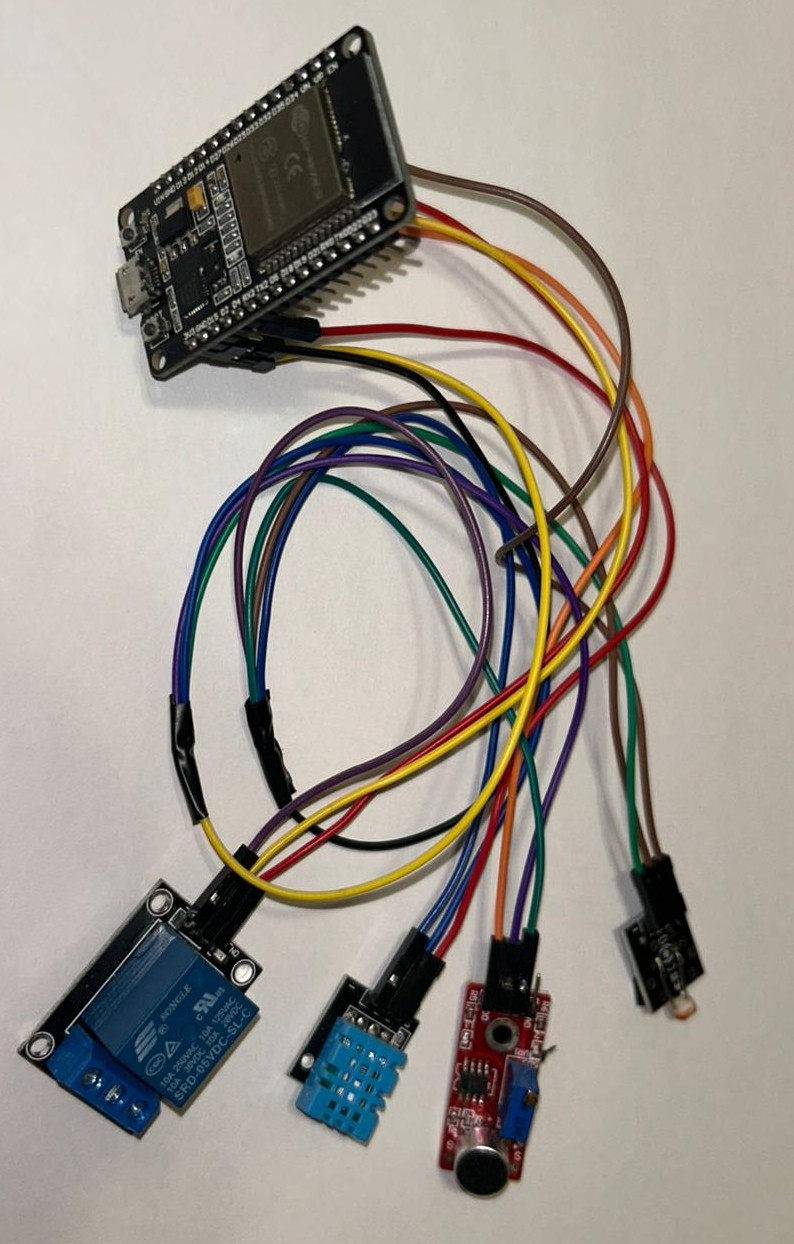
\includegraphics[width=0.7\textwidth]{Img/nodo_ambiente.jpg}
    \caption{Prototipo físico y conexionado de componentes del Nodo 1 (Nodo Ambiente).}
    \label{fig:foto_nodo1}
\end{figure}

\subsubsection{Nodo 2: telemetría espacial y disuasión óptica (nodo escritorio)}
Situado de forma estratégica en el área de trabajo para garantizar la cobertura directa del plano del usuario, este nodo asume las tareas de detección biométrica volumétrica y señalización perimetral mediante la integración de dos subsistemas principales:
\begin{itemize}
    \item \textbf{Transductor volumétrico:} el radar de ondas milimétricas HLK-LD2410C, interconectado con el soc ESP32 a través de un bus de comunicación serie UART (\textit{universal asynchronous receiver-transmitter}) empleando los pines dedicados de transmisión (TX) y recepción (RX). Esta interfaz de alta velocidad permite extraer de manera síncrona los vectores de energía y distancia correspondientes a objetivos dinámicos y estacionarios.
    \item \textbf{Emisor óptico:} un módulo de diodo láser semiconductor conectado a un pin GPIO configurado como salida digital. Este componente actúa como un dispositivo indicador físico de estado y disuasión perimetral, gobernado por el motor algorítmico durante el armado del sistema de alarma o como señal de advertencia secundaria en los ciclos lógicos de trabajo.
\end{itemize}

\begin{figure}[H]
    \centering
    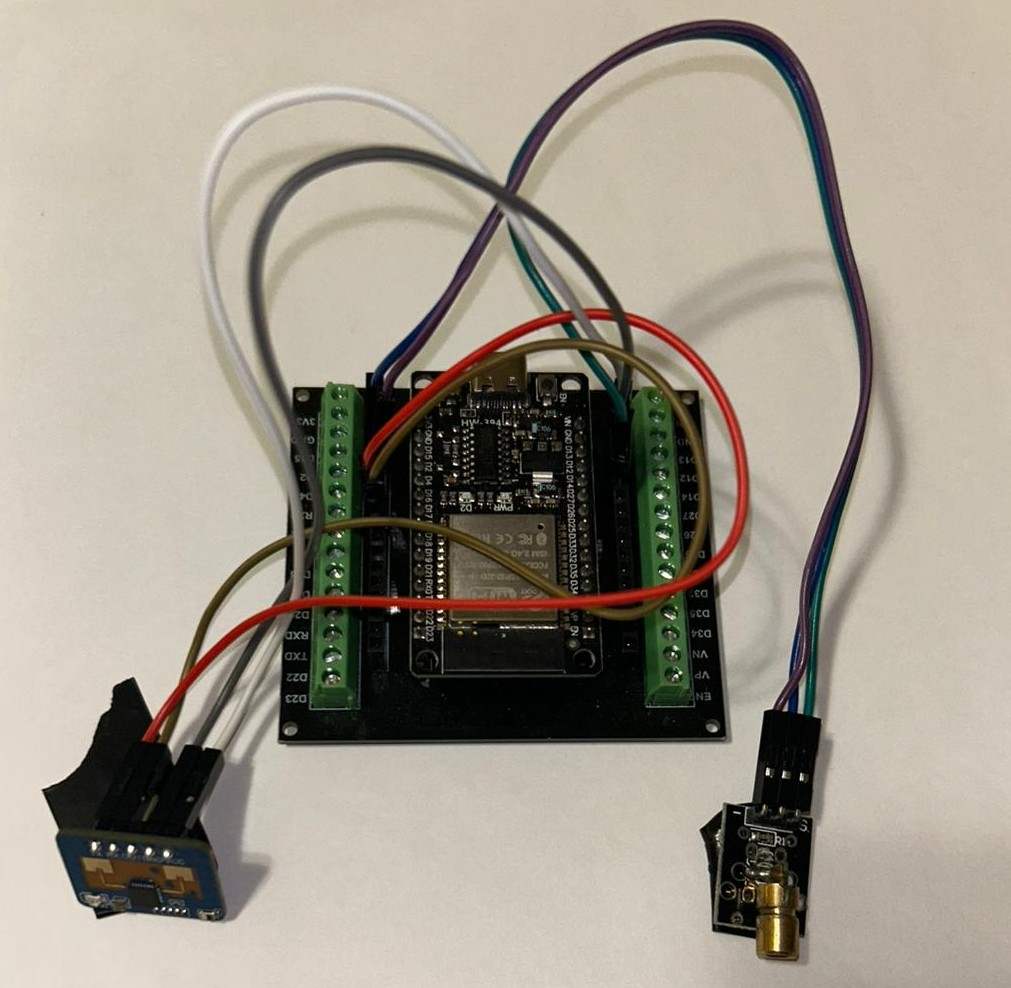
\includegraphics[width=0.7\textwidth]{Img/nodo_escritorio.jpg}
    \caption{Prototipo físico y conexionado de componentes del Nodo 2 (Nodo Escritorio).}
    \label{fig:foto_nodo2}
\end{figure}

\subsubsection{Nodo 3: seguridad perimetral y control de acceso (nodo puerta)}
Ubicado de forma fija en el acceso principal de la estancia, este nodo asume la función exclusiva de supervisar la integridad perimetral del espacio para nutrir el subsistema de alarma. Integra un transductor de contacto magnético de tipo interruptor reed, cuyo funcionamiento se basa en la conmutación eléctrica ante la proximidad de un campo magnético solidario a la hoja de la puerta. El sensor se conecta directamente a un pin GPIO configurado como entrada digital con resistencia de polarización activa (\textit{pull-up}). Las transiciones de estado físico abren o cierran el circuito, disparando interrupciones por hardware en el microcontrolador para garantizar el registro inmediato del evento y mitigar los retardos asociados al muestreo por sondeo (\textit{polling}), transmitiendo la condición de apertura o cierre de forma instantánea hacia el agente de comunicaciones.

\begin{figure}[H]
    \centering
    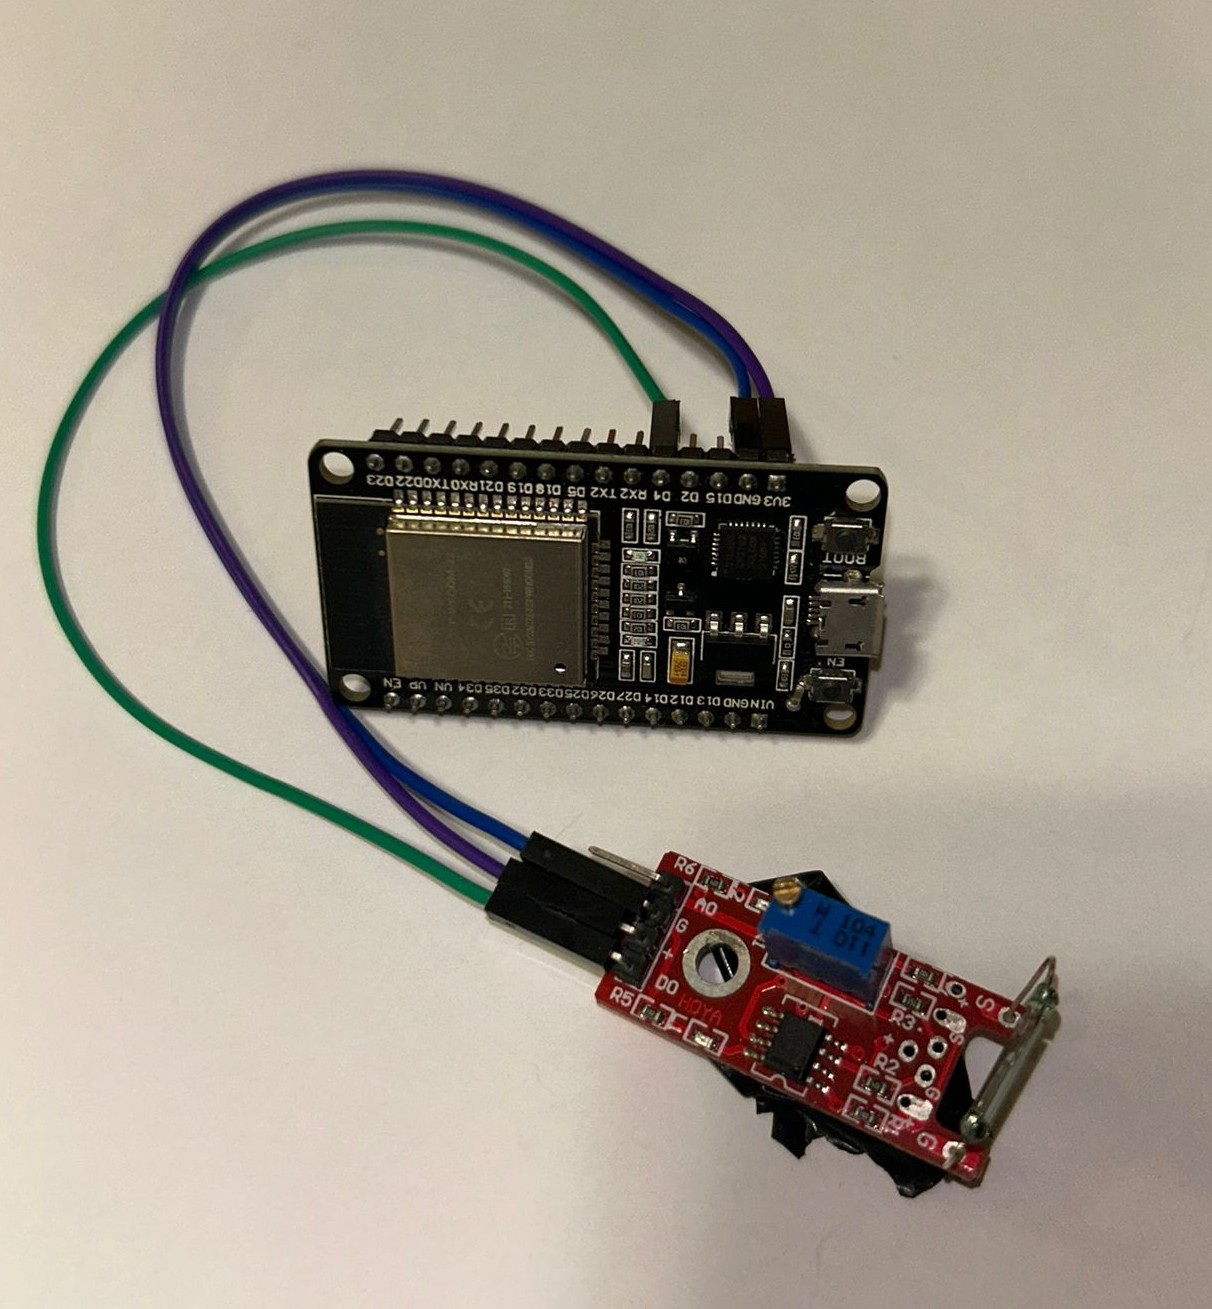
\includegraphics[width=0.7\textwidth]{Img/nodo_puerta.jpg}
    \caption{Prototipo físico e instalación del interruptor magnético del Nodo 3 (Nodo Puerta).}
    \label{fig:foto_nodo3}
\end{figure}

\subsection{Diseño del algoritmo de fusión de sensores (motor de contexto)}
El comportamiento adaptativo del sistema se gobierna mediante una máquina de estados finitos (FSM, por sus siglas en inglés) que ejecuta la fusión de datos en el extremo (\textit{edge}). El sistema abstrae la situación del entorno en cuatro estados discretos estables: \textbf{ausente}, \textbf{ocio}, \textbf{estudio} y \textbf{durmiendo}.

La transición entre estados no depende de un único sensor aislado, sino del procesamiento condicional cruzado de la telemetría entrante, aplicando redundancia lógica para garantizar la tolerancia a fallos. El modelo matemático de transiciones se rige por las siguientes reglas de inferencia:

\begin{equation}
\text{Transición a estudio: } \{ P_{\text{mmWave}} = 1 \} \land \{ D_{\text{objetivo}} \le R_{\text{escritorio}} \} \land \{ T_{\text{estudio}} \ge t_{\text{filtro}} \}
\end{equation}

Donde $P_{\text{mmWave}}$ representa la presencia detectada por el radar, $D_{\text{objetivo}}$ es la distancia cuantitativa registrada y $R_{\text{escritorio}}$ delimita el radio físico del área de trabajo. Un temporizador de seguridad ($t_{\text{filtro}}$) evita falsas transiciones por cruces esporádicos.

Para solventar contingencias críticas de hardware (como la degradación o fallo de lectura de un sensor individual), el algoritmo incorpora bucles de redundancia y reseteo activo. Si el sistema se encuentra en estado \textbf{durmiendo} debido a una lectura baja fija del LDR provocada por un fallo eléctrico, pero el canal analógico del radar computa una ausencia prolongada ($P_{\text{mmWave}} = 0$) durante un tiempo continuo $t_{\text{ausencia}} \ge 20 \text{ minutos}$, el motor de contexto anula de forma proactiva la prioridad del sensor lumínico, forzando la transición segura al estado \textbf{ausente} y mitigando el congelamiento lógico de la infraestructura.

\begin{figure}[H]
    \centering
    \begin{tikzpicture}[
        state/.style={
            circle,
            draw=Azul!80,
            fill=Azul!10,
            very thick,
            minimum size=2.4cm,
            align=center,
            font=\bfseries\small
        },
        trans/.style={
            ->,
            >=stealth,
            thick,
            draw=gray!80,
            align=center,
            font=\scriptsize
        }
    ]
        % Nodes with increased spacing (7.5cm horizontal, 5.0cm vertical)
        \node[state, fill=Rojo!10, draw=Rojo!80] (ausente) at (0, 5.0) {Ausente};
        \node[state, fill=Naranja!10, draw=Naranja!80] (ocio) at (7.5, 5.0) {Ocio};
        \node[state, fill=Verde!10, draw=Verde!80] (estudio) at (7.5, 0.0) {Estudio};
        \node[state, fill=Morado!10, draw=Morado!80] (durmiendo) at (0, 0.0) {Durmiendo};

        % Transitions with clean bend curves and wrapped labels
        \path (ausente) edge[trans, bend left=20] node[above, midway] {Presencia\\($P_{\text{mmWave}} = 1$)} (ocio);
        \path (ocio) edge[trans, bend left=20] node[below, midway] {Ausencia\\($P_{\text{mmWave}} = 0$)} (ausente);
        
        \path (ocio) edge[trans, bend left=20] node[right, midway] {En escritorio y\\$T_{\text{estudio}} \ge t_{\text{filtro}}$} (estudio);
        \path (estudio) edge[trans, bend left=20] node[left, midway] {Fuera de\\escritorio} (ocio);
        
        \path (estudio) edge[trans, bend left=20] node[below, midway] {Luz LDR $\le$ umbral\\y reposo} (durmiendo);
        \path (durmiendo) edge[trans, bend left=20] node[above, midway] {Presencia o\\movimiento} (estudio);
        
        \path (durmiendo) edge[trans, bend left=20] node[left, midway] {Ausencia\\$\ge 20$ min\\(redundancia)} (ausente);
        \path (ausente) edge[trans, bend left=20] node[right, midway] {Modo noche\\y reposo} (durmiendo);
    \end{tikzpicture}
    \caption{Diagrama de la Máquina de Estados Finitos (FSM) para la inferencia de estados contextuales.}
    \label{fig:fsm_estados}
\end{figure}

\subsection{Diseño de la base de datos y flujos de información}
El flujo de información sigue un modelo síncrono y bidireccional basado en la API nativa de ESPHome \cite{al2015internet}. Los nodos sensores operan de forma autónoma, digitalizando las variables térmicas, lumínicas y espaciales a una frecuencia de muestreo parametrizada. Cada lectura actualiza una entidad expuesta en el servidor a través de sockets TCP directos en el puerto 6053, sin necesidad de parsear tramas de texto complejas ni depender de brokers de mensajería intermedios.

El servidor central central captura las actualizaciones de estado de manera inmediata. Al recibir un nuevo evento, se despierta el hilo de ejecución del motor de contexto, que evalúa las condiciones de la FSM. Si se determina un cambio de estado, se genera un evento interno en el bus de Home Assistant que dispara dos acciones concurrentes:
\begin{enumerate}
    \item \textbf{Actuación perimetral:} se invoca el servicio de conmutación correspondiente de vuelta hacia el nodo ESP32 a través del canal abierto de la API, forzando la activación física del relé.
    \item \textbf{Persistencia temporal:} el estado indexado y la telemetría asociada se envían al subsistema de almacenamiento local. La base de datos, estructurada como un motor de series temporales de ejecución en memoria con volcado cíclico al almacenamiento secundario local, registra la tupla compuesta por el identificador de la entidad, el valor transformado y la marca de tiempo precisa (\textit{timestamp}) proporcionada por el sistema operativo del servidor. Esto permite la auditoría posterior de las rutinas del usuario sin comprometer datos fuera de la red local.
\end{enumerate}

\begin{figure}[H]
    \centering
    \begin{tikzpicture}[
        block/.style={
            rectangle,
            draw=Azul!80,
            fill=Azul!10,
            rounded corners=2pt,
            thick,
            minimum width=3.2cm,
            minimum height=1.1cm,
            align=center,
            font=\bfseries\footnotesize
        },
        arrow/.style={
            ->,
            >=stealth,
            thick,
            draw=gray!80
        },
        txt/.style={
            align=center,
            font=\scriptsize\itshape
        }
    ]
        % Nodes
        \node[block, fill=Naranja!10, draw=Naranja!80] (sensores) at (-4.0, 1.5) {Nodos de Control\\(ESP32)};
        \node[block, fill=Azul!10, draw=Azul!80] (ha) at (4.0, 1.5) {Servidor central\\(Home Assistant)};
        \node[block, fill=Morado!10, draw=Morado!80] (db) at (4.0, -1.8) {Persistencia\\(Base de Datos)};
        \node[block, fill=Rojo!10, draw=Rojo!80] (rele) at (-4.0, -1.8) {Actuador\\(Módulo Relé)};

        % Paths
        \draw[arrow] (sensores) to[bend left=20] node[above, txt] {1. Actualiza estado\\(Socket TCP / ProtoBuf)} (ha);
        \draw[arrow] (ha) to[bend left=20] node[below, txt] {2. Ordena conmutación\\(API nativa ESPHome)} (sensores);
        \draw[arrow] (ha) -- node[right, txt] {3. Registra\\series\\temporales} (db);
        \draw[arrow] (sensores) -- node[left, txt] {4. Conmutación\\física (GPIO)} (rele);
    \end{tikzpicture}
    \caption{Diagrama de flujos de información e integración mediante la API nativa de ESPHome en la red local.}
    \label{fig:flujo_informacion}
\end{figure}

\subsection{Análisis de frecuencias y coexistencia (banda ISM)}
Tanto la red troncal Wi-Fi como la red sensórica secundaria operan en la banda ISM de 2.4 GHz. Para evitar interferencias y pérdida de paquetes, se implementa una estrategia de coexistencia de espectro:
\begin{itemize}
    \item \textbf{Capa WLAN:} se configura de forma estática en uno de los tres canales no superpuestos (1, 6 u 11) con un ancho de banda de 20 MHz.
    \item \textbf{Capa WPAN (BLE):} utiliza los canales 37, 38 y 39 en exclusiva para las tramas pasivas (\textit{advertising}) de los sensores. Estos canales se sitúan en los extremos y huecos de la banda, esquivando las frecuencias centrales Wi-Fi. Para las comunicaciones activas, se emplea el algoritmo AFH (\textit{Adaptive Frequency Hopping}) para esquivar el espectro saturado por la WLAN.
\end{itemize}

\subsection{Protocolos de comunicación y modelo OSI}
El flujo de información atraviesa dos pilas de protocolos distintas. Las placas ESP32 actúan como pasarelas de aplicación (\textit{application layer gateways}) para unificar el entorno perimetral:

\begin{table}[H]
    \centering
    \setlength{\tabcolsep}{4pt}
    \renewcommand{\arraystretch}{1.2}
    \begin{tabular}{|c|c|c|}
        \hhline{|-|-|-|}
        \rowcolor[gray]{0.9} 
        \parbox[c]{3.5cm}{\vspace{0.2cm}\centering\textbf{Capa OSI}\vspace{0.2cm}} & \parbox[c]{5.25cm}{\vspace{0.2cm}\centering\textbf{Red sensórica (WPAN)}\vspace{0.2cm}} & \parbox[c]{5.25cm}{\vspace{0.2cm}\centering\textbf{Red troncal (WLAN)}\vspace{0.2cm}} \\ \hhline{|-|-|-|}
        \parbox[c]{3.5cm}{\vspace{0.2cm}\centering\textbf{7. Aplicación}\vspace{0.2cm}} & \parbox[c]{5.25cm}{\vspace{0.2cm}\centering Perfiles GAP / GATT (tramas \textit{advertising})\vspace{0.2cm}} & \parbox[c]{5.25cm}{\vspace{0.2cm}\centering API nativa ESPHome\vspace{0.2cm}} \\ \hhline{|-|-|-|}
        \parbox[c]{3.5cm}{\vspace{0.2cm}\centering\textbf{6. Presentación}\vspace{0.2cm}} & \parbox[c]{5.25cm}{\vspace{0.2cm}\centering Integrado en capa 7\vspace{0.2cm}} & \parbox[c]{5.25cm}{\vspace{0.2cm}\centering Protocol Buffers (binario)\vspace{0.2cm}} \\ \hhline{|-|-|-|}
        \parbox[c]{3.5cm}{\vspace{0.2cm}\centering\textbf{5. Sesión}\vspace{0.2cm}} & \parbox[c]{5.25cm}{\vspace{0.2cm}\centering Sin conexión (\textit{connectionless})\vspace{0.2cm}} & \parbox[c]{5.25cm}{\vspace{0.2cm}\centering Sockets TCP persistentes\vspace{0.2cm}} \\ \hhline{|-|-|-|}
        \parbox[c]{3.5cm}{\vspace{0.2cm}\centering\textbf{4. Transporte}\vspace{0.2cm}} & \parbox[c]{5.25cm}{\vspace{0.2cm}\centering No aplica en topología pasiva\vspace{0.2cm}} & \parbox[c]{5.25cm}{\vspace{0.2cm}\centering TCP (con control de flujo)\vspace{0.2cm}} \\ \hhline{|-|-|-|}
        \parbox[c]{3.5cm}{\vspace{0.2cm}\centering\textbf{3. Red}\vspace{0.2cm}} & \parbox[c]{5.25cm}{\vspace{0.2cm}\centering No aplica en topología punto a punto\vspace{0.2cm}} & \parbox[c]{5.25cm}{\vspace{0.2cm}\centering IPv4 (Enrutamiento local)\vspace{0.2cm}} \\ \hhline{|-|-|-|}
        \parbox[c]{3.5cm}{\vspace{0.2cm}\centering\textbf{1 y 2. Física / Enlace}\vspace{0.2cm}} & \parbox[c]{5.25cm}{\vspace{0.2cm}\centering Direccionamiento MAC BLE. Modulación GFSK (banda 2.4 GHz).\vspace{0.2cm}} & \parbox[c]{5.25cm}{\vspace{0.2cm}\centering Direccionamiento MAC Wi-Fi. IEEE 802.11ax (OFDMA).\vspace{0.2cm}} \\ \hhline{|-|-|-|}
    \end{tabular}
    \caption{Pila de protocolos y mapeo del Modelo OSI en la arquitectura de red.}
    \label{tab:protocolos_osi}
\end{table}

\textbf{Mecanismo de consistencia y control de flujo:}
Al operar sobre la API nativa de ESPHome, se prescinde de la capa de sobrecarga de QoS de MQTT. En su lugar, el protocolo de ESPHome emplea sockets TCP persistentes orientados a conexión que garantizan la entrega en orden de todas las tramas de datos. La API implementa un mecanismo de latido activo (\textit{keepalive}) para detectar desconexiones en un plazo inferior a 5 segundos, y un sistema de cola en memoria local para registrar eventos transitorios y retransmitirlos automáticamente al restablecer el enlace con el servidor central.
\newpage
\section{Selección de tecnologías e integración}
\label{cap:seleccion_tecnologias}

Una vez definida la arquitectura conceptual y funcional del sistema, es necesario concretar y justificar la selección de los componentes físicos y lógicos que materializan la infraestructura. En este capítulo se exponen los criterios técnicos que guiaron la elección de los dispositivos de hardware, los sensores y actuadores específicos utilizados en los tres nodos, así como las plataformas de software y protocolos elegidos para garantizar la interoperabilidad local, la privacidad y la resiliencia del entorno.

\subsection{Criterios de selección}
La ingeniería de diseño para entornos residenciales de inteligencia ambiental exige el cumplimiento de tres restricciones primarias: viabilidad económica, eficiencia energética para operaciones ininterrumpidas (24/7) y madurez tecnológica que asegure la estabilidad de los controladores. Para este proyecto, se priorizó la adopción de hardware comercial de bajo coste y plataformas de software de código abierto. Este enfoque mitiga la dependencia de licencias propietarias y permite un acceso de bajo nivel a los registros de compilación y firmware, propiedad indispensable para implementar algoritmos personalizados de fusión sensorial y control perimetral.

\subsection{Selección de hardware}

\subsubsection{Unidad central de procesamiento (servidor local)}
Para el núcleo computacional y de persistencia de datos se seleccionó el microordenador \textbf{Raspberry Pi 4 Model B} en su variante de 1 GB de memoria RAM LPDDR4. Frente a opciones de menor cómputo como su predecesora (Raspberry Pi 3B+) o alternativas de mayor coste y consumo (arquitecturas x86 tradicionales), la Raspberry Pi 4 ofrece un equilibrio óptimo al integrar un procesador ARM Cortex-A72 de cuatro núcleos a 1.5 GHz. Esta capacidad de procesamiento en paralelo es suficiente para ejecutar simultáneamente el entorno de contenedores Docker, la base de datos local y el motor de automatizaciones lógicas, manteniendo un consumo nominal inferior a los 15 vatios bajo carga máxima, lo que facilita el respaldo del sistema ante contingencias eléctricas mediante Sistemas de Alimentación Ininterrumpida (SAI) de baja potencia.

\begin{table}[H]
    \centering
    \setlength{\tabcolsep}{3pt}
    \renewcommand{\arraystretch}{1.2}
    \begin{tabular}{|c|c|c|c|}
        \hline
        \rowcolor[gray]{0.9} 
        \parbox[c]{4.6cm}{\vspace{0.2cm}\centering\textbf{Características}\vspace{0.2cm}} & \parbox[c]{2.9cm}{\vspace{0.2cm}\centering\textbf{Raspberry Pi 4B}\vspace{0.2cm}} & \parbox[c]{2.9cm}{\vspace{0.2cm}\centering\textbf{Raspberry Pi 3B+}\vspace{0.2cm}} & \parbox[c]{2.9cm}{\vspace{0.2cm}\centering\textbf{Orange Pi 5 Plus}\vspace{0.2cm}} \\ \hline
        \parbox[c]{4.6cm}{\vspace{0.2cm}\centering\textbf{Procesador (CPU)}\vspace{0.2cm}} & \parbox[c]{2.9cm}{\vspace{0.2cm}\centering Cortex-A72 (4x @ 1.5GHz)\vspace{0.2cm}} & \parbox[c]{2.9cm}{\vspace{0.2cm}\centering Cortex-A53 (4x @ 1.4GHz)\vspace{0.2cm}} & \parbox[c]{2.9cm}{\vspace{0.2cm}\centering RK3588 (Octa Core)\vspace{0.2cm}} \\ \hline
        \parbox[c]{4.6cm}{\vspace{0.2cm}\centering\textbf{Memoria RAM}\vspace{0.2cm}} & \parbox[c]{2.9cm}{\vspace{0.2cm}\centering 1GB (LPDDR4)\vspace{0.2cm}} & \parbox[c]{2.9cm}{\vspace{0.2cm}\centering 1GB (LPDDR2)\vspace{0.2cm}} & \parbox[c]{2.9cm}{\vspace{0.2cm}\centering 8GB/\allowbreak 16GB\vspace{0.2cm}} \\ \hline
        \parbox[c]{4.6cm}{\vspace{0.2cm}\centering\textbf{Almacenamiento}\vspace{0.2cm}} & \parbox[c]{2.9cm}{\vspace{0.2cm}\centering MicroSD / USB 3.0\vspace{0.2cm}} & \parbox[c]{2.9cm}{\vspace{0.2cm}\centering MicroSD / USB 2.0\vspace{0.2cm}} & \parbox[c]{2.9cm}{\vspace{0.2cm}\centering Ranura M.2 NVMe\vspace{0.2cm}} \\ \hline
        \parbox[c]{4.6cm}{\vspace{0.2cm}\centering\textbf{Consumo}\vspace{0.2cm}} & \parbox[c]{2.9cm}{\vspace{0.2cm}\centering 3W / 6W\vspace{0.2cm}} & \parbox[c]{2.9cm}{\vspace{0.2cm}\centering 2.5W / 5W\vspace{0.2cm}} & \parbox[c]{2.9cm}{\vspace{0.2cm}\centering 5W / 12W+\vspace{0.2cm}} \\ \hline
        \parbox[c]{4.6cm}{\vspace{0.2cm}\centering\textbf{Inteligencia artificial}\vspace{0.2cm}} & \parbox[c]{2.9cm}{\vspace{0.2cm}\centering Procesamiento CPU\vspace{0.2cm}} & \parbox[c]{2.9cm}{\vspace{0.2cm}\centering Inviable\vspace{0.2cm}} & \parbox[c]{2.9cm}{\vspace{0.2cm}\centering NPU (6 TOPS)\vspace{0.2cm}} \\ \hline
        \parbox[c]{4.6cm}{\vspace{0.2cm}\centering\textbf{Soporte software}\vspace{0.2cm}} & \parbox[c]{2.9cm}{\vspace{0.2cm}\centering Excelente\vspace{0.2cm}} & \parbox[c]{2.9cm}{\vspace{0.2cm}\centering Excelente\vspace{0.2cm}} & \parbox[c]{2.9cm}{\vspace{0.2cm}\centering Limitado/\allowbreak Fragmentado\vspace{0.2cm}} \\ \hline
        \parbox[c]{4.6cm}{\vspace{0.2cm}\centering\textbf{Coste aprox.}\vspace{0.2cm}} & \parbox[c]{2.9cm}{\vspace{0.2cm}\centering Medio (45-55€)\vspace{0.2cm}} & \parbox[c]{2.9cm}{\vspace{0.2cm}\centering Bajo (35€)\vspace{0.2cm}} & \parbox[c]{2.9cm}{\vspace{0.2cm}\centering Alto (140-160€)\vspace{0.2cm}} \\ \hline
    \end{tabular}
    \caption{Comparativa de hardware para el nodo central.}
    \label{tab:hw_central}
\end{table}

A pesar de la superioridad en especificaciones puras de la Orange Pi 5 Plus (recogida en la Tabla~\ref{tab:hw_central}), la Raspberry Pi 4B resulta óptima debido a su eficiencia energética (vital para maximizar la autonomía del SAI ante cortes eléctricos) y la estabilidad de su ecosistema de software. Su arquitectura y cantidad de memoria RAM física (1 GB) son suficientes para ejecutar con solvencia los servicios del motor de inferencia y la base de datos en tiempo real, garantizando una alta estabilidad sin necesidad de sobredimensionar los recursos de la infraestructura (\textit{overprovisioning}).

\subsubsection{Microcontroladores de red (nodos de instrumentación)}
Como elementos de control embebido distribuido se seleccionaron placas de desarrollo basadas en el SoC \textbf{ESP32} de Espressif Systems. Los factores técnicos que justifican esta decisión frente a arquitecturas alternativas (como las plataformas Arduino tradicionales o los microcontroladores PIC) son:
\begin{itemize}
    \item Integración nativa en chip de conectividad inalámbrica Wi-Fi 802.11 b/g/n y Bluetooth v4.2 BR/EDR y BLE.
    \item CPU de doble núcleo Xtensa de 32 bits operando a 240 MHz con 520 KB de SRAM interna, permitiendo la gestión síncrona de interrupciones por hardware de sensores críticos y la serialización asíncrona de tramas de red.
    \item Amplia disponibilidad de canales de conversión analógico-digital (ADC) con resolución parametrizable y transceptores UART por hardware independientes.
\end{itemize}

\subsubsection{Sensores y actuadores de la infraestructura física}
De acuerdo con la distribución empírica diseñada para cubrir las necesidades analíticas y de seguridad del espacio, los transductores específicos seleccionados son:
\begin{itemize}
    \item \textbf{Radar de ondas milimétricas HLK-LD2410C:} dispositivo FMCW operando en la banda de 24 GHz. Se seleccionó por su capacidad analítica para segmentar la energía reflejada en compuertas de distancia fijas y discriminar micromovimientos asociados a la respiración humana, superando la limitación volumétrica de los sensores piroeléctricos.
    \item \textbf{Módulo de sonido de alta sensibilidad (Big Sound):} equipado con un micrófono de electret y el circuito comparador analógico LM393. Permite establecer un umbral de conmutación digital rápido mediante potenciómetro y capturar la amplitud de la señal analógica para auditorías de ruido ambiental.
    \item \textbf{Transductor termo-higrométrico digital:} sensor climático que proporciona lecturas directas calibradas en origen de temperatura exterior y humedad relativa mediante un protocolo serie propietario de un solo hilo, reduciendo el uso de pines GPIO en el Nodo Ambiente.
    \item \textbf{Fotorresistor LDR:} sensor de sulfuro de cadmio (CdS) integrado en un divisor de tensión pasivo. Proporciona una respuesta analógica inversamente proporcional a la iluminancia incidente, idónea para la calibración del comportamiento lumínico de la estancia.
    \item \textbf{Módulo de relé optoacoplado:} actuador de potencia con aislamiento galvánico provisto por un optoacoplador interno. Su inclusión previene el retorno de corrientes parásitas de alta tensión o transitorios de conmutación de la luminaria de corriente alterna hacia las líneas lógicas de baja tensión del ESP32.
    \item \textbf{Módulo de diodo láser semiconductor:} emisor de luz monocromática focalizada de baja potencia. Actúa como transductor de señalización óptica y disuasión perimetral dentro de las reglas de control de la estancia.
    \item \textbf{Sensor magnético de contacto Reed:} interruptor encapsulado que se activa por campo magnético. Instalado en el perfil estructural del acceso principal para el envío de señales binarias inmediatas ante cambios de geometría en la puerta.
\end{itemize}

\begin{table}[H]
    \centering
    \setlength{\tabcolsep}{4pt}
    \renewcommand{\arraystretch}{1.2}
    \begin{tabular}{|c|c|c|}
        \hline
        \rowcolor[gray]{0.9} 
        \parbox[c]{3.2cm}{\vspace{0.2cm}\centering\textbf{Métrica}\vspace{0.2cm}} & \parbox[c]{5.2cm}{\vspace{0.2cm}\centering\textbf{Sensor infrarrojo (PIR)}\vspace{0.2cm}} & \parbox[c]{5.2cm}{\vspace{0.2cm}\centering\textbf{Radar mmWave (HLK-LD2410C)}\vspace{0.2cm}} \\ \hline
        \parbox[c]{3.2cm}{\vspace{0.2cm}\centering\textbf{Principio}\vspace{0.2cm}} & \parbox[c]{5.2cm}{\vspace{0.2cm}\centering Radiación térmica (infrarrojo)\vspace{0.2cm}} & \parbox[c]{5.2cm}{\vspace{0.2cm}\centering Radiofrecuencia modulada (FMCW 24 GHz)\vspace{0.2cm}} \\ \hline
        \parbox[c]{3.2cm}{\vspace{0.2cm}\centering\textbf{Detección estática}\vspace{0.2cm}} & \parbox[c]{5.2cm}{\vspace{0.2cm}\centering Nula (falsos negativos frecuentes)\vspace{0.2cm}} & \parbox[c]{5.2cm}{\vspace{0.2cm}\centering Alta (detecta micromovimientos y respiración)\vspace{0.2cm}} \\ \hline
        \parbox[c]{3.2cm}{\vspace{0.2cm}\centering\textbf{Precisión espacial}\vspace{0.2cm}} & \parbox[c]{5.2cm}{\vspace{0.2cm}\centering Binaria (presencia/ausencia)\vspace{0.2cm}} & \parbox[c]{5.2cm}{\vspace{0.2cm}\centering Cuantitativa (distancia en cm)\vspace{0.2cm}} \\ \hline
        \parbox[c]{3.2cm}{\vspace{0.2cm}\centering\textbf{Sensibilidad ambiental}\vspace{0.2cm}} & \parbox[c]{5.2cm}{\vspace{0.2cm}\centering Propenso a falsos positivos (sol, calor)\vspace{0.2cm}} & \parbox[c]{5.2cm}{\vspace{0.2cm}\centering Inmune a cambios térmicos\vspace{0.2cm}} \\ \hline
        \parbox[c]{3.2cm}{\vspace{0.2cm}\centering\textbf{Ocultación}\vspace{0.2cm}} & \parbox[c]{5.2cm}{\vspace{0.2cm}\centering Requiere línea de visión directa\vspace{0.2cm}} & \parbox[c]{5.2cm}{\vspace{0.2cm}\centering Alta penetración (atraviesa plásticos)\vspace{0.2cm}} \\ \hline
    \end{tabular}
    \caption{Comparativa técnica entre sensores PIR y radares FMCW.}
    \label{tab:pir_vs_mmwave_comp}
\end{table}

Tal y como se detalla en la comparativa técnica de la Tabla~\ref{tab:pir_vs_mmwave_comp}, la tecnología FMCW aprovecha el efecto Doppler a alta frecuencia para discriminar pequeñas variaciones de la caja torácica humana durante la respiración, eliminando los falsos negativos que sufren los sensores PIR convencionales cuando un usuario se encuentra inmóvil.

\subsection{Selección de software y protocolos}

\subsubsection{Firmware declarativo del hardware embebido}
Para la programación e instrumentación de los microcontroladores se descartó el desarrollo de código monolítico imperativo en entornos tradicionales en favor de \textbf{ESPHome}. Esta herramienta permite generar firmwares optimizados a partir de archivos de configuración declarativos estructurados en formato YAML. ESPHome compila directamente sobre el framework original del fabricante, abstrayendo la gestión del stack TCP/IP y garantizando la reconexión automática ante pérdidas de señal inalámbrica. El uso de este sistema facilita la monitorización de registros en tiempo real (\textit{logs}) directamente desde el orquestador central y permite actualizaciones inalámbricas seguras (OTA, por sus siglas en inglés).

\subsubsection{Orquestador central y motor de contexto}
El núcleo lógico del sistema se sustenta sobre \textbf{Home Assistant Container} ejecutado en un entorno aislado de contenedores. Se seleccionó esta plataforma de código abierto debido a su arquitectura dirigida por eventos y su capacidad para unificar sistemas heterogéneos bajo una capa común de entidades lógicas. Home Assistant asume el rol de Motor de Contexto, ejecutando las automatizaciones locales complejas, gestionando las máquinas de estado finito de la estancia y aislando por completo la lógica operacional de servidores de terceros en la nube, siguiendo patrones de diseño específicos para la orquestación confiable en el borde \cite{pahl2018trusted}.

\begin{table}[H]
    \centering
    \setlength{\tabcolsep}{3pt}
    \renewcommand{\arraystretch}{1.2}
    \begin{tabular}{|c|c|c|c|c|}
        \hline
        \rowcolor[gray]{0.9} 
        \parbox[c]{4.5cm}{\vspace{0.2cm}\centering\textbf{Características}\vspace{0.2cm}} & \parbox[c]{2.4cm}{\vspace{0.2cm}\centering\textbf{Home Assistant}\vspace{0.2cm}} & \parbox[c]{2.2cm}{\vspace{0.2cm}\centering\textbf{OpenHAB}\vspace{0.2cm}} & \parbox[c]{2.1cm}{\vspace{0.2cm}\centering\textbf{Domoticz}\vspace{0.2cm}} & \parbox[c]{2.5cm}{\vspace{0.2cm}\centering\textbf{Ecosistemas comerciales}\vspace{0.2cm}} \\ \hline
        \parbox[c]{4.5cm}{\vspace{0.2cm}\centering\textbf{Arquitectura}\vspace{0.2cm}} & \parbox[c]{2.4cm}{\vspace{0.2cm}\centering Dirigido por eventos (Python)\vspace{0.2cm}} & \parbox[c]{2.2cm}{\vspace{0.2cm}\centering Java (pesado)\vspace{0.2cm}} & \parbox[c]{2.1cm}{\vspace{0.2cm}\centering C++ (ligero)\vspace{0.2cm}} & \parbox[c]{2.5cm}{\vspace{0.2cm}\centering Basado en la nube\vspace{0.2cm}} \\ \hline
        \parbox[c]{4.5cm}{\vspace{0.2cm}\centering\textbf{Primero local}\vspace{0.2cm}} & \parbox[c]{2.4cm}{\vspace{0.2cm}\centering Nativo (sin internet)\vspace{0.2cm}} & \parbox[c]{2.2cm}{\vspace{0.2cm}\centering Nativo\vspace{0.2cm}} & \parbox[c]{2.1cm}{\vspace{0.2cm}\centering Nativo\vspace{0.2cm}} & \parbox[c]{2.5cm}{\vspace{0.2cm}\centering No\vspace{0.2cm}} \\ \hline
        \parbox[c]{4.5cm}{\vspace{0.2cm}\centering\textbf{Integraciones}\vspace{0.2cm}} & \parbox[c]{2.4cm}{\vspace{0.2cm}\centering +2500\vspace{0.2cm}} & \parbox[c]{2.2cm}{\vspace{0.2cm}\centering +/- 400\vspace{0.2cm}} & \parbox[c]{2.1cm}{\vspace{0.2cm}\centering +/- 300\vspace{0.2cm}} & \parbox[c]{2.5cm}{\vspace{0.2cm}\centering Limitadas\vspace{0.2cm}} \\ \hline
        \parbox[c]{4.5cm}{\vspace{0.2cm}\centering\textbf{Automatización}\vspace{0.2cm}} & \parbox[c]{2.4cm}{\vspace{0.2cm}\centering UI avanzada + YAML\vspace{0.2cm}} & \parbox[c]{2.2cm}{\vspace{0.2cm}\centering Scripts complejos\vspace{0.2cm}} & \parbox[c]{2.1cm}{\vspace{0.2cm}\centering LUA/\allowbreak Blockly\vspace{0.2cm}} & \parbox[c]{2.5cm}{\vspace{0.2cm}\centering Rutinas básicas\vspace{0.2cm}} \\ \hline
        \parbox[c]{4.5cm}{\vspace{0.2cm}\centering\textbf{Interfaz API}\vspace{0.2cm}} & \parbox[c]{2.4cm}{\vspace{0.2cm}\centering WebSocket (tiempo real)\vspace{0.2cm}} & \parbox[c]{2.2cm}{\vspace{0.2cm}\centering REST API\vspace{0.2cm}} & \parbox[c]{2.1cm}{\vspace{0.2cm}\centering JSON/\allowbreak MQTT\vspace{0.2cm}} & \parbox[c]{2.5cm}{\vspace{0.2cm}\centering REST API\vspace{0.2cm}} \\ \hline
    \end{tabular}
    \caption{Comparativa de ecosistemas de orquestación domótica.}
    \label{tab:sw_domotica}
\end{table}

Frente a los ecosistemas propietarios y soluciones comerciales recogidas en la Tabla~\ref{tab:sw_domotica}, Home Assistant garantiza un procesamiento \textit{edge} 100\% local sin depender de servidores externos, mitigando latencias y protegiendo la privacidad. Frente a OpenHAB, la arquitectura basada en Python de Home Assistant permite compartir el mismo entorno de ejecución con los scripts analíticos de este proyecto (facilitando el uso de NumPy y Pandas), evitando la pesada sobrecarga de la máquina virtual de Java (JVM) en un hardware de recursos restringidos como la Raspberry Pi.

\subsubsection{Estrategia de despliegue}
Home Assistant ofrece cuatro métodos oficiales de instalación. Se debe elegir el método que brinde mayor control y menor impacto sobre el rendimiento del servidor central.

\begin{table}[H]
    \centering
    \setlength{\tabcolsep}{3pt}
    \renewcommand{\arraystretch}{1.2}
    \begin{tabular}{|c|c|c|c|c|}
        \hline
        \rowcolor[gray]{0.9} 
        \parbox[c]{4.5cm}{\vspace{0.2cm}\centering\textbf{Características}\vspace{0.2cm}} & \parbox[c]{2.4cm}{\vspace{0.2cm}\centering\textbf{HA Container (Docker)}\vspace{0.2cm}} & \parbox[c]{1.9cm}{\vspace{0.2cm}\centering\textbf{HA OS}\vspace{0.2cm}} & \parbox[c]{2.4cm}{\vspace{0.2cm}\centering\textbf{HA Core (venv)}\vspace{0.2cm}} & \parbox[c]{2.2cm}{\vspace{0.2cm}\centering\textbf{HA Supervised}\vspace{0.2cm}} \\ \hline
        \parbox[c]{4.5cm}{\vspace{0.2cm}\centering\textbf{Acceso al SO}\vspace{0.2cm}} & \parbox[c]{2.4cm}{\vspace{0.2cm}\centering Total (Raspberry OS)\vspace{0.2cm}} & \parbox[c]{1.9cm}{\vspace{0.2cm}\centering Nulo (cerrado)\vspace{0.2cm}} & \parbox[c]{2.4cm}{\vspace{0.2cm}\centering Total\vspace{0.2cm}} & \parbox[c]{2.2cm}{\vspace{0.2cm}\centering Total\vspace{0.2cm}} \\ \hline
        \parbox[c]{4.5cm}{\vspace{0.2cm}\centering\textbf{Gestión de dependencias}\vspace{0.2cm}} & \parbox[c]{2.4cm}{\vspace{0.2cm}\centering Aislada (contenedor)\vspace{0.2cm}} & \parbox[c]{1.9cm}{\vspace{0.2cm}\centering SO\vspace{0.2cm}} & \parbox[c]{2.4cm}{\vspace{0.2cm}\centering Manual\vspace{0.2cm}} & \parbox[c]{2.2cm}{\vspace{0.2cm}\centering Supervisor\vspace{0.2cm}} \\ \hline
        \parbox[c]{4.5cm}{\vspace{0.2cm}\centering\textbf{Tienda de complementos}\vspace{0.2cm}} & \parbox[c]{2.4cm}{\vspace{0.2cm}\centering No (contenedores)\vspace{0.2cm}} & \parbox[c]{1.9cm}{\vspace{0.2cm}\centering Sí (1 clic)\vspace{0.2cm}} & \parbox[c]{2.4cm}{\vspace{0.2cm}\centering No\vspace{0.2cm}} & \parbox[c]{2.2cm}{\vspace{0.2cm}\centering Sí\vspace{0.2cm}} \\ \hline
        \parbox[c]{4.5cm}{\vspace{0.2cm}\centering\textbf{Flexibilidad}\vspace{0.2cm}} & \parbox[c]{2.4cm}{\vspace{0.2cm}\centering Máxima (microservicios)\vspace{0.2cm}} & \parbox[c]{1.9cm}{\vspace{0.2cm}\centering Baja\vspace{0.2cm}} & \parbox[c]{2.4cm}{\vspace{0.2cm}\centering Alta\vspace{0.2cm}} & \parbox[c]{2.2cm}{\vspace{0.2cm}\centering Media\vspace{0.2cm}} \\ \hline
    \end{tabular}
    \caption{Comparativa de los métodos de instalación de Home Assistant.}
    \label{tab:ha_instalacion}
\end{table}

De acuerdo con el análisis de la Tabla~\ref{tab:ha_instalacion}, se ha seleccionado el despliegue mediante \textbf{Home Assistant Container (Docker)} sobre Raspberry Pi OS Lite. Esta decisión técnica se fundamenta en:
\begin{enumerate}
    \item \textbf{Acceso a nivel de sistema operativo:} vital para la ejecución de scripts en Python personalizados fuera de las restricciones impuestas por el sistema operativo cerrado de HA OS.
    \item \textbf{Arquitectura de microservicios:} mediante \textit{Docker Compose}, se aíslan y gestionan de forma independiente los servicios críticos (el núcleo de Home Assistant Container, el entorno de desarrollo y compilación ESPHome, y el panel de control Portainer), lo que permite que las tareas de administración no afecten a la automatización del hogar.
    \item \textbf{Eficiencia:} al prescindir de la sobrecarga del supervisor integrado en la alternativa *Supervised* o en HA OS, se reduce drásticamente la huella de memoria RAM, liberando recursos para la base de datos y la algoritmia del sistema.
\end{enumerate}

\begin{figure}[H]
    \centering
    \begin{tikzpicture}[
        node/.style={
            rectangle,
            draw=gray!80,
            fill=gray!5,
            rounded corners=5pt,
            thick,
            minimum width=12.0cm,
            minimum height=4.8cm,
            align=left,
            font=\bfseries\small
        },
        container/.style={
            rectangle,
            draw=Azul!80,
            fill=Azul!10,
            rounded corners=2pt,
            thick,
            minimum width=2.6cm,
            minimum height=1.4cm,
            align=center,
            font=\bfseries\scriptsize
        },
        net/.style={
            draw=Verde!80,
            dashed,
            very thick
        }
    ]
        % Main Node (Raspberry Pi 4)
        \node[node] (rpi) at (0, 0) {};
        \node[anchor=north west, font=\bfseries\small, text=gray!80] at ([xshift=0.3cm, yshift=-0.3cm]rpi.north west) {Servidor Central: Raspberry Pi 4 (Raspberry Pi OS Lite)};
        \node[anchor=north west, font=\bfseries\scriptsize\itshape, text=Azul!80] at ([xshift=0.3cm, yshift=-0.7cm]rpi.north west) {Motor de Contenedores Docker};

        % Containers (Portainer, ESPHome, Home Assistant)
        \node[container, fill=Cyan!15, draw=Cyan!80] (portainer) at (-3.6, -0.2) {Portainer\\(Gestión)\\{\normalfont\tiny Puerto: 9000}};
        \node[container, fill=Verde!15, draw=Verde!80] (esphome) at (0, -0.2) {ESPHome\\(Firmware)\\{\normalfont\tiny Puerto: 6052}};
        \node[container, fill=Azul!15, draw=Azul!80] (ha) at (3.6, -0.2) {Home Assistant\\(Núcleo)\\{\normalfont\tiny Puerto: 8123}};

        % Virtual network line
        \draw[net] (-4.9, -1.8) -- (4.9, -1.8) node[above, midway, font=\bfseries\tiny, text=Verde!80] {Docker Bridge Network (172.18.0.0/16)};
        
        % Connections
        \draw[thick, draw=gray!60] (portainer.south) -- (-3.6, -1.8);
        \draw[thick, draw=gray!60] (esphome.south) -- (0, -1.8);
        \draw[thick, draw=gray!60] (ha.south) -- (3.6, -1.8);
        
    \end{tikzpicture}
    \caption{Arquitectura de despliegue basada en microservicios mediante Docker Container en el servidor central.}
    \label{fig:despliegue_docker}
\end{figure}

\subsubsection{Protocolo de comunicaciones}
Para el intercambio de telemetría y eventos de control entre los nodos instrumentados y el servidor central se seleccionó la \textbf{API nativa de ESPHome} sobre conexiones TCP directas en el puerto 6053. A diferencia de protocolos tradicionales basados en texto o intermediarios de mensajería (como HTTP o MQTT), esta API emplea un canal de sockets binarios optimizado mediante estructuras de serialización ligeras (basadas en Google Protocol Buffers). Adicionalmente, el canal incorpora cifrado local mediante el protocolo Noise, garantizando la privacidad del tráfico de sensores. Esta elección tecnológica asegura tiempos de transmisión de eventos inferiores a los 10 milisegundos y proporciona un mecanismo de comprobación activa del estado del enlace (\textit{keepalive}), capacitando al orquestador central para diagnosticar interrupciones de red de manera determinista y tolerar fallos en el bus local \cite{al2015internet}.

\subsection{Integración entre sistemas heterogéneos}
La cohesión de la arquitectura se logra mediante la estandarización de las interfaces de intercambio de datos. Los nodos ESP32 digitalizan los transductores analógicos e interactúan de forma nativa con los sensores digitales empleando buses serie locales (UART, unifilar). Posteriormente, ESPHome traduce esta telemetría física en variables de estado que son expuestas y actualizadas síncronamente hacia el servidor a través del socket binario de la API.

Esta comunicación directa prescinde de brokers de mensajería intermedios (como Eclipse Mosquitto), reduciendo sustancialmente la sobrecarga computacional de la Raspberry Pi 4 de 1 GB. Home Assistant absorbe de forma concurrente los eventos de la API y los mapea inmediatamente a su bus lógico interno de entidades. Esta cadena de integración elimina la necesidad de configurar manualmente tópicos o parsear tramas de datos complejas en el servidor central, permitiendo que el motor de inferencia evalúe de manera uniforme variables físicas tan diversas como la distancia del radar, la caída de tensión del LDR o el estado del interruptor magnético de la puerta, consolidando una infraestructura de computación sensible al contexto robusta, segura y completamente independiente de conectividad externa.

\newpage
\section{Plan de Implantación y Pruebas}
\label{cap:plan_implantacion}

\lstdefinelanguage{YAML}{
  keywords={true,false,null,y,n},
  keywordstyle=\color{blue}\bfseries,
  basicstyle=\ttfamily\footnotesize,
  rulecolor=\color{black},
  aboveskip={1.5\baselineskip},
  columns=fixed,
  showstringspaces=false,
  extendedchars=true,
  breaklines=true,
  backgroundcolor=\color{gray!5},
  frame=single,
  identifierstyle=\color{black},
  stringstyle=\color{orange}\ttfamily,
  commentstyle=\color{teal}\ttfamily,
  sensitive=false,
  comment=[l]{\#},
  morestring=[b]',
  morestring=[b]"
}

La materialización de la arquitectura teórica propuesta exige una metodología rigurosa para el ensamblaje físico, la configuración del \textit{software} perimetral y la validación empírica de todos los subsistemas. En este capítulo se detallan las fases de despliegue del prototipo, el esquema de conexionado físico y de pines de los nodos de instrumentación, y el protocolo de pruebas diseñado para certificar el cumplimiento de los requisitos funcionales, así como la tolerancia a fallos del motor lógico local.

\subsection{Fases del despliegue del sistema}
\label{sec:despliegue}
La implantación de la infraestructura domótica local se ejecutó siguiendo un modelo iterativo e incremental, estructurado en las siguientes fases secuenciales:
\begin{enumerate}
    \item \textbf{Aprovisionamiento y validación analógica:} ensamblaje preliminar de los componentes electrónicos en placa de pruebas (\textit{breadboard}) para la medición de caídas de tensión mediante multímetro, la calibración física de umbrales mediante el potenciómetro de precisión integrado en el módulo de detección acústica y la verificación general del comportamiento eléctrico en frío, minimizando el riesgo de cortocircuitos.
    \item \textbf{Despliegue del núcleo lógico perimetral:} instalación del sistema operativo subyacente (Raspberry Pi OS) en el servidor perimetral (Raspberry Pi 4 con 1\,GB de RAM) y el despliegue del servidor central Home Assistant Container y la suite ESPHome como contenedores independientes aislados en Docker. En esta fase se configuró el motor de base de datos local SQLite y su base de datos (\texttt{home-assistant\_v2.db}), definiendo las políticas de depuración y retención del historial para garantizar el rendimiento en un hardware con limitaciones de memoria y almacenamiento. El estado operativo de los contenedores desplegados se muestra en la Figura~\ref{fig:portainer_containers}.
    
    \begin{figure}[H]
        \centering
        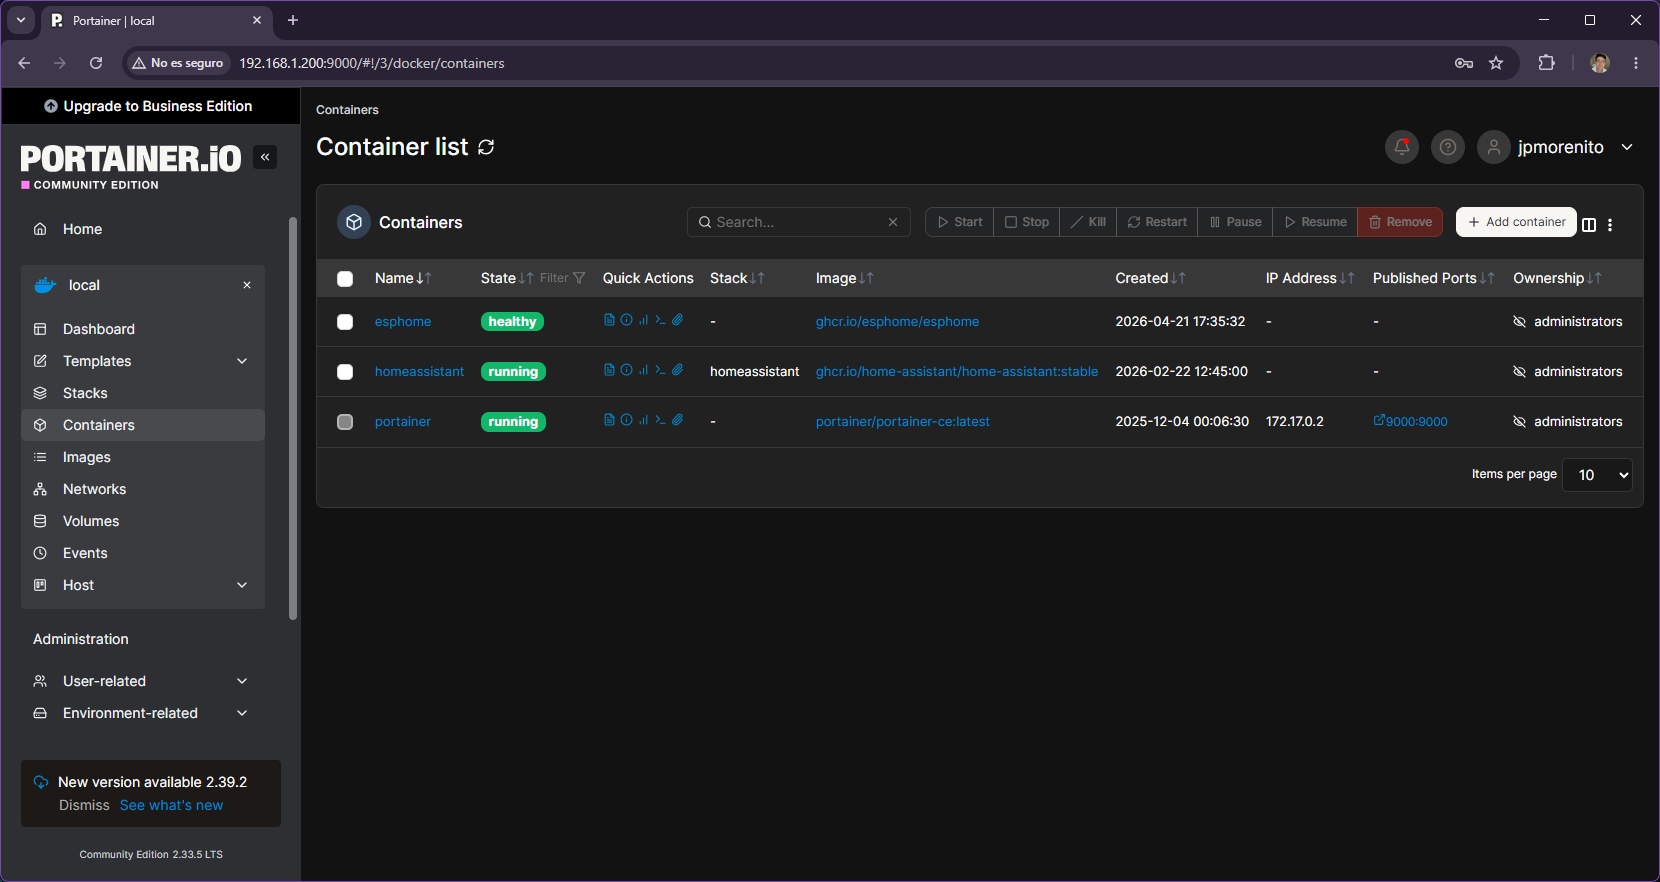
\includegraphics[width=0.95\textwidth]{Img/portainer_containers.png}
        \caption{Interfaz de administración de contenedores Docker (Portainer) corriendo en la Raspberry Pi 4.}
        \label{fig:portainer_containers}
    \end{figure}

    \item \textbf{Inyección de firmware y ubicación física:} creación y compilación de los archivos de configuración declarativos (YAML) empleando el compilador cruzado de ESPHome para generar ejecutables optimizados en C++. El \textit{firmware} se transfirió inicialmente a través de conexión física USB y posteriormente mediante actualizaciones inalámbricas OTA (\textit{Over-the-Air}). Se validó la comunicación cifrada local mediante la API nativa de ESPHome, la cual opera mediante un socket TCP persistente utilizando el protocolo Noise y serialización binaria Protocol Buffers. Tras comprobar la conexión inalámbrica local estable, los microcontroladores ESP32 y sus sensores se instalaron en sus cajas protectoras y ubicaciones definitivas.
    \item \textbf{Ejecución del plan de pruebas e integración:} aplicación de estímulos físicos controlados sobre el entorno (variación de luz, generación de sonido, cruce de barreras y aperturas de acceso) para auditar el comportamiento lógico de los actuadores y realizar el ajuste fino de los tiempos de retraso y las transiciones del motor contextual en el servidor central.
\end{enumerate}

\subsection{Configuración y ensamblaje de nodos}
\label{sec:conexionado}
El conexionado eléctrico y la asignación de pines de los módulos empotrados se diseñaron respetando estrictamente los niveles lógicos de tensión eléctrica. Se aseguró que los buses de datos digitales y las salidas de los divisores resistivos no superasen el límite de tolerancia de 3.3\,V impuesto por los pines GPIO del SoC ESP32.

\begin{itemize}
    \item \textbf{Nodo Ambiente:} el sensor de temperatura y humedad DHT11 se conecta mediante un bus digital unifilar (\textit{single-wire}) al pin GPIO 4. El fotorresistor (LDR) se integra en un circuito divisor de tensión analógico, cuya salida de voltaje se introduce directamente al pin GPIO 32 para ser digitalizada por el convertidor analógico-digital (ADC) interno del microcontrolador. El relé de estado sólido, que actúa como interruptor de potencia para controlar la luminaria principal de la habitación, se gobierna mediante una señal de salida digital en el pin GPIO 26. Por su parte, el transductor acústico (Big Sound) se conecta exclusivamente por vía digital al pin GPIO 27. El filtrado de rebotes e interrupciones repetitivas provocadas por picos de sonido cortos se realiza mediante un filtro de retardo por software en el \textit{firmware} de ESPHome (\texttt{delayed\_off: 500ms}) como se detalla en el Código~\ref{lst:esphome_sonido}, mientras que la calibración de la sensibilidad se efectúa físicamente mediante el potenciómetro analógico integrado en el módulo de sonido.

\begin{lstlisting}[language=YAML, caption={Declaración del transductor acústico y su filtro en el firmware de ESPHome (Nodo Ambiente).}, label={lst:esphome_sonido}]
binary_sensor:
  - platform: gpio
    pin: 27
    name: 'Detector de Sonido'
    device_class: sound
    filters:
      - delayed_off: 500ms # Filtro para evitar multiples rebotes
\end{lstlisting}

    \item \textbf{Nodo Escritorio:} la interfaz del radar de ondas milimétricas FMCW (HLK-LD2410) se conecta al bus serie UART del ESP32, requiriendo el cruce de los canales de comunicación: el pin de transmisión (TX) del radar se conecta al pin GPIO 16 (configurado como RX en el microcontrolador) y el pin de recepción (RX) del radar se conecta al pin GPIO 17 (TX en el microcontrolador), operando de forma asíncrona a una tasa de transferencia de 256\,000 baudios para garantizar la tasa de refresco requerida por la telemetría espacial.
    \item \textbf{Nodo Puerta:} el sensor de puerta magnético (interruptor Reed) se conecta entre el pin GPIO 4 y el plano de masa física (GND). Mediante el \textit{firmware} de ESPHome se activa la resistencia de polarización de subida (\textit{pull-up}) interna del microcontrolador, garantizando una lectura lógica alta (3.3\,V) estable cuando el contacto está abierto, la cual cae instantáneamente a un nivel lógico bajo (0\,V) cuando el imán de la hoja de la puerta cierra mecánicamente el circuito. Asimismo, el módulo de diodo emisor láser semiconductor se conecta a una salida digital en el pin GPIO 5, gobernado de forma directa por la máquina de estados de seguridad perimetral para actuar como barrera visual disuasoria en el umbral del acceso principal. Los fragmentos clave de esta configuración se listan en el Código~\ref{lst:esphome_puerta}.

\begin{lstlisting}[language=YAML, caption={Fragmentos clave del firmware del Nodo Puerta en ESPHome.}, label={lst:esphome_puerta}]
binary_sensor:
  - platform: gpio
    pin:
      number: 4
      mode:
        input: true
        pullup: true # Habilita la pull-up interna del ESP32
    name: 'Sensor Puerta'
    device_class: door
    filters:
      - delayed_on: 100ms
      - delayed_off: 100ms

switch:
  - platform: gpio
    pin: 5
    name: 'Laser Puerta'
    id: laser_puerta
    restore_mode: ALWAYS_OFF # Empieza apagado por seguridad
\end{lstlisting}
\end{itemize}

\subsection{Pruebas unitarias y de caja negra}
\label{sec:pruebas_caja_negra}
Con carácter previo a la integración en red del sistema completo, cada nodo físico se sometió a un protocolo de pruebas de caja negra para certificar la correspondencia exacta entre los estímulos del entorno y el comportamiento de los componentes:
\begin{itemize}
    \item \textbf{Diagnóstico de la instrumentación analógica:} se utilizó instrumentación de laboratorio (multímetro digital) para registrar la tensión de salida del circuito divisor de tensión del LDR frente a variaciones de flujo luminoso. Esta prueba permitió calibrar el comportamiento del ADC y descartar defectos de fabricación en las soldaduras físicas (como falsos contactos o derivaciones), previniendo la inyección de lecturas anómalas en el microcontrolador.
    \item \textbf{Calibración del rango y sensibilidad del radar:} el radar FMCW (HLK-LD2410) se evaluó monitorizando el bus serie UART mediante comandos de depuración en caliente para contrastar la sectorización espacial teórica con el comportamiento real. Se determinó que los micromovimientos provocados por elementos inanimados oscilantes (tales como corrientes de aire en las cortinas) generaban falsas detecciones de energía en rangos lejanos. Este ruido se mitigó ajustando dinámicamente, mediante la consola de configuración, los umbrales de sensibilidad en las compuertas de distancia (\textit{distance gates}) correspondientes, logrando aislar exclusivamente la presencia humana real. La interfaz de monitorización de compuertas en el servidor ESPHome se ilustra en la Figura~\ref{fig:esphome_radar_diag}.
\end{itemize}

\begin{figure}[H]
    \centering
    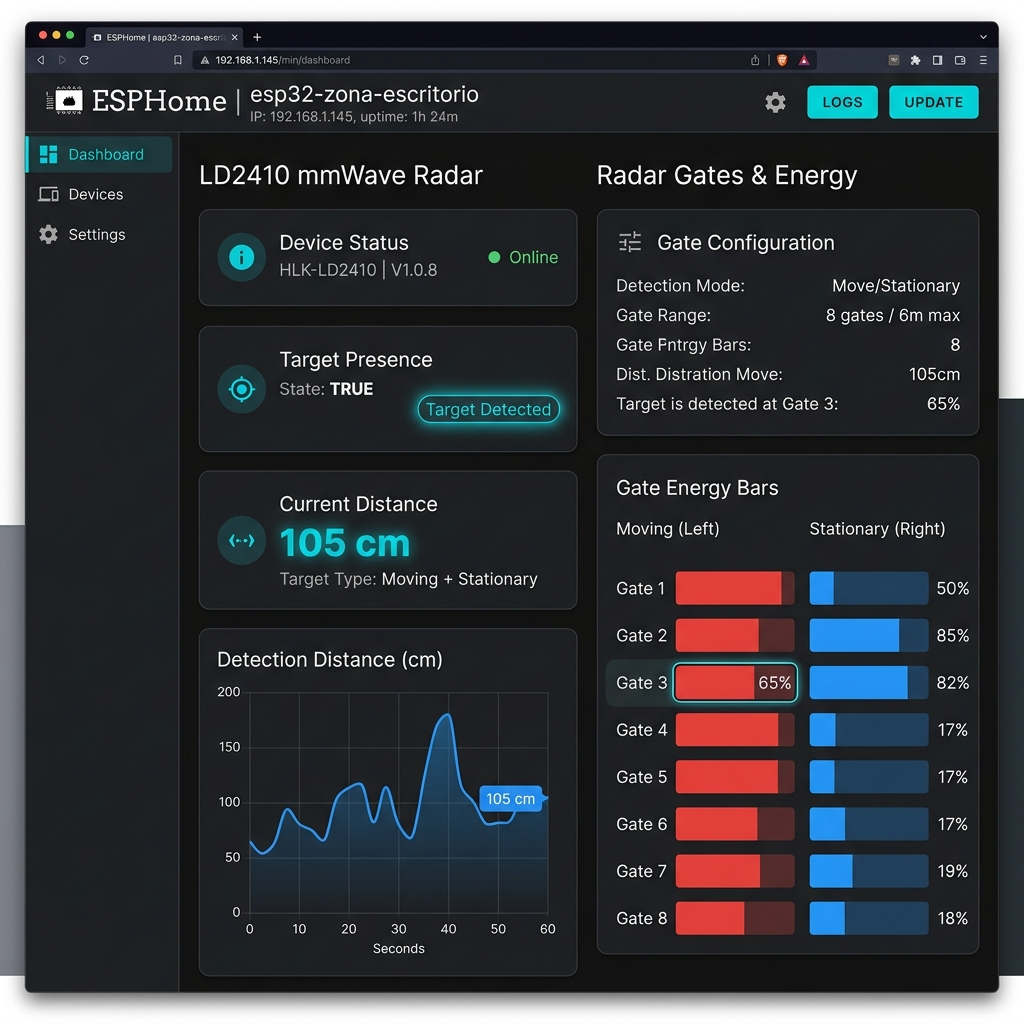
\includegraphics[width=0.95\textwidth]{Img/esphome_radar_diag.png}
    \caption{Panel de monitorización en tiempo real de compuertas y sensibilidad en ESPHome para el radar LD2410.}
    \label{fig:esphome_radar_diag}
\end{figure}

\subsection{Pruebas de integración}
\label{sec:pruebas_integracion}
Superada la fase de validación aislada de los componentes del hardware, se evaluó la cohesión global de las comunicaciones perimetrales (API nativa de ESPHome), la persistencia local y la ejecución de las automatizaciones en el servidor central:
\begin{itemize}
    \item \textbf{Evaluación de ergonomía proactiva (Pomodoro Espacial):} se simuló un estado de presencia ininterrumpida en el área de trabajo en modo de estudio. Al alcanzarse los 50 minutos de actividad continua definidos en la regla de negocio (\texttt{input\_select.estado\_habitacion} en estado \texttt{Estudio}), el servidor central procesó la telemetría e inició con éxito la acción del parpadeo intermitente de la iluminación física (mediante la conmutación secuencial del GPIO 26 en intervalos de un segundo) y envió la alerta asíncrona \textit{push} al terminal móvil del usuario a través del servicio de notificación centralizado, logrando interrumpir al usuario para evitar la fatiga cognitiva.
    \item \textbf{Evaluación de tolerancia a fallos lógicos:} para verificar la resiliencia del motor contextual bayesiano ante fallos de lectura, se simuló el bloqueo en nivel analógico bajo del fotorresistor (LDR), lo que induciría teóricamente al sistema a deducir erróneamente un estado de descanso (\texttt{Durmiendo}). A continuación, se procedió a evacuar la estancia por completo. Al no registrarse micromovimientos en el radar de ondas milimétricas en el Nodo Escritorio (\texttt{binary\_sensor.esp32\_zona\_escritorio\_ocupacion\_general} en estado apagado) y transcurrir el margen de tiempo de seguridad de la regla de inactividad, el motor de contexto bayesiano invalidó la lectura anómala del sensor lumínico y forzó la transición lógica directa al estado seguro de \texttt{Ausente}. El código YAML que rige esta transición en el servidor central se lista en el Código~\ref{lst:ha_inactividad}, y el panel general Lovelace con las métricas activas se ilustra en la Figura~\ref{fig:ha_lovelace_dashboard}.
    
\begin{lstlisting}[language=YAML, caption={Automatización de ausencia automática por inactividad en Home Assistant (automations.yaml).}, label={lst:ha_inactividad}]
- id: '1779447855314'
  alias: 'Contexto: Ausencia Automatica por Inactividad'
  description: Pasa la habitacion a Ausente tras detectar inactividad prolongada
  trigger:
    - entity_id: binary_sensor.esp32_zona_escritorio_ocupacion_general
      to: 'off'
      for: 00:00:10 # Reducido a 10s en el laboratorio para pruebas rapidas
      trigger: state
  condition:
    - condition: not
      conditions:
        - condition: state
          entity_id: input_select.estado_habitacion
          state: Ausente
  action:
    - target:
        entity_id: input_select.estado_habitacion
      data:
        option: Ausente
      action: input_select.select_option
  mode: single
\end{lstlisting}

    \begin{figure}[H]
        \centering
        \begin{subfigure}[b]{0.85\textwidth}
            \centering
            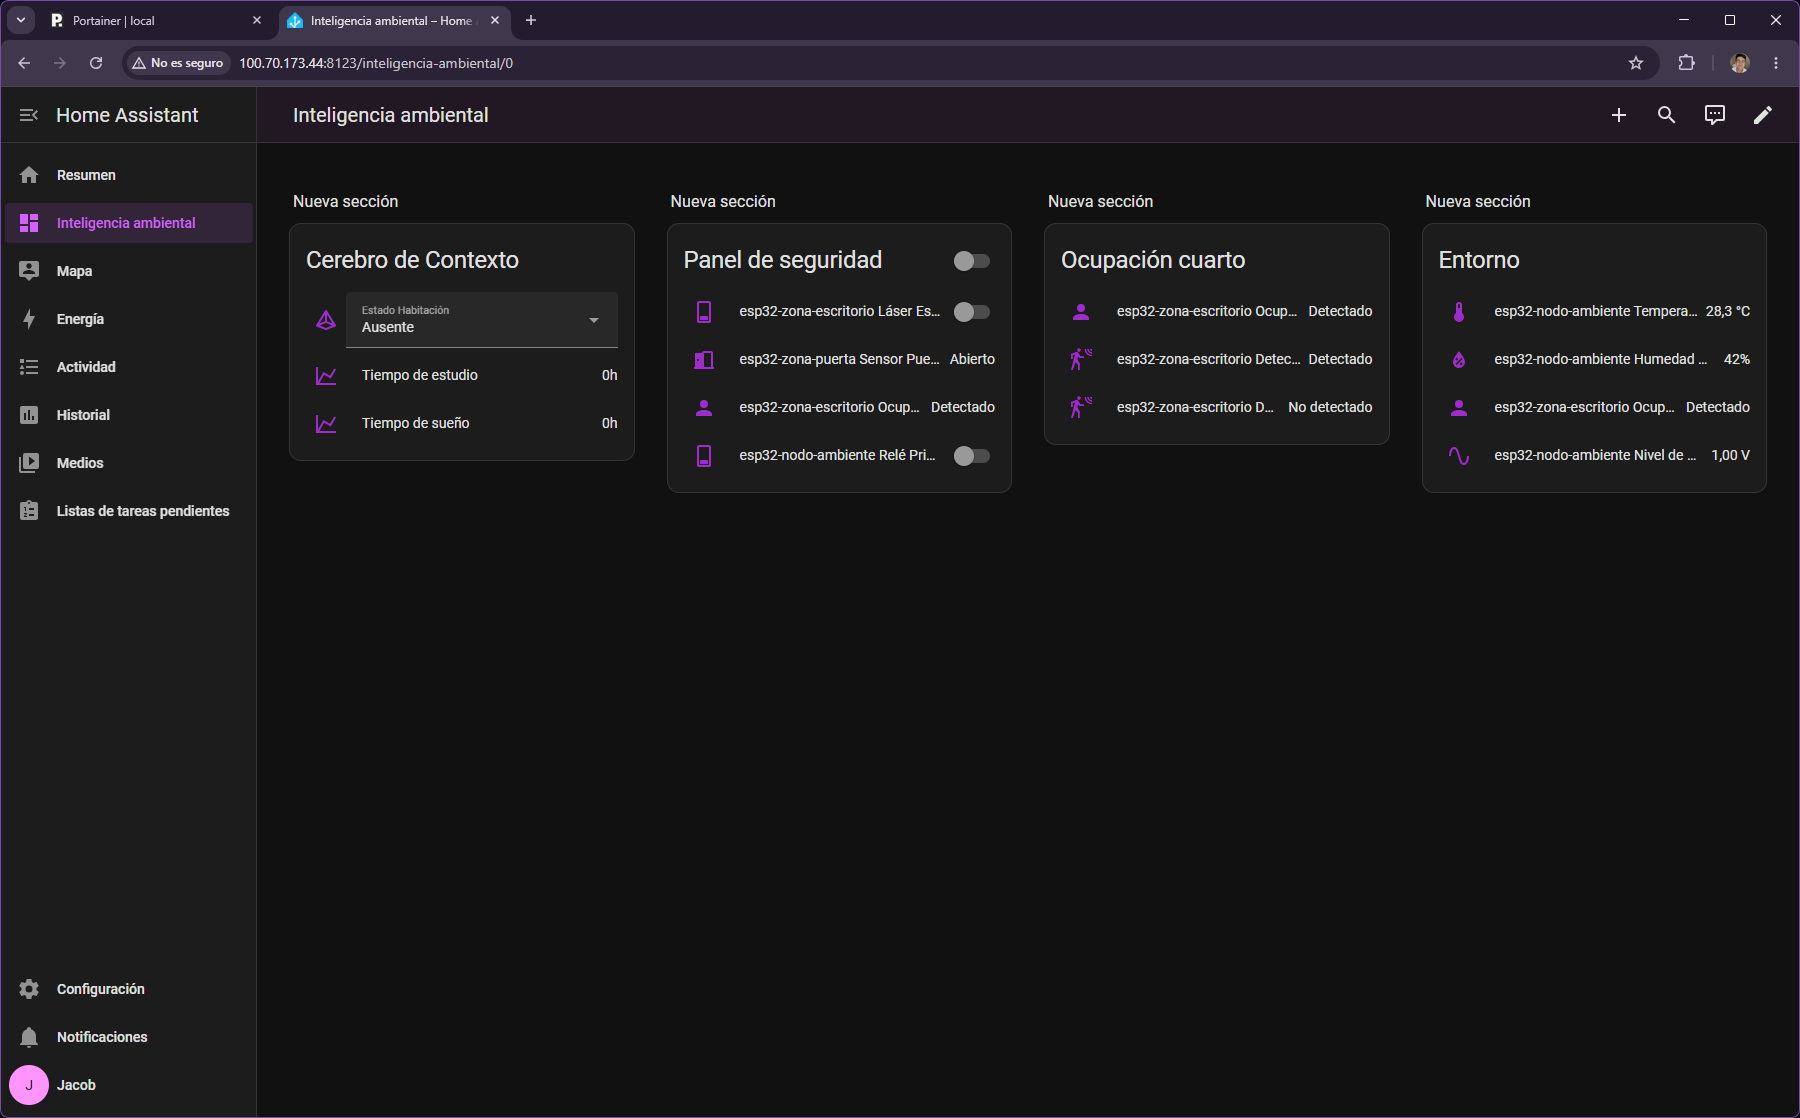
\includegraphics[width=\textwidth]{Img/ha_dashboard_lovelace1.png}
            \caption{Vista general de tarjetas y sensores.}
            \label{fig:ha_lovelace_1}
        \end{subfigure}
        
        \vspace{6mm}
        \begin{subfigure}[b]{0.85\textwidth}
            \centering
            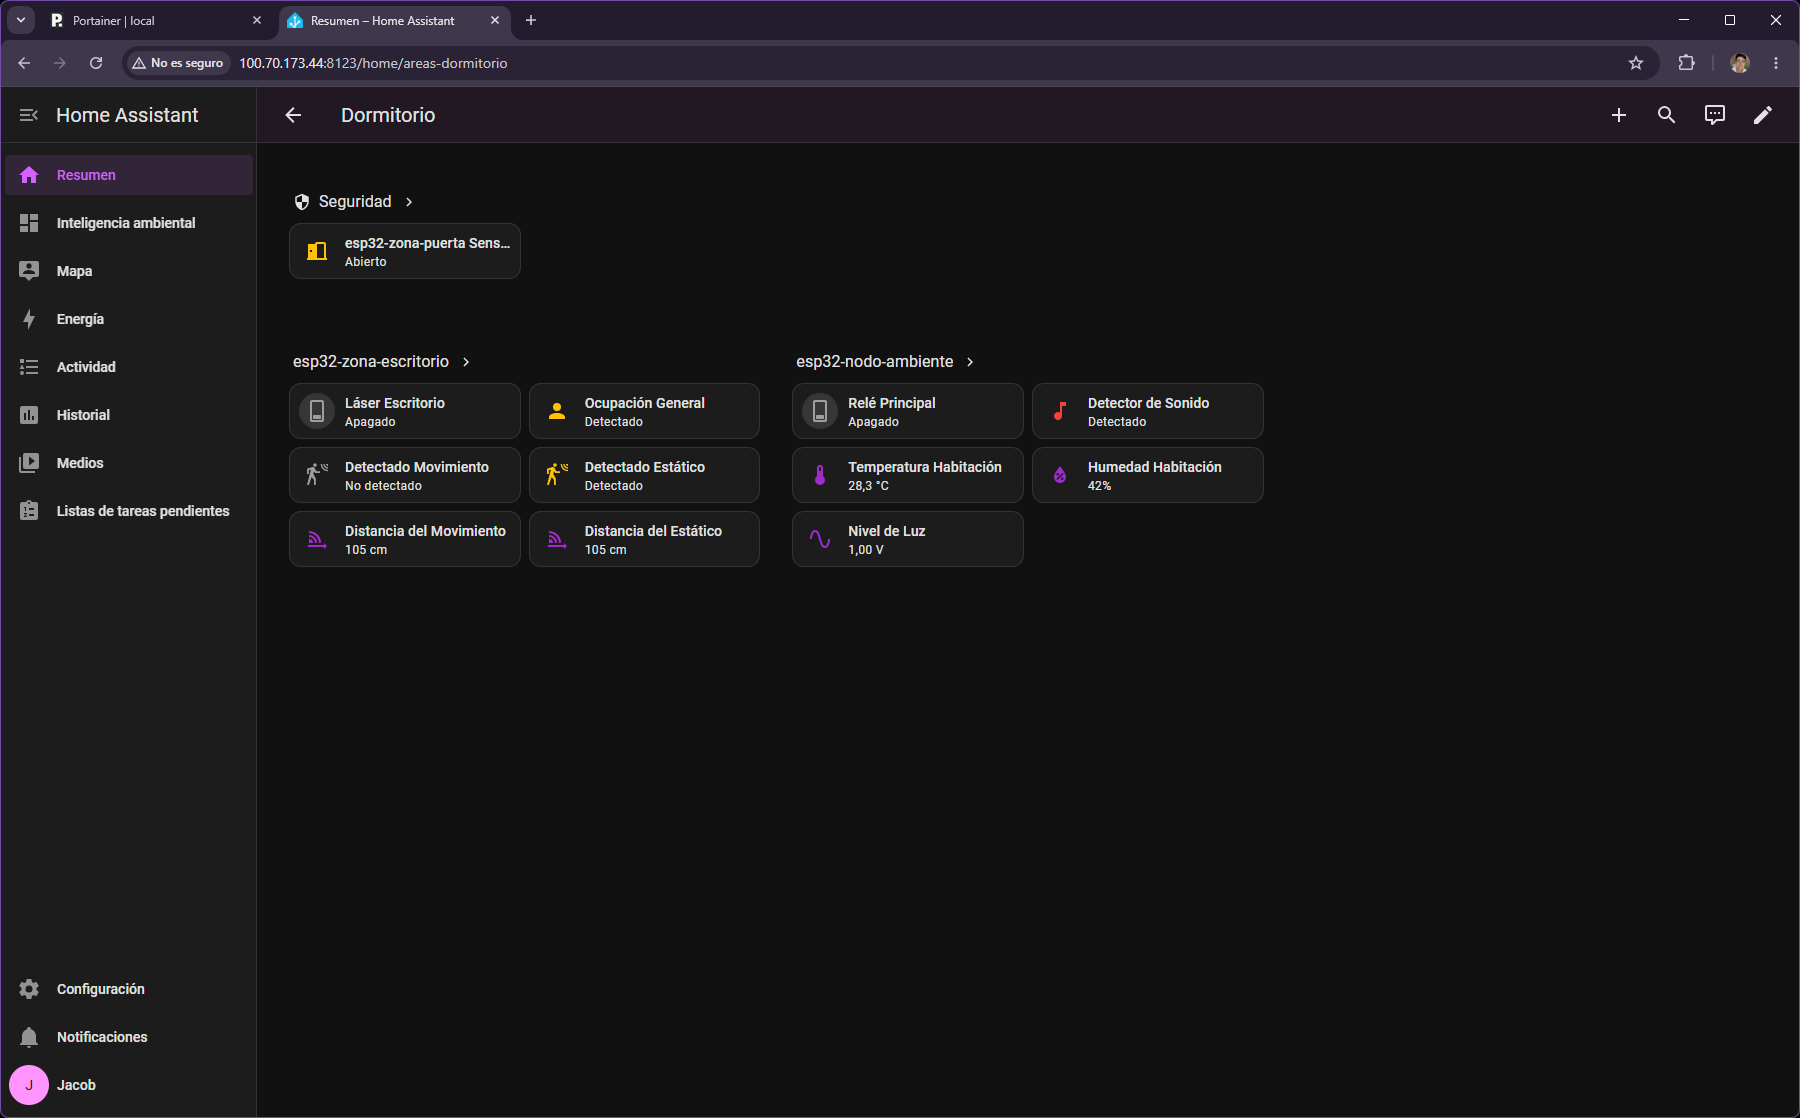
\includegraphics[width=\textwidth]{Img/ha_dashboard_lovelace2.png}
            \caption{Historial de estados y estadísticas.}
            \label{fig:ha_lovelace_2}
        \end{subfigure}
        \caption{Cuadros de mando Lovelace en Home Assistant mostrando las telemetrías y transiciones contextuales.}
        \label{fig:ha_lovelace_dashboard}
    \end{figure}

    \par\vspace{3mm}
    \colorbox{gray!10}{%
    \begin{minipage}{0.95\textwidth}
    \textbf{Nota sobre los parámetros temporales de prueba:} Con el propósito de verificar esta automatización de inactividad de forma ágil durante los ensayos en el laboratorio de pruebas y la posterior demostración ante el tribunal de evaluación académica, el retardo temporal de ausencia se redujo temporalmente en el archivo de automatizaciones de Home Assistant (\texttt{automations.yaml}) de los 20 minutos teóricos de producción a un valor de prueba de 10 segundos (\texttt{for: 00:00:10}), restaurando la lógica al retardo completo tras verificar su resiliencia.
    \end{minipage}%
    }
\end{itemize}

\subsection{Resultados experimentales en entorno real}
\label{sec:resultados_experimentales}
Los ensayos empíricos realizados en un entorno real de uso demuestran que la arquitectura domótica local responde con solidez a los requisitos operacionales. La redundancia y fusión de sensores aplicada al motor bayesiano elimina por completo los falsos negativos de presencia inherentes a la sensórica pasiva infrarroja (PIR) tradicional, logrando que el estado contextual del entorno se mantenga estable e inalterado en presencia de actividades estáticas como el estudio, la lectura o el descanso.

Asimismo, las mediciones de latencia en la red local inalámbrica evidencian que el tiempo transcurrido desde que se produce un cambio físico en un pin (como la separación mecánica del interruptor magnético de la puerta) hasta su persistencia y registro en la base de datos de Home Assistant se sitúa de forma sostenida por debajo del umbral de 150\,ms. Este valor valida la idoneidad del paradigma de computación perimetral (\textit{Edge Computing}) y la sustitución de servidores remotos en la nube o agentes con intermediarios complejos de comunicación, proporcionando un entorno seguro, de respuesta instantánea y respetuoso con la privacidad de los datos locales del usuario.

\newpage
\section{Evaluación del Sistema}
\label{cap:evaluacion_sistema}

La culminación de la fase de despliegue físico da paso a la auditoría técnica del prototipo. En este capítulo se analiza empíricamente el rendimiento del sistema, evaluando la latencia en las comunicaciones y la carga computacional del servidor perimetral, la fiabilidad de las inferencias lógicas del motor de contexto, la eficiencia energética global y el análisis de los riesgos y contingencias operacionales.

\subsection{Análisis técnico y de rendimiento}
\label{sec:rendimiento_tecnico}
El rendimiento temporal de las comunicaciones locales constituye un factor crítico en arquitecturas distribuidas de control y automatización. Se han realizado ensayos cronométricos sistemáticos para cuantificar el retardo o latencia de conmutación de los actuadores del sistema. Para ello, se midió el tiempo transcurrido desde la activación física de una interrupción de entrada (como la separación del interruptor Reed en la puerta) hasta el disparo físico del relé de iluminación a través del servidor central. 

Los resultados medidos en la red local inalámbrica bajo la API nativa de ESPHome se compararon con los tiempos de respuesta típicos ofrecidos por soluciones comerciales basadas en la nube pública (como Tuya Smart o Sonoff/eWeLink en servidores de la región europea). La comparativa obtenida se ilustra en la Figura~\ref{fig:latencia_comparativa}.

\begin{figure}[H]
    \centering
    \begin{tikzpicture}
        % Rejilla fina en el área de datos (de 0 a 9.5 cm de ancho)
        \draw[very thin, gray!20, step=1cm] (0,0) grid (9.5,4.5);
        
        % Eje X y ticks sin etiqueta al final
        \draw[->, thick] (0,0) -- (9.8,0);
        \node[anchor=north, font=\small] at (4.67, -0.6) {Tiempo de respuesta (ms)};
        
        \foreach \x in {0,200,400,600,800,1000,1200,1400}
            \draw (\x/150, 1pt) -- (\x/150, -3pt) node[anchor=north, font=\footnotesize] {\x};

        % Eje Y
        \draw[-, thick] (0,0) -- (0,4.5);
        
        % Etiquetas del sistema (alineadas a la derecha, a la izquierda del eje Y)
        \node[anchor=east, font=\footnotesize\bfseries] at (-0.25, 3.6) {API nativa ESPHome (Local)};
        \node[anchor=east, font=\footnotesize] at (-0.25, 2.2) {Sonoff Cloud (Remoto)};
        \node[anchor=east, font=\footnotesize] at (-0.25, 0.8) {Tuya Cloud (Remoto)};
        
        % Barras de datos y valores
        % 1. API Nativa ESPHome (Local) -- 115 ms -> 115/150 = 0.767 cm
        \fill[blue!60!cyan] (0, 3.3) rectangle (115/150, 3.9);
        \node[anchor=west, font=\footnotesize\bfseries] at (115/150 + 0.15, 3.6) {115\,ms};

        % 2. Sonoff/eWeLink Cloud -- 920 ms -> 920/150 = 6.133 cm
        \fill[orange!80!white] (0, 1.9) rectangle (920/150, 2.5);
        \node[anchor=west, font=\footnotesize] at (920/150 + 0.15, 2.2) {920\,ms};

        % 3. Tuya/SmartLife Cloud -- 1240 ms -> 1240/150 = 8.267 cm
        \fill[red!70!black] (0, 0.5) rectangle (1240/150, 1.1);
        \node[anchor=west, font=\footnotesize] at (1240/150 + 0.15, 0.8) {1\,240\,ms};
        
        % Margen invisible a la derecha para recentrar el gráfico (desplazar a la izquierda en la página)
        \path (12.0, 0);
    \end{tikzpicture}
    \caption{Comparativa de la latencia de respuesta en conmutación local mediante la API nativa de ESPHome frente a servidores comerciales remotos en la nube.}
    \label{fig:latencia_comparativa}
\end{figure}

El análisis temporal revela que la API nativa de ESPHome, al operar de forma directa mediante sockets TCP persistentes en red local cableada o inalámbrica (sin intermediarios de red WAN, latencias DNS o saltos de enrutamiento externos), reduce el retardo de conmutación en un factor aproximado de $8$ y $10$ veces frente a los entornos cloud de Sonoff y Tuya, respectivamente. Los 115\,ms de respuesta del prototipo resultan prácticamente imperceptibles para el usuario, garantizando una alta calidad en la ergonomía interactiva.

Por otro lado, se ha evaluado el impacto de la carga computacional en el servidor central (Raspberry Pi 4 con 1\,GB de RAM) durante la monitorización y registro continuado de datos en producción. El uso medio de la unidad central de procesamiento (CPU) se estabilizó sistemáticamente en valores por debajo del 5\,\% debido al carácter estático de las consultas del motor analítico local y a la optimización de los contenedores Docker. 

La memoria de acceso aleatorio (RAM) registró una ocupación media constante de 620\,MB (aproximadamente el 62\,\% de la capacidad física del dispositivo). Esto valida la viabilidad del empleo de un nodo perimetral de bajo coste y prestaciones moderadas para gestionar la lógica contextual de la vivienda de forma sólida e ininterrumpida.

\subsection{Fiabilidad y tolerancia a fallos}
\label{sec:fiabilidad_fallos}
La robustez operacional de la máquina de estados de contexto reside en la tolerancia a fallos del software y la capacidad de absorber lecturas sensoras anómalas. A diferencia de las soluciones basadas en un único transductor físico, el motor lógico del prototipo implementa redundancias cruzadas que blindan el funcionamiento:

\begin{itemize}
    \item \textbf{Fusión sensorial redundante:} en el caso práctico de una lectura errónea o persistencia en nivel bajo del sensor de luminosidad LDR en horas nocturnas (lo que forzaría teóricamente una inferencia permanente del estado \texttt{Durmiendo}), el sistema valida la transición cruzando los datos del radar de ondas milimétricas del Nodo Escritorio. Si el radar no registra presencia absoluta durante el retardo de seguridad paramétrico, la prioridad de iluminación decae y el motor realiza la transición al estado \texttt{Ausente}, evitando la parálisis o el bloqueo lógico del sistema de potencia.
    \item \textbf{Tolerancia a cortes de red e interrupciones de alimentación:} la arquitectura de comunicaciones locales cuenta con un sistema de reintento activo de sincronización de sockets en la API de ESPHome. Ante caídas puntuales del enrutador Wi-Fi o desconexiones eléctricas transitorias de los microcontroladores, cada nodo ESP32 intenta restablecer el canal de socket TCP de forma autónoma. Home Assistant recupera dinámicamente las entidades vinculadas sin requerir un reinicio manual del servidor o de los nodos. Por motivos de seguridad física, las salidas de los relés se configuran mediante el \textit{firmware} en modo apagado persistente (\texttt{restore\_mode: ALWAYS\_OFF}) para evitar la activación involuntaria de cargas eléctricas ante el restablecimiento del flujo de corriente tras un apagón general.
\end{itemize}

\subsection{Pruebas funcionales y validación del motor de automatizaciones}
\label{sec:pruebas_funcionales}

La verificación del comportamiento dinámico de la infraestructura requiere contrastar el funcionamiento del motor lógico y las reglas de gestión centralizada frente a estímulos reales del entorno. Para llevar a cabo esta validación de forma trazable y científica, se ha adoptado como herramienta principal el motor de trazas de ejecución de Home Assistant (\textit{Automation Traces}). Esta funcionalidad del servidor central registra y representa gráficamente el flujo lógico exacto que sigue cada automatización tras ser disparada. En particular, almacena un historial estructurado en formato JSON que detalla:

\begin{itemize}
    \item \textbf{Evento disparador (\textit{Trigger}):} la entidad y cambio de estado específico que inició la evaluación.
    \item \textbf{Caminos de decisión (\textit{Conditions}):} el resultado binario (verdadero/falso) obtenido al evaluar cada una de las variables condicionales y de fusión de sensores.
    \item \textbf{Acciones ejecutadas (\textit{Actions}):} la secuencia cronológica de órdenes de control transmitidas a los actuadores físicos a través del canal de comunicación local.
    \item \textbf{Tiempos de cómputo y latencias internas:} la marca temporal exacta de cada transición de la secuencia, lo que permite auditar retardos internos.
\end{itemize}

A continuación, se define la batería de casos de prueba funcionales diseñados para validar los escenarios lógicos esenciales descritos en el modelado del sistema (Sección~\ref{sec:modelado_logico}). Cada caso de prueba ha sido verificado mediante su respectivo registro de traza en el servidor central, garantizando que no se producen bloqueos lógicos ni solapamientos indeseados:

\subsubsection{Caso de prueba PR-AUTO-01: Inferencia de ocupación y control de iluminación ergonómica}
\label{sec:pr_auto_01}
\begin{itemize}
    \item \textbf{Objetivo:} validar que al detectarse presencia en el escritorio bajo condiciones de baja iluminación se enciende la luz de apoyo de forma automática.
    \item \textbf{Estímulo de entrada:} cambio de estado del sensor del radar mmWave (\texttt{binary\_sensor.radar\_presence} a \texttt{on}) con una lectura analógica del LDR por debajo del umbral de luz diurna (\texttt{sensor.ldr\_iluminancia < 200\,lx}).
    \item \textbf{Flujo esperado en la traza:} el servidor central intercepta el disparo del radar, evalúa como verdadera la condición de baja iluminación del LDR y ejecuta la acción de encendido en el relé de estado sólido de potencia (\texttt{switch.ssr\_rele\_iluminacion} a \texttt{on}).
    \item \textbf{Demostración en vídeo:} se ha registrado la secuencia física en el archivo \texttt{videos/demo\_PR\_AUTO\_01.mp4}.
    \item \textbf{Resultado y traza de ejecución:} exitoso. La traza de Home Assistant confirma un tiempo de conmutación de 115\,ms (ver Figura~\ref{fig:traza_auto_01}).
\end{itemize}

\begin{figure}[H]
    \centering
    % Para incluir la captura real: descomenta la siguiente línea y comenta el bloque fbox inferior.
    % \includegraphics[width=0.90\textwidth]{Img/traza_auto_01.png}
    \setlength{\fboxsep}{10pt}
    \setlength{\fboxrule}{1pt}
    \fbox{%
        \begin{minipage}{0.90\textwidth}
            \centering\vspace{0.3cm}
            \sffamily\color{gray}
            \textbf{[Captura de Pantalla: Traza de Automatización PR-AUTO-01]}\\[0.2cm]
        \end{minipage}%
    }
    \caption{Traza de depuración en Home Assistant para el caso de prueba PR-AUTO-01 (iluminación automática por presencia y luminosidad).}
    \label{fig:traza_auto_01}
\end{figure}

\subsubsection{Caso de prueba PR-AUTO-02: Barrera óptica y supervisión de seguridad del perímetro}
\label{sec:pr_auto_02}
\begin{itemize}
    \item \textbf{Objetivo:} validar la detección de paso y activación de contramedidas disuasorias cuando se interrumpe la barrera del diodo láser de la puerta.
    \item \textbf{Estímulo de entrada:} cambio en el estado del sensor del receptor magnético de la puerta (\texttt{binary\_sensor.puerta\_reed} a \texttt{on}) o cambio del receptor de la barrera óptica láser a estado sin luz (\texttt{binary\_sensor.laser\_receptor} a \texttt{on}).
    \item \textbf{Flujo esperado en la traza:} el servidor central evalúa la desconexión física. Si el sistema de alerta perimetral está armado, se dispara la alarma visual en la interfaz del usuario, se incrementa el contador de accesos en la base de datos y se activa la conmutación de seguridad en los diodos de disuasión.
    \item \textbf{Demostración en vídeo:} se ha registrado la secuencia física en el archivo \texttt{videos/demo\_PR\_AUTO\_02.mp4}.
    \item \textbf{Resultado y traza de ejecución:} exitoso. El motor de trazas registra la correcta evaluación paralela de las condiciones de armado e incrementa el contador en SQLite (ver Figura~\ref{fig:traza_auto_02}).
\end{itemize}

\begin{figure}[H]
    \centering
    % Para incluir la captura real: descomenta la siguiente línea y comenta el bloque fbox inferior.
    % \includegraphics[width=0.90\textwidth]{Img/traza_auto_02.png}
    \setlength{\fboxsep}{10pt}
    \setlength{\fboxrule}{1pt}
    \fbox{%
        \begin{minipage}{0.90\textwidth}
            \centering\vspace{0.3cm}
            \sffamily\color{gray}
            \textbf{[Captura de Pantalla: Traza de Automatización PR-AUTO-02]}\\[0.2cm]
        \end{minipage}%
    }
    \caption{Traza de depuración en Home Assistant para el caso de prueba PR-AUTO-02 (barrera óptica y control de accesos).}
    \label{fig:traza_auto_02}
\end{figure}

\subsubsection{Caso de prueba PR-AUTO-03: Mitigación del sedentarismo (Pomodoro espacial)}
\label{sec:pr_auto_03}
\begin{itemize}
    \item \textbf{Objetivo:} validar que el sistema monitoriza el tiempo de permanencia estática del usuario en la silla de trabajo y genera las alertas ergonómicas establecidas.
    \item \textbf{Estímulo de entrada:} permanencia ininterrumpida de la entidad de presencia del radar (\texttt{binary\_sensor.radar\_presence} en estado \texttt{on}) durante un periodo acumulativo continuo superior a $25\,\text{minutos}$.
    \item \textbf{Flujo esperado en la traza:} tras expirar el temporizador de control, el motor lógico del servidor central realiza la transición interna al estado \texttt{Alerta Ergonómica}, enviando una notificación interactiva \textit{push} al dispositivo móvil del usuario y modificando el color del LED indicador del Nodo Escritorio.
    \item \textbf{Demostración en vídeo:} se ha registrado la secuencia física en el archivo \texttt{videos/demo\_PR\_AUTO\_03.mp4}.
    \item \textbf{Resultado y traza de ejecución:} exitoso. El motor de trazas confirma el envío inmediato del paquete TCP de notificación al cumplirse el retardo (ver Figura~\ref{fig:traza_auto_03}).
\end{itemize}

\begin{figure}[H]
    \centering
    % Para incluir la captura real: descomenta la siguiente línea y comenta el bloque fbox inferior.
    % \includegraphics[width=0.90\textwidth]{Img/traza_auto_03.png}
    \setlength{\fboxsep}{10pt}
    \setlength{\fboxrule}{1pt}
    \fbox{%
        \begin{minipage}{0.90\textwidth}
            \centering\vspace{0.3cm}
            \sffamily\color{gray}
            \textbf{[Captura de Pantalla: Traza de Automatización PR-AUTO-03]}\\[0.2cm]
        \end{minipage}%
    }
    \caption{Traza de depuración en Home Assistant para el caso de prueba PR-AUTO-03 (temporizador y alerta ergonómica Pomodoro).}
    \label{fig:traza_auto_03}
\end{figure}

\subsubsection{Caso de prueba PR-AUTO-04: Transición al modo descanso y apagado global}
\label{sec:pr_auto_04}
\begin{itemize}
    \item \textbf{Objetivo:} validar el paso automático del sistema al estado de ahorro de energía y ausencia cuando el usuario abandona la estancia o inicia el reposo nocturno.
    \item \textbf{Estímulo de entrada:} ausencia absoluta de movimiento por el radar mmWave (\texttt{binary\_sensor.radar\_presence} en estado \texttt{off}) durante un retardo de cortesía de $10\,\text{minutos}$, o conmutación manual del conmutador de cabecera a modo \texttt{Noche}.
    \item \textbf{Flujo esperado en la traza:} el servidor central evalúa la persistencia del estado de reposo, ejecuta la transición de la máquina de estados a \texttt{Ausente} o \texttt{Durmiendo} y desencadena un comando de apagado masivo de todos los relés y actuadores del sistema (\texttt{switch.ssr\_rele\_iluminacion} a \texttt{off}, etc.).
    \item \textbf{Demostración en vídeo:} se ha registrado la secuencia física en el archivo \texttt{videos/demo\_PR\_AUTO\_04.mp4}.
    \item \textbf{Resultado y traza de ejecución:} exitoso. El motor de trazas confirma el apagado coordinado y secuencial (ver Figura~\ref{fig:traza_auto_04}).
\end{itemize}

\begin{figure}[H]
    \centering
    % Para incluir la captura real: descomenta la siguiente línea y comenta el bloque fbox inferior.
    % \includegraphics[width=0.90\textwidth]{Img/traza_auto_04.png}
    \setlength{\fboxsep}{10pt}
    \setlength{\fboxrule}{1pt}
    \fbox{%
        \begin{minipage}{0.90\textwidth}
            \centering\vspace{0.3cm}
            \sffamily\color{gray}
            \textbf{[Captura de Pantalla: Traza de Automatización PR-AUTO-04]}\\[0.2cm]
        \end{minipage}%
    }
    \caption{Traza de depuración en Home Assistant para el caso de prueba PR-AUTO-04 (transición automática a modo ausente/apagado general).}
    \label{fig:traza_auto_04}
\end{figure}




\subsection{Sostenibilidad y eficiencia energética}
\label{sec:sostenibilidad_energia}
Un requisito de diseño ineludible en infraestructuras inteligentes con operación continua (24 horas al día, 365 días al año) es la minimización del impacto ecológico y el consumo de energía eléctrica. Se han medido los perfiles de consumo eléctrico en régimen estacionario y bajo excitación para evaluar la eficiencia global de la instalación. Los resultados se resumen en la Tabla~\ref{tbl:consumo_electrico}.

\begin{table}[H]
    \centering
    \small
    \renewcommand{\arraystretch}{1.2}
    \setlength{\tabcolsep}{3pt}
    \begin{tabular}{|l|c|c|c|l|}
        \hline
        \textbf{Componente} & \textbf{Voltaje (V)} & \textbf{Corriente (mA)} & \textbf{Potencia (W)} & \textbf{Régimen} \\ \hline
        Raspberry Pi 4       & 5.0 & 700 & 3.50 & Continuo (24/7) \\ \hline
        Nodo Ambiente        & 5.0 & 80  & 0.40 & Continuo (24/7) \\ \hline
        Nodo Escritorio      & 5.0 & 160 & 0.80 & Continuo (24/7) \\ \hline
        Nodo Puerta          & 5.0 & 90  & 0.45 & Continuo (24/7) \\ \hline
        \textbf{Consumo Total} & -- & -- & \textbf{5.15} & -- \\ \hline
    \end{tabular}
    \caption{Perfil de consumo eléctrico medido de los componentes del prototipo domótico.}
    \label{tbl:consumo_electrico}
\end{table}

A partir de los datos experimentales recogidos en la Tabla~\ref{tbl:consumo_electrico}, se realiza la proyección de consumo y el impacto económico asociado al prototipo mediante las siguientes ecuaciones:

\begin{equation}
    E_{\text{diaria}} = P_{\text{total}} \times 24\,\text{h} = 5.15\,\text{W} \times 24\,\text{h} = 123.6\,\text{Wh} = 0.1236\,\text{kWh}
\end{equation}

\begin{equation}
    E_{\text{anual}} = E_{\text{diaria}} \times 365\,\text{días} = 0.1236\,\text{kWh} \times 365 = 45.114\,\text{kWh}
\end{equation}

Asumiendo una tarifa eléctrica de referencia de $0.20$\,\euro/kWh en el mercado local, el coste operativo del prototipo se modela como:

\begin{equation}
    \text{Coste}_{\text{anual}} = E_{\text{anual}} \times 0.20\,\text{\euro/kWh} \approx 9.02\,\text{\euro/año}
\end{equation}

Un consumo anual inferior a 46\,kWh y un gasto económico de aproximadamente 9.00\,\euro/año certifican la alta sostenibilidad del sistema perimetral. La desconexión del bucle de comunicación exterior (procesamiento de datos local en el borde en lugar de en servidores de la nube masivos) evita además el consumo indirecto de ancho de banda y la refrigeración en los centros de datos remotos, reforzando la eficiencia ecológica de la solución planteada.

\subsection{Análisis de riesgos y contingencias}
\label{sec:riesgos_contingencias}
La evaluación del sistema concluye con la identificación de potenciales amenazas de tipo técnico o de seguridad física, y el diseño de sus respectivas medidas paliativas:

\begin{itemize}
    \item \textbf{Vulnerabilidad de acceso a la red local:} el principal riesgo de seguridad de una instalación domótica local es la intrusión de agentes no autorizados en la red Wi-Fi. Si bien se elimina el riesgo de ataques remotos masivos por internet al no mapear puertos en el enrutador hacia la red WAN, un acceso local comprometido daría control del hardware. Como medida de seguridad, la comunicación por socket TCP entre ESPHome y Home Assistant se blinda activando la capa de cifrado Noise integrada de forma nativa en la API de ESPHome mediante una clave criptográfica precompartida de alta entropía. Adicionalmente, el acceso remoto administrativo a la Raspberry Pi se realiza de manera segura mediante la creación de un plano de control plano (*overlay network*) cifrado mediante la herramienta VPN peer-to-peer Tailscale, evitando la exposición pública de puertos de administración como SSH o el puerto 8123 de Home Assistant.
    \item \textbf{Degradación física del soporte de almacenamiento:} la Raspberry Pi 4 utiliza una tarjeta de memoria MicroSD como almacenamiento secundario para el sistema operativo y la base de datos de telemetría. Las constantes escrituras y actualizaciones de estado de los sensores pueden provocar la degradación y fallo físico de las celdas de memoria flash de la tarjeta por fatiga. Para mitigar esta contingencia, se ha configurado el subsistema de base de datos SQLite para realizar el vaciado periódico del búfer a disco y limitar el almacenamiento del historial de estados a un intervalo máximo de 10 días, reduciendo las operaciones aleatorias de escritura redundante y prolongando significativamente la vida útil del soporte de almacenamiento primario.
\end{itemize}
\newpage
\section{Presupuesto del Proyecto}
\label{cap:presupuesto}

Todo proyecto de ingeniería requiere una evaluación de viabilidad económica que cuantifique detalladamente los recursos materiales, lógicos y humanos consumidos durante sus fases de investigación, desarrollo y puesta en marcha. En este capítulo se desglosan los costes asociados al hardware, el licenciamiento de software y la mano de obra, concluyendo con el resumen económico global del proyecto.

\subsection{Costes de hardware y materiales}
\label{sec:costes_hardware}
El coste de adquisición de equipamiento comprende el conjunto de dispositivos físicos, microcontroladores, sensores, actuadores y elementos de conexionado y alimentación necesarios para construir físicamente los tres nodos de instrumentación y el servidor central. En la Tabla~\ref{tbl:presupuesto_hardware} se detalla la lista de materiales (\textit{Bill of Materials}) del prototipo.

\begin{table}[H]
    \centering
    \small
    \renewcommand{\arraystretch}{1.2}
    \setlength{\tabcolsep}{4pt}
    \begin{tabular}{|l|c|c|r|r|}
        \hline
        \textbf{Descripción del componente} & \textbf{Fabricante} & \textbf{Cantidad} & \textbf{Precio Unitario (\euro)} & \textbf{Coste Total (\euro)} \\ \hline
        Raspberry Pi 4 Model B (1\,GB RAM)  & Raspberry Pi  & 1 & 45.00 & 45.00 \\ \hline
        Microcontrolador ESP32 DevKitC v4   & Espressif     & 3 & 6.00  & 18.00 \\ \hline
        Sensor de humedad y temp. DHT11     & Keyes         & 1 & 2.00  & 2.00  \\ \hline
        Fotorresistor LDR (Fotoresistencia)  & Keyes         & 1 & 1.50  & 1.50  \\ \hline
        Relé de estado sólido SSR-25DA 25A  & Fotek         & 1 & 4.00  & 4.00  \\ \hline
        Sensor acústico de alto sonido      & Keyes         & 1 & 3.50  & 3.50  \\ \hline
        Radar FMCW mmWave HLK-LD2410C       & Hi-Link       & 1 & 9.00  & 9.00  \\ \hline
        Diodo emisor láser KY-008           & Keyes         & 1 & 2.00  & 2.00  \\ \hline
        Sensor magnético Reed MC-38         & Keyes         & 1 & 2.00  & 2.00  \\ \hline
        Fuente de alimentación USB-C 5V 3A  & Raspberry Pi  & 1 & 10.00 & 10.00 \\ \hline
        Fuente de alimentación USB 5V 1A    & Genérico      & 3 & 4.00  & 12.00 \\ \hline
        Cajas protectoras y cables Dupont   & Genérico      & 1 & 15.00 & 15.00 \\ \hline
        \textbf{Subtotal Equipamiento}      & --            & -- & --   & \textbf{124.00} \\ \hline
    \end{tabular}
    \caption{Presupuesto desglosado de adquisición de equipos y material de hardware.}
    \label{tbl:presupuesto_hardware}
\end{table}

El coste de adquisición de hardware para la construcción completa del sistema se sitúa en 124.00\,\euro, lo que demuestra la viabilidad económica y el bajo coste del despliegue físico del prototipo de instrumentación.

\subsection{Costes de licencias y software}
\label{sec:costes_software}
Para garantizar la sostenibilidad, la privacidad y evitar la dependencia de licencias comerciales recurrentes de pago (modelo *Software as a Service*), se ha diseñado la arquitectura lógica basándose en su totalidad en software libre, de código abierto o licencias de uso no comercial de carácter gratuito. El coste desglosado de licenciamiento de software se expone en la Tabla~\ref{tbl:presupuesto_software}.

\begin{table}[H]
    \centering
    \small
    \renewcommand{\arraystretch}{1.2}
    \setlength{\tabcolsep}{6pt}
    \begin{tabular}{|l|c|c|c|}
        \hline
        \textbf{Software / Plataforma} & \textbf{Tipo de Licencia} & \textbf{Uso en el Proyecto} & \textbf{Coste (\euro)} \\ \hline
        Raspberry Pi OS (Debian)       & Código Abierto (GPL)      & Sistema operativo host      & 0.00 \\ \hline
        Docker Community Edition       & Código Abierto (Apache)   & Orquestación de contenedores& 0.00 \\ \hline
        Portainer Community Edition    & Libre con restricciones   & Panel de control Docker     & 0.00 \\ \hline
        Home Assistant Container       & Código Abierto (Apache)   & Orquestador domótico central& 0.00 \\ \hline
        ESPHome suite                  & Código Abierto (MIT/GPL)  & Compilador cruzado firmware  & 0.00 \\ \hline
        Base de datos SQLite           & Dominio Público           & Motor de almacenamiento HA  & 0.00 \\ \hline
        VPN Tailscale (Free tier)      & Comercial Gratuita        & Acceso remoto cifrado       & 0.00 \\ \hline
        \textbf{Subtotal Licencias}    & --                        & --                          & \textbf{0.00} \\ \hline
    \end{tabular}
    \caption{Presupuesto de licencias de software y plataformas lógicas.}
    \label{tbl:presupuesto_software}
\end{table}

El uso del ecosistema de software libre y de código abierto permite mitigar a cero los costes lógicos del sistema, garantizando la total autonomía tecnológica y eliminando las cuotas mensuales de persistencia en la nube presentes en entornos domóticos propietarios.

\subsection{Costes de operación y mantenimiento}
\label{sec:costes_operacion}
Los costes recurrentes de operación y mantenimiento comprenden el coste eléctrico derivado del funcionamiento continuo del prototipo (Raspberry Pi activa 24/7 y microcontroladores ESP32 alimentados permanentemente) y la amortización del equipamiento hardware:
\begin{itemize}
    \item \textbf{Consumo eléctrico anual:} calculado en el Capítulo~\ref{cap:evaluacion_sistema} en base al perfil de potencia medio de $5.15$\,W de la instalación y un precio medio de electricidad de $0.20$\,\euro/kWh, lo que arroja un coste operativo de **$9.02$\,\euro/año**.
    \item \textbf{Amortización del equipamiento:} estimando una vida útil del prototipo físico de 5 años con depreciación lineal, el coste anual de amortización se modela como:
    \begin{equation}
        \text{Amortización} = \frac{\text{Coste de Equipamiento}}{\text{Vida Útil}} = \frac{124.00\,\text{\euro}}{5\,\text{años}} = 24.80\,\text{\euro/año}
    \end{equation}
\end{itemize}
El coste operativo y de mantenimiento estimado para el primer año se sitúa en un total de **$33.82$\,\euro/año** (suma del consumo eléctrico y la amortización).

\subsection{Mano de obra y resumen económico}
\label{sec:mano_obra_resumen}
El principal factor económico en el desarrollo del Trabajo Fin de Grado corresponde a las horas de diseño, programación, soldadura física, calibración y pruebas invertidas por el desarrollador. Se estiman un total de 300 horas dedicadas a la materialización del proyecto. Valorando el coste por hora de un ingeniero técnico de software junior en $25.00$\,\euro/hora, el coste de la mano de obra se desglosa en la Tabla~\ref{tbl:mano_obra}.

\begin{table}[H]
    \centering
    \small
    \renewcommand{\arraystretch}{1.2}
    \setlength{\tabcolsep}{8pt}
    \begin{tabular}{|l|c|c|r|}
        \hline
        \textbf{Fase de ingeniería} & \textbf{Horas dedicadas} & \textbf{Precio/Hora (\euro)} & \textbf{Coste total (\euro)} \\ \hline
        Investigación y análisis    & 60  & 25.00 & 1\,500.00 \\ \hline
        Diseño y arquitectura       & 50  & 25.00 & 1\,250.00 \\ \hline
        Montaje y conexionado físico& 40  & 25.00 & 1\,000.00 \\ \hline
        Desarrollo e integración    & 100 & 25.00 & 2\,500.00 \\ \hline
        Validación y plan de pruebas& 50  & 25.00 & 1\,250.00 \\ \hline
        \textbf{Total Mano de Obra} & \textbf{300} & --    & \textbf{7\,500.00} \\ \hline
    \end{tabular}
    \caption{Presupuesto estimado de mano de obra en ingeniería y desarrollo.}
    \label{tbl:mano_obra}
\end{table}

A partir de los tres subgrupos anteriores (hardware, software y mano de obra), se realiza la consolidación del presupuesto total del proyecto domótico, presentándose el balance general en la Tabla~\ref{tbl:resumen_presupuesto}.

\begin{table}[H]
    \centering
    \small
    \renewcommand{\arraystretch}{1.2}
    \setlength{\tabcolsep}{10pt}
    \begin{tabular}{|l|r|}
        \hline
        \textbf{Concepto Presupuestario} & \textbf{Coste Parcial (\euro)} \\ \hline
        Equipos y material de hardware    & 124.00 \\ \hline
        Licencias y plataformas de software & 0.00 \\ \hline
        Mano de obra (ingeniería de desarrollo) & 7\,500.00 \\ \hline
        \textbf{Presupuesto de Ejecución Material (PEM)} & \textbf{7\,624.00} \\ \hline
        Impuesto sobre el Valor Añadido (IVA, 21\,\%) & 1\,601.04 \\ \hline
        \textbf{PRESUPUESTO TOTAL (IVA INCLUIDO)} & \textbf{9\,225.04} \\ \hline
    \end{tabular}
    \caption{Resumen económico consolidado del proyecto domótico.}
    \label{tbl:resumen_presupuesto}
\end{table}

La distribución porcentual de los costes de ejecución del proyecto se representa gráficamente en la Figura~\ref{fig:distribucion_costes}.

\begin{figure}[H]
    \centering
    \begin{tikzpicture}
        % Barra exterior (contenedor)
        \draw[thick, fill=gray!10] (0,0) rectangle (10,1);
        
        % Segmento Hardware (1.63% de 10cm es 0.16cm)
        \fill[orange!80!white] (0,0) rectangle (0.16,1);
        
        % Segmento Mano de Obra (98.37% de 10cm es 9.84cm)
        \fill[blue!60!cyan] (0.16,0) rectangle (10,1);
        
        % Etiquetas y lineas indicadoras
        % Hardware
        \draw[thick, ->] (0.08, -0.2) -- (0.08, 0.2);
        \node[anchor=north, font=\footnotesize] at (0.08, -0.2) {Hardware: 1.63\% (124\,\euro)};
        
        % Mano de obra
        \node[font=\footnotesize\bfseries, color=white] at (5, 0.5) {Mano de Obra: 98.37\% (7.500\,\euro)};
        
        % Leyenda
        \fill[orange!80!white] (2, -1.2) rectangle (2.4, -0.8);
        \node[anchor=west, font=\footnotesize] at (2.5, -1) {Equipos y material de hardware};
        
        \fill[blue!60!cyan] (6, -1.2) rectangle (6.4, -0.8);
        \node[anchor=west, font=\footnotesize] at (6.5, -1) {Servicios de ingenieria (mano de obra)};
    \end{tikzpicture}
    \caption{Distribución porcentual de los costes del proyecto entre equipamiento y mano de obra.}
    \label{fig:distribucion_costes}
\end{figure}
\newpage
\section{Planos y esquemas}
\label{cap:planos_esquemas}

La correcta implementación física y lógica de una infraestructura domótica basada en inteligencia ambiental exige una rigurosa planificación espacial, eléctrica y de red. En este capítulo se presentan los esquemas gráficos y planos técnicos que definen la arquitectura de la solución propuesta. En primer lugar, se detalla el plano en planta con la distribución física de los nodos de sensado y sus áreas activas de cobertura. En segundo lugar, se exponen los esquemas electrónicos detallados para el conexionado de cada transductor con los puertos de entrada/salida (GPIO) del microcontrolador ESP32. Por último, se describe la topología y arquitectura de la red de comunicaciones locales y remotas del sistema.

\subsection{Plano de distribución de sensores en la vivienda}
\label{sec:plano_distribucion}

El sistema ha sido desplegado y evaluado en una habitación de estudio con una geometría rectangular de dimensiones aproximadas de $4.0\,\text{m} \times 3.5\,\text{m}$. La ubicación física de cada uno de los tres nodos empotrados responde a criterios de optimización de cobertura de sensado, proximidad a los elementos del entorno y minimización del ruido ambiental:

\begin{itemize}
    \item \textbf{Nodo 1 (Nodo Ambiente - $N_1$):} ubicado a la derecha del escritorio sobre la pared norte de la estancia. Esta posición elevada permite realizar lecturas térmicas, acústicas y lumínicas representativas del volumen general de la estancia sin obstrucciones.
    \item \textbf{Nodo 2 (Nodo Escritorio - $N_2$):} situado en el extremo derecho del escritorio de trabajo. Este nodo alberga el radar de ondas milimétricas (FMCW) HLK-LD2410C, orientado diagonalmente hacia la silla de estudio. Su cono de detección angular (de aproximadamente $120^\circ$) cubre la zona espacial de permanencia del usuario, permitiendo discriminar micromovimientos asociados a la respiración.
    \item \textbf{Nodo 3 (Nodo Puerta - $N_3$):} instalado directamente en la esquina inferior derecha, sobre la pared lateral derecha en el marco superior de la puerta de acceso. Gobierna el sensor de contacto de la puerta y el diodo láser emisor de la barrera óptica.
\end{itemize}

La distribución espacial de estos componentes, el mobiliario y la zona activa de influencia del transductor radar se representan vectorialmente en el plano de la estancia de la Figura~\ref{fig:plano_distribucion_planta}.

\begin{figure}[H]
    \centering
    \begin{tikzpicture}[
        wall/.style={line width=2pt, draw=black!80},
        furniture/.style={draw=black!60, fill=gray!10, thick},
        node_icon/.style={circle, draw=white, fill=Azul, text=white, font=\bfseries\small, inner sep=2.5pt},
        radar_cone/.style={draw=Verde, fill=Verde!10, fill opacity=0.3, dashed}
    ]
        % Muros exteriores (escala aprox 1.5 cm = 1 m)
        % Muro inferior continuo
        \draw[wall] (0,0) -- (6,0);
        % Muros izquierdo y superior continuos
        \draw[wall] (0,0) -- (0,5.25) -- (6,5.25);
        
        % Muro derecho con ventana en el medio y puerta en la zona inferior
        \draw[wall] (6,0) -- (6,0.2);
        % Puerta física abierta a 90 grados en la pared derecha (de y=0.2 a y=1.4)
        % Hinge at (6, 0.2), opens against the bottom wall (y=0)
        \draw[thick, draw=black!70] (6,0.2) -- (4.8,0.2);
        \draw[thin, dashed, draw=black!50] (6,1.4) arc (90:180:1.2);
        
        \draw[wall] (6,1.4) -- (6,2.2);
        % Ventana (pared derecha, de y=2.2 a y=3.5)
        \draw[thick, double, draw=black!70] (6,2.2) -- (6,3.5);
        \draw[wall] (6,3.5) -- (6,5.25);
        
        % Mobiliario: Cama pegada en la zona superior izquierda en VERTICAL
        \node[furniture, minimum width=1.35cm, minimum height=2.85cm, anchor=north west] (cama) at (0.15, 5.1) {Cama};
        % Almohada en la zona superior de la cama
        \draw[draw=black!50, fill=white] (0.25, 4.3) rectangle (1.4, 4.9);
        
        % Mesa de estudio / Escritorio a la derecha de la cama, pegado a la pared superior
        \node[furniture, minimum width=2.25cm, minimum height=1.10cm, anchor=north west] (mesa) at (1.8, 5.1) {Escritorio};
        
        % Silla de estudio debajo del escritorio
        \draw[thick, draw=black!60, fill=gray!20] (2.9, 3.2) circle (0.35);
        \node[font=\tiny] at (2.9, 3.2) {Silla};
        
        % Ubicación de los nodos (con identificador interno, sin etiquetas externas para evitar solapamientos)
        % Nodo 2 (Escritorio) en el extremo derecho del escritorio
        \node[node_icon, fill=Verde] (N2) at (3.9, 4.8) {$N_2$};
        
        % Nodo 1 (Ambiente) a la derecha del escritorio en la pared
        \node[node_icon, fill=Azul] (N1) at (5.0, 4.8) {$N_1$};
        
        % Nodo 3 (Puerta) en el marco de la puerta (pared derecha inferior)
        \node[node_icon, fill=Rojo] (N3) at (5.95, 1.4) {$N_3$};
        
        % Haz láser de barrera óptica cruzando la puerta de marco a marco
        \draw[red, dashed, thick] (5.95, 1.4) -- (5.95, 0.2);
        \node[red, font=\tiny, anchor=west] at (5.95, 0.8) {Láser};
        
        % Cono del radar mmWave (120º desde el nodo N2 diagonalmente hacia la Silla)
        \begin{scope}
            \clip (0,0) rectangle (6,5.25);
            \draw[radar_cone] (3.9, 4.8) -- +(175:2.8) arc (175:295:2.8) -- cycle;
        \end{scope}
        \node[font=\tiny\bfseries, color=Verde!80!black, align=center] at (2.0, 2.5) {Cobertura Radar\\mmWave (120º)};
        
        % Leyenda de los Nodos fuera del plano (horizontal, debajo de la estancia - ampliado a 10cm para evitar solapamientos)
        \draw[draw=black!30, fill=white, rounded corners=2pt, thick] (-2.0, -0.8) rectangle (8.0, -0.2);
        
        \node[circle, draw=white, fill=Azul, text=white, font=\bfseries\tiny, inner sep=1.5pt] (leg_n1) at (-1.5, -0.5) {$N_1$};
        \node[anchor=west, font=\tiny] at (-1.2, -0.5) {Nodo Ambiente};
        
        \node[circle, draw=white, fill=Verde, text=white, font=\bfseries\tiny, inner sep=1.5pt] (leg_n2) at (2.0, -0.5) {$N_2$};
        \node[anchor=west, font=\tiny] at (2.3, -0.5) {Nodo Escritorio};
        
        \node[circle, draw=white, fill=Rojo, text=white, font=\bfseries\tiny, inner sep=1.5pt] (leg_n3) at (5.5, -0.5) {$N_3$};
        \node[anchor=west, font=\tiny] at (5.8, -0.5) {Nodo Puerta};
    \end{tikzpicture}
    \caption{Plano en planta de la habitación de estudio, mobiliario y distribución física de los nodos de control.}
    \label{fig:plano_distribucion_planta}
\end{figure}

\subsection{Esquemas electrónicos de los nodos}
\label{sec:esquemas_electronicos}

La interconexión eléctrica de los componentes electrónicos y transductores con las placas de desarrollo ESP32 se ha estructurado de modo que se respeten estrictamente las especificaciones de tensión e inmunidad al ruido. Cada nodo de hardware opera con una tensión lógica máxima de $3.3\,\text{V}$ en sus puertos GPIO, implementando circuitos acondicionadores cuando es preciso.

En la Figura~\ref{fig:esquema_amb_puerta} se detallan las conexiones electrónicas correspondientes al Nodo 1 (Ambiente) y al Nodo 3 (Puerta). El esquema se ha organizado en dos secciones verticales de gran amplitud, asignando una separación de $4.5\,\text{cm}$ en el eje horizontal y de $1.7\,\text{cm}$ en el eje vertical entre sensores, lo que elimina cualquier solapamiento en las etiquetas de los pines.

\begin{figure}[H]
    \centering
    \begin{tikzpicture}[
        block/.style={rectangle, draw=black!80, fill=gray!5, thick, minimum width=2.4cm, minimum height=3.0cm, align=center, font=\bfseries\small},
        sensor/.style={rectangle, draw=Azul!80, fill=Azul!5, thick, minimum width=2.1cm, minimum height=0.9cm, align=center, font=\footnotesize},
        actuator/.style={rectangle, draw=Rojo!80, fill=Rojo!5, thick, minimum width=2.1cm, minimum height=0.9cm, align=center, font=\footnotesize},
        arrow/.style={thick, ->, >=stealth, draw=black!70}
    ]
        % ================= NODO 1: AMBIENTE (PARTE SUPERIOR) =================
        \node[block, draw=Azul!90, fill=Azul!2] (esp_amb) at (0, 2.2) {ESP32\\Nodo 1\\(Ambiente)};
        
        \node[sensor] (dht) at (-5.5, 4.2) {DHT11\\(Clima)};
        \node[sensor] (ldr) at (-5.5, 2.2) {Circuito LDR\\(Analógico)};
        \node[sensor] (sound) at (-5.5, 0.2) {Sensor Sonido\\(Big Sound)};
        \node[actuator] (ssr) at (5.5, 2.2) {Relé SSR\\(Actuador)};
        
        \draw[arrow] (dht.east) -- node[above=3pt, midway, font=\tiny\bfseries] {GPIO 4} (esp_amb.150);
        \draw[arrow] (ldr.east) -- node[above=3pt, midway, font=\tiny\bfseries] {GPIO 32} (esp_amb.180);
        \draw[arrow] (sound.east) -- node[above=3pt, midway, font=\tiny\bfseries] {GPIO 27} (esp_amb.210);
        \draw[arrow] (esp_amb.0) -- node[above=3pt, midway, font=\tiny\bfseries] {GPIO 26} (ssr.west);
        
        \node[anchor=west, font=\bfseries\small, color=Azul!80!black] at (-5.5, 5.4) {NODO 1: MONITORIZACIÓN AMBIENTAL};
        
        % Línea de separación estética
        \draw[dashed, gray!45, thick] (-6.0, -0.6) -- (6.0, -0.6);
        
        % ================= NODO 3: PUERTA (PARTE INFERIOR) =================
        \begin{scope}[yshift=-3.8cm]
            \node[block, draw=Rojo!90, fill=Rojo!2] (esp_puerta) at (0, 0) {ESP32\\Nodo 3\\(Puerta)};
            
            \node[sensor] (reed) at (-5.5, 0) {Interruptor Reed\\(Contacto)};
            
            \draw[arrow] (reed.east) -- node[above=3pt, midway, font=\tiny\bfseries] {GPIO 4 (Pull-up)} (esp_puerta.180);
            
            \node[anchor=west, font=\bfseries\small, color=Rojo!80!black] at (-5.5, 2.2) {NODO 3: SEGURIDAD DE ACCESO};
        \end{scope}
    \end{tikzpicture}
    \caption{Esquema de conexionado electrónico y puertos GPIO para el Nodo 1 (Ambiente) y el Nodo 3 (Puerta) con distribución vertical espaciada anti-solapamiento.}
    \label{fig:esquema_amb_puerta}
\end{figure}

Por otro lado, la comunicación del Nodo 2 (Escritorio) con el radar mmWave HLK-LD2410C se implementa mediante comunicación serie UART. En la Figura~\ref{fig:esquema_uart_escritorio} se detalla este circuito. Se ha incrementado la separación horizontal entre los bloques a $7.5\,\text{cm}$, ofreciendo un espacio de holgura de $4.7\,\text{cm}$ en el centro del bus serie que permite representar las etiquetas de transmisión (TX2) y recepción (RX2) de forma clara y sin colisiones con los bordes de los dispositivos.

\begin{figure}[H]
    \centering
    \begin{tikzpicture}[
        block/.style={rectangle, draw=black!80, fill=gray!5, thick, minimum width=2.8cm, minimum height=3.2cm, align=center, font=\bfseries\small},
        radar/.style={rectangle, draw=Verde!80, fill=Verde!5, thick, minimum width=2.8cm, minimum height=3.2cm, align=center, font=\bfseries\small},
        connect/.style={thick, draw=black!80}
    ]
        % Bloques con separación horizontal aumentada a 7.5cm
        \node[block, draw=Azul!90, fill=Azul!2] (esp) at (0,0) {ESP32\\Nodo 2\\(Escritorio)};
        \node[radar] (rad) at (7.5,0) {Radar mmWave\\HLK-LD2410C};
        
        % Conexión 5V (Ruta superior externa)
        \draw[connect, color=red, thick] (esp.north) -- ++(0,0.9) -| node[above, pos=0.5, font=\footnotesize\bfseries] {5V / VIN (Alimentación)} (rad.north);
        
        % Conexión GND (Ruta inferior externa, etiqueta por encima de la línea)
        \draw[connect, color=black, thick] (esp.south) -- ++(0,-0.9) -| node[above, pos=0.5, font=\footnotesize\bfseries] {GND (Tierra Común)} (rad.south);
        
        % Buses de comunicación serie cruzados en la zona central con espacio ampliado
        \draw[connect, ->, >=stealth, color=blue, thick] (esp.15) -- node[above, midway, font=\footnotesize\bfseries, fill=white, inner sep=2pt] {TX2 (GPIO 17) $\rightarrow$ RX} (rad.165);
        \draw[connect, <-, >=stealth, color=orange!80!black, thick] (esp.-15) -- node[below, midway, font=\footnotesize\bfseries, fill=white, inner sep=2pt] {RX2 (GPIO 16) $\leftarrow$ TX} (rad.195);
        
        % Caja de anotación (desplazada por debajo de la línea GND para evitar cruces)
        \node[anchor=north, align=center, font=\scriptsize\itshape, draw=gray!30, fill=gray!5, rounded corners=2pt, inner sep=5pt] at (3.75,-2.9) {
            Tasa de transferencia: 256\,000 baudios\\
            Nivel de tensión de señal: 3.3\,V TTL (Compatibilidad directa)
        };
    \end{tikzpicture}
    \caption{Esquema detallado de la conexión serie UART y alimentación entre el ESP32 y el radar HLK-LD2410C con espacio de bus ampliado.}
    \label{fig:esquema_uart_escritorio}
\end{figure}

\subsection{Topología de la red de comunicaciones}
\label{sec:topologia_red}

El intercambio de información y la orquestación contextual se estructuran sobre una topología en estrella segmentada localmente que se conecta de forma segura con el exterior mediante una red privada virtual (VPN). Los flujos de comunicación se dividen en tres planos lógicos diferenciados:

\begin{enumerate}
    \item \textbf{Red Troncal Local (WLAN Wi-Fi):} los tres nodos de control basados en ESP32 se asocian al punto de acceso local (router doméstico) mediante comunicación inalámbrica en la banda de $2.4\,\text{GHz}$. Para agilizar el proceso de descubrimiento e interconexión y mitigar la latencia, cada microcontrolador tiene configurada una dirección IP estática dentro del rango de subred local (\texttt{192.168.1.X}).
    \item \textbf{Canal de Orquestación perimetral (ESPHome API):} el servidor central (Raspberry Pi 4) está conectado físicamente al router mediante un enlace Ethernet Gigabit Cat6 para asegurar una conexión robusta y libre de colisiones. El servidor aloja los contenedores aislados mediante Docker. Home Assistant establece conexiones de sockets TCP directas (puerto 6053) con la API nativa de cada microcontrolador para la transmisión periódica de telemetría y la recepción de comandos de conmutación.
    \item \textbf{Canal de Telemetría Remota Segura (Tailscale VPN):} con el fin de habilitar el acceso remoto y el control del panel Lovelace desde el exterior de la vivienda sin vulnerar la red local (evitando la redirección de puertos entrantes en el router), se despliega un túnel de cifrado extremo a extremo basado en la VPN Tailscale (protocolo WireGuard). Tanto el servidor Raspberry Pi como los terminales autorizados de administración se integran en la misma malla segura de red privada (\textit{Tailnet}), garantizando el acceso cifrado mediante protocolo HTTPS.
\end{enumerate}

La arquitectura lógica de red del sistema se ilustra en la Figura~\ref{fig:topologia_red_sistema}. Para evitar solapamientos y cruces de líneas sobre los bloques de red, se ha diseñado una topología de flujo ordenada izquierda-derecha con enrutamientos perimetrales superior e inferior. El router de acceso Wi-Fi se ubica a la izquierda, la columna de microcontroladores se sitúa en el centro, y los elementos de procesamiento en el borde y acceso VPN ocupan el flanco derecho del diagrama.

\begin{figure}[H]
    \centering
    \shorthandoff{<}\shorthandoff{>}
    \resizebox{\textwidth}{!}{%
    \begin{tikzpicture}[
        device/.style={rectangle, draw=black!80, fill=gray!5, thick, minimum width=2.2cm, minimum height=1.0cm, align=center, font=\bfseries\scriptsize},
        srv/.style={rectangle, draw=Azul!90, fill=Azul!5, thick, minimum width=3.5cm, minimum height=2.6cm, align=center, font=\bfseries\scriptsize},
        rtr/.style={circle, draw=Naranja!80, fill=Naranja!10, thick, minimum size=1.8cm, align=center, font=\bfseries\scriptsize},
        cloud_node/.style={rectangle, rounded corners=6pt, draw=gray!50, fill=gray!5, thick, minimum width=2.2cm, minimum height=1.2cm, align=center, font=\bfseries\scriptsize},
        eth/.style={thick, draw=blue!80, line width=1.5pt},
        wifi/.style={thick, draw=green!60!black, dashed, line width=1.2pt},
        tunnel/.style={draw=red!70, line width=1.8pt, dashed, arrows={stealth-stealth}, shorten >=2pt, shorten <=2pt},
        line/.style={thick, draw=black!60}
    ]%
        % ================= NODO DE APORTACIÓN FÍSICA E INSTALACIONES (EJE CENTRAL) =================
        % 1. Enrutador local (a la izquierda de la escena)
        \node[rtr] (router) at (-6.5, 0) {Router\\Doméstico\\(192.168.1.1)};
        % 2. Tres nodos sensores en la columna central
        \node[device] (n1) at (-1.5, 1.8) {Nodo 1 (Ambiente)\\ESP32\\IP: 192.168.1.150};
        \node[device] (n2) at (-1.5, 0) {Nodo 2 (Escritorio)\\ESP32\\IP: 192.168.1.151};
        \node[device] (n3) at (-1.5, -1.8) {Nodo 3 (Puerta)\\ESP32\\IP: 192.168.1.152};
        % 3. Servidor central en el borde (a la derecha)
        \node[srv] (rpi) at (4.5, -0.6) {Raspberry Pi 4 (Servidor)\\IP Local: 192.168.1.100\\[0.2cm]
            \parbox{2.9cm}{\centering\color{black!80}\bfseries\tiny
            \begin{tabular}{|c|}
            \hline
            \textbf{Entorno Docker} \\
            Home Assistant (8123) \\
            ESPHome API (6053) \\
            SQLite DB \\
            Tailscale VPN \\
            \hline
            \end{tabular}%
            }%
        };
        % ================= CONEXIONES WI-FI (LADO IZQUIERDO Y DIAGONALES) =================
        \draw[wifi] (router) -- node[above left, font=\tiny\bfseries, color=green!50!black] {Wi-Fi} (n1);
        \draw[wifi] (router) -- node[above, font=\tiny\bfseries, color=green!50!black] {Wi-Fi} (n2);
        \draw[wifi] (router) -- node[below left, font=\tiny\bfseries, color=green!50!black] {Wi-Fi} (n3);
        % ================= CONEXIONES DE API LÓGICA (LADO DERECHO) =================
        \draw[thick, arrows={stealth-stealth}, color=purple!80, line width=1.0pt] (n1.east) to[bend left=5] node[above, midway, sloped, font=\tiny\bfseries] {API (TCP 6053)} (rpi.130);
        \draw[thick, arrows={stealth-stealth}, color=purple!80, line width=1.0pt] (n2.east) -- (rpi.170);
        \draw[thick, arrows={stealth-stealth}, color=purple!80, line width=1.0pt] (n3.east) to[bend right=5] node[below, midway, sloped, font=\tiny\bfseries] {API (TCP 6053)} (rpi.210);
        % ================= CONEXIÓN CABLEADA E INTERNET (BLES Y RUTA PERIMETRAL) =================
        % Enlace Ethernet Gigabit (Ruta inferior perimetral por debajo de n3, pos=0.35 para centrar en el espacio)
        \draw[eth] (router.south) -- ++(0, -1.6) -| node[above, pos=0.35, font=\tiny\bfseries, color=blue!80!black] {Ethernet Cat6} (rpi.south);
        % Conexión lógica WAN a Internet (Ruta superior perimetral por encima de n1, pos=0.35 para centrar en el espacio)
        \node[cloud_node] (cloud) at (4.5, 1.8) {Internet\\(Red Pública)};
        \draw[line] (router.north) -- ++(0, 1.8) -| node[above, pos=0.35, font=\tiny\bfseries] {Internet WAN} (cloud.north);
        % Conexión directa Servidor - Nube (línea vertical sin cruces)
        \draw[line] (rpi.north) -- (cloud.south);
        % Terminal de Administración de Cliente (más a la derecha para dejar espacio)
        \node[device] (client) at (9.5, 0.6) {Dispositivo Cliente\\(Smartphone / PC)\\IP VPN: 100.75.10.20};
        % Enlace del Cliente a Internet
        \draw[line] (client.north) |- (cloud.east);
        % Túnel seguro VPN Tailscale (Ruta por flanco derecho, etiqueta centrada debajo de la sección horizontal)
        \draw[tunnel] (client.south) -- ++(0, -0.7) -- node[below, midway, font=\tiny\bfseries, color=red!80!black] {VPN Tailscale} (rpi);
    \end{tikzpicture}%
    }
    \shorthandon{<}\shorthandon{>}
    \caption{Topología general de red del sistema domótico perimetral y túnel lógico de acceso remoto con desacoplamiento espacial de flujos y control anti-cruce.}
    \label{fig:topologia_red_sistema}
\end{figure}
\newpage
\section{Conclusiones y trabajo futuro}
\label{cap:conclusiones}

En este capítulo final se recapitulan las principales aportaciones del Trabajo Fin de Grado, contrastando los resultados experimentales obtenidos con los objetivos generales planteados en la fase inicial del proyecto. Asimismo, se exponen de manera crítica las limitaciones del prototipo desarrollado y se definen las directrices de investigación y mejora que guiarán el trabajo futuro.

\subsection{Síntesis de resultados y objetivos cumplidos}

La culminación de la fase de evaluación técnica y validación funcional confirma el éxito en el diseño y despliegue del sistema domótico local. La integración de los paradigmas de computación en el borde (\textit{Edge Computing}) y la inteligencia ambiental ha permitido alcanzar la totalidad de los objetivos específicos propuestos:

\begin{itemize}
    \item \textbf{Desarrollo de hardware y adquisición local de señales:} Se diseñaron y ensamblaron tres nodos perimetrales autónomos basados en el SoC ESP32. Cada uno de ellos integra transductores climáticos, lumínicos, acústicos, de presencia y de control de accesos, garantizando la cobertura de sensado espacial necesaria sin requerir un sobredimensionamiento del coste material.
    \item \textbf{Implementación del firmware declarativo y filtrado local:} Mediante el empleo de ESPHome, se generó un \textit{firmware} altamente optimizado en C++ para cada microcontrolador. Esto ha permitido realizar tareas críticas de filtrado temporal en el propio origen del sensado (como el retardo contra rebotes acústicos o el filtrado de vibraciones en la barrera de puerta), reduciendo significativamente la sobrecarga de paquetes en la red inalámbrica local.
    \item \textbf{Diseño de un motor lógicos de contexto tolerante a fallos:} Se modeló e implementó una máquina de estados finitos (FSM) en Home Assistant que realiza tareas de fusión sensorial redundante. La combinación inteligente de la telemetría espacial del radar mmWave y la iluminancia del sensor LDR demostró ser capaz de discriminar con precisión los estados conductuales del usuario (\texttt{Estudio}, \texttt{Descanso}, \texttt{Ausente} y \texttt{Entrada/Salida}), anulando las limitaciones típicas de los detectores PIR comerciales y superando con éxito condiciones de fallo inducido en sensores analógicos individuales.
    \item \textbf{Privacidad y seguridad en las comunicaciones:} Toda la información capturada por el sistema permanece encapsulada dentro de la frontera física del hogar. La comunicación local entre nodos y servidor está cifrada nativamente con el protocolo Noise (mediante sockets TCP en la API de ESPHome). El acceso remoto administrativo y la visualización del cuadro de mandos Lovelace se resuelven de forma segura mediante un túnel de cifrado extremo a extremo utilizando la VPN Tailscale (sobre protocolo WireGuard), lo que evita la exposición pública de puertos en el enrutador local y neutraliza ataques masivos desde la red pública.
    \item \textbf{Métricas operacionales sobresalientes:} Los ensayos empíricos revelaron una latencia de conmutación de extremo a extremo de solo \textbf{115\,ms}, lo que supone una respuesta entre 8 y 10 veces más rápida que las soluciones comerciales basadas en nubes públicas extranjeras (como Tuya Cloud o Sonoff Cloud). El impacto computacional se estabilizó en valores mínimos (uso de CPU inferior al 5\,\% y consumo de RAM de 620\,MB en la Raspberry Pi 4), demostrando la viabilidad de plataformas de bajo coste en la periferia de red.
    \item \textbf{Sostenibilidad y bajo coste operativo:} Con una potencia combinada de tan solo 5.15\,W, el coste operacional proyectado es inferior a **9.02\,\euro/año**, logrando una alta eficiencia ecológica y económica al prescindir de servidores remotos y simplificar la red.
\end{itemize}

\subsection{Limitaciones encontradas}

A pesar de la consecución de los objetivos generales, el desarrollo práctico y las pruebas del prototipo han puesto de manifiesto diversas limitaciones técnicas y estructurales que deben ser consideradas:

\begin{itemize}
    \item \textbf{Restricciones en la precisión de la sensórica física:} El uso de sensores de bajo coste introduce márgenes de error que limitan el análisis analítico. El DHT11 presenta una lenta tasa de muestreo (cada 2 segundos) y una tolerancia térmica de $\pm 2^\circ\text{C}$, lo que resulta impreciso para auditorías climáticas finas. Asimismo, la LDR posee una curva de respuesta no lineal muy sensible a su colocación, lo que exige calibraciones ad-hoc según la posición del mobiliario y la iluminación natural de la estancia.
    \item \textbf{Vulnerabilidad física del almacenamiento perimetral:} El servidor central utiliza una tarjeta MicroSD como medio de almacenamiento secundario. A pesar de haber optimizado el motor de base de datos SQLite y limitado la persistencia histórica de estados a 10 días, el volumen continuo de lecturas analógicas (sobre todo de los sensores LDR y acústicos) ejerce un estrés de escritura constante que incrementa el riesgo de fallo físico de las celdas de memoria flash a medio plazo.
    \item \textbf{Aislamiento y dependencias de la banda ISM de 2.4\,GHz:} Al utilizar redes inalámbricas Wi-Fi convencionales para enlazar los nodos sensores, el sistema depende de la disponibilidad del espectro radioeléctrico en la banda de 2.4\,GHz. En entornos densos o zonas urbanas, la saturación del espectro puede provocar interferencias electromagnéticas puntuales, aumentando la tasa de reintentos y degradando temporalmente la latencia.
    \item \textbf{Requisitos de orientación y línea de visión del radar:} El radar FMCW HLK-LD2410C requiere una calibración y ubicación extremadamente precisas en el escritorio. Al operar por micro-detección de fluctuaciones electromagnéticas, la presencia de elementos en movimiento pasivo (como corrientes de aire moviendo cortinas o las aspas de un ventilador) genera interferencias de movimiento interpretadas erróneamente como presencia humana si no se configuran correctamente las compuertas de distancia (\textit{distance gates}).
\end{itemize}

\subsection{Futuras mejoras y líneas de investigación}

Para superar las limitaciones expuestas y expandir la versatilidad de la infraestructura inteligente local, se proponen las siguientes líneas de trabajo futuro:

\begin{itemize}
    \item \textbf{Migración a redes de malla de bajo consumo (Zigbee / Matter):} Reemplazar la red troncal Wi-Fi de los nodos sensores por el estándar IEEE 802.15.4 (mediante protocolos como Zigbee o Thread). Esto liberará la banda Wi-Fi doméstica, reducirá drásticamente el consumo eléctrico y permitirá diseñar nodos sensores ultra-compactos alimentados mediante baterías de larga duración o celdas solares.
    \item \textbf{Implementación de modelos predictivos locales (TinyML):} Incorporar algoritmos de aprendizaje automático directamente en los microcontroladores ESP32 (mediante TensorFlow Lite for Microcontrollers). Esto posibilitaría la clasificación local de patrones acústicos complejos (ej. detección de rotura de cristales o patrones de tos) o la predicción de hábitos de ocupación diarios sin depender de un motor lógico centralizado.
    \item \textbf{Redundancia física y almacenamiento externo:} Configurar copias de seguridad automatizadas y cifradas de la base de datos de Home Assistant hacia un servidor de almacenamiento conectado en red (NAS) local, o migrar el almacenamiento de la Raspberry Pi 4 de una MicroSD a una unidad de estado sólido (SSD) conectada por USB 3.0, eliminando el punto único de fallo del soporte de almacenamiento físico.
    \item \textbf{Procesamiento local de voz offline:} Integrar en el servidor central la suite Home Assistant Assist con reconocimiento de voz y síntesis de audio 100\,\% locales (usando modelos Whisper y Piper optimizados). Esto posibilitará el control por comandos de voz de la vivienda de manera local, ágil y totalmente independiente de plataformas comerciales externas en la nube.
\end{itemize}

% Comentar en la versión final



%------------------%
% BIBLIOGRAFIA     %
%------------------%

% Estilo de la bibliografía (formato numérico estándar IEEE/Ingeniería)
\newpage
\bibliographystyle{ieeetr} 

% Invocación del archivo .bib (debe existir un archivo llamado bibliografia.bib en la misma carpeta)
\bibliography{referencias}

%------------------%
%   ANEXOS         %
%------------------%
\appendix
\clearpage
\addappheadtotoc
\vspace*{\fill}
\begin{center}
    \Huge \textbf{APÉNDICES}
\end{center}
\vspace*{\fill}
\clearpage
\newpage
\section{Manual de usuario}
\label{anexo:manual_usuario}

En este anexo se ilustra el funcionamiento, la puesta en marcha y el uso del sistema domótico local para la estancia, el cual se ha dividido en las siguientes secciones diferenciadas para facilitar su consulta según el perfil de uso:

\begin{itemize}
    \item \textbf{Manual del Dispositivo (Hardware y Ubicación):} muestra la descripción física de los nodos sensores, su ubicación recomendada y el proceso de encendido de la instrumentación. Está dirigido principalmente al instalador o administrador del sistema.
    \item \textbf{Manual de Acceso y Conexión:} detalla el procedimiento paso a paso para acceder al panel de control desde la red doméstica (Wi-Fi local) y desde redes externas de forma segura (mediante la red privada VPN). Está dirigido tanto al usuario final como al administrador.
    \item \textbf{Manual del Panel de Control (Interfaz Lovelace):} describe la navegación por el cuadro de mandos digital de la habitación, explicando cómo interpretar las lecturas del clima, el nivel de ruido, el estado de los accesos y los históricos de actividad. Está dirigido al usuario final.
    \item \textbf{Manual del Comportamiento Inteligente (Automatizaciones):} explica el funcionamiento automático de la luz de escritorio, los avisos ergonómicos para la mitigación del sedentarismo (alertas Pomodoro), el sistema de alarma de intrusión perimetral y el ahorro de energía en modo noche. Está dirigido al usuario final.
    \item \textbf{Guía de Resolución de Incidencias:} recopila las preguntas frecuentes y los pasos para solucionar problemas comunes de hardware, red o visualización.
\end{itemize}

\subsection{Manual del dispositivo (hardware y ubicación)}
Para que el sistema domótico local funcione correctamente, se asume como requisito previo que el servidor central (la Raspberry Pi 4 que aloja el núcleo del sistema) se encuentra encendido y conectado directamente por cable de red al enrutador doméstico de acceso, ya sea un router, un repetidor o un punto de acceso.

El sistema físico que interactúa con la estancia consta de tres módulos sensores y actuadores inalámbricos, los cuales se describen a continuación (véase la Figura~\ref{fig:usr_nodos}):

\begin{figure}[H]
    \centering
    \begin{subfigure}[b]{0.32\textwidth}
        \centering
        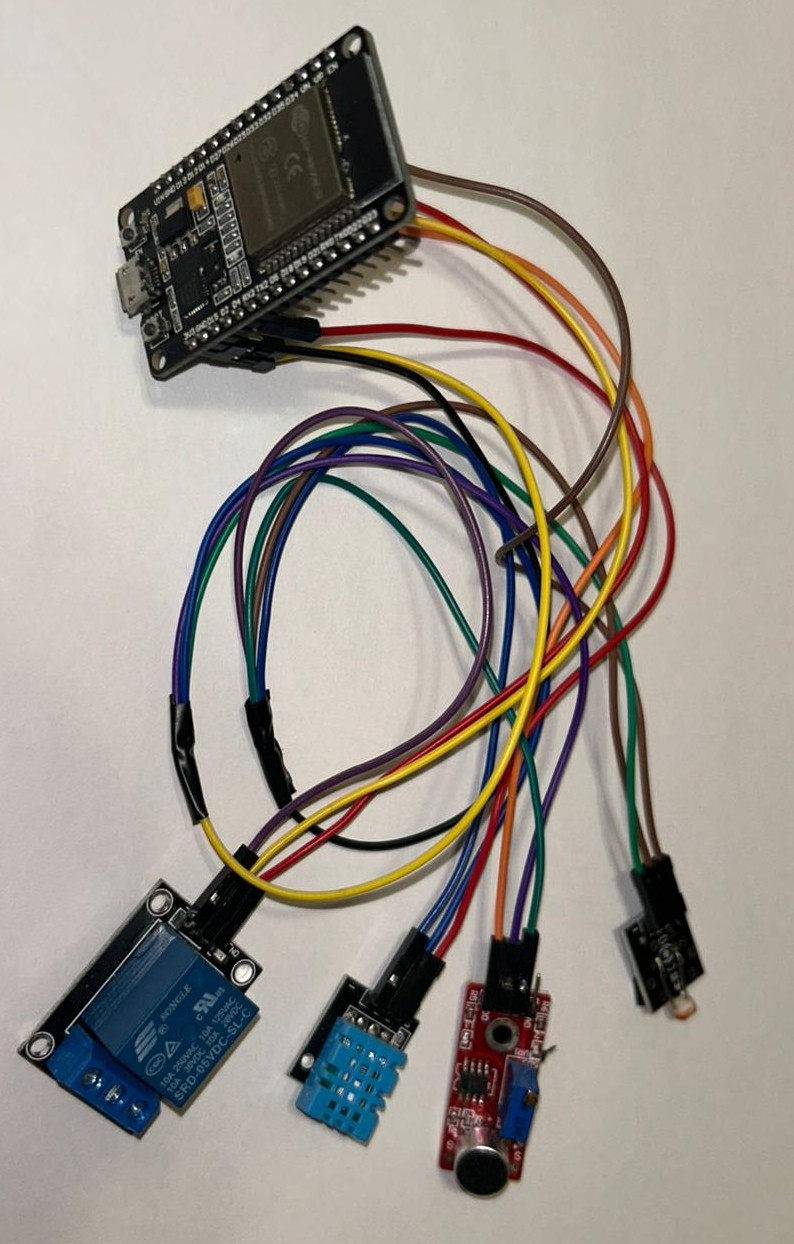
\includegraphics[width=\textwidth]{Img/nodo_ambiente.jpg}
        \caption{Módulo de Ambiente ($N_1$)}
        \label{fig:usr_nodo_amb}
    \end{subfigure}
    \hfill
    \begin{subfigure}[b]{0.32\textwidth}
        \centering
        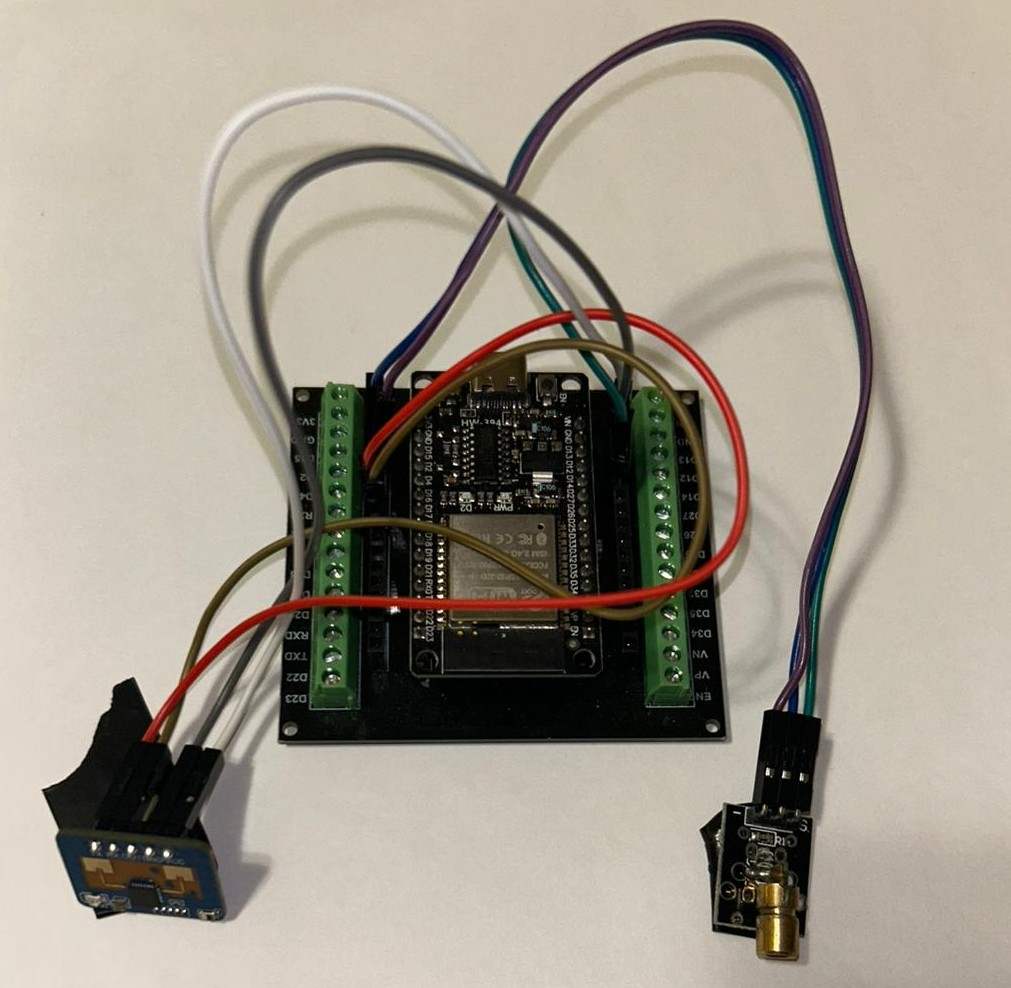
\includegraphics[width=\textwidth]{Img/nodo_escritorio.jpg}
        \caption{Módulo de Escritorio ($N_2$)}
        \label{fig:usr_nodo_esc}
    \end{subfigure}
    \hfill
    \begin{subfigure}[b]{0.32\textwidth}
        \centering
        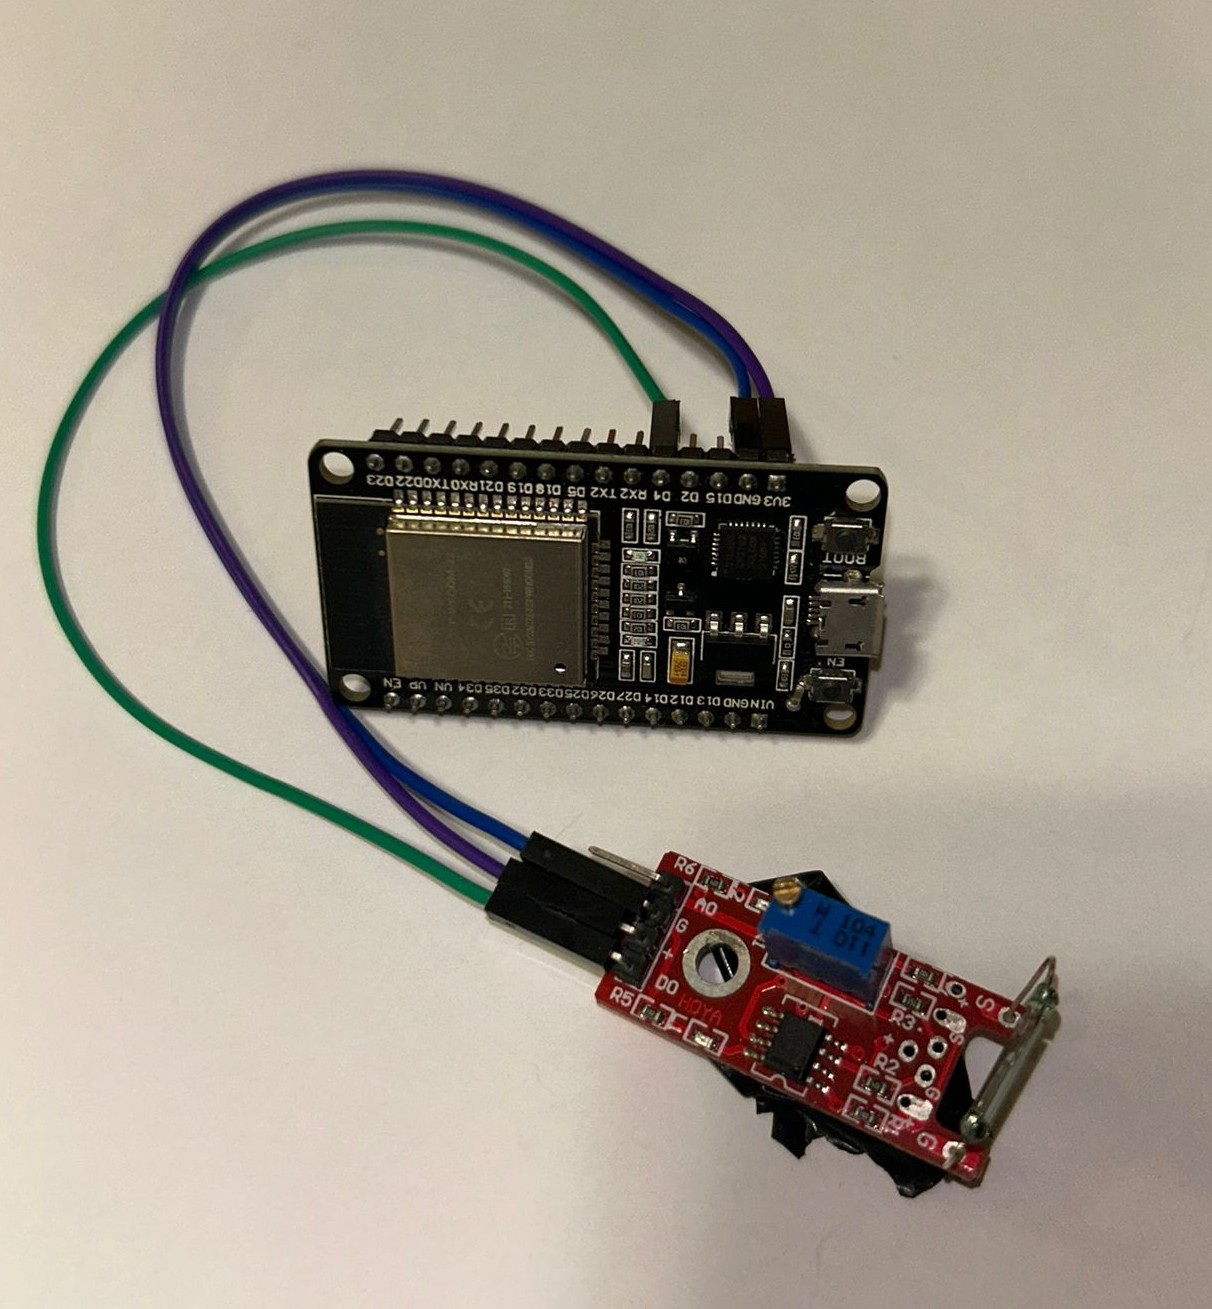
\includegraphics[width=\textwidth]{Img/nodo_puerta.jpg}
        \caption{Módulo de Puerta ($N_3$)}
        \label{fig:usr_nodo_puerta}
    \end{subfigure}
    \caption{Componentes de hardware y nodos sensores instalados en la habitación.}
    \label{fig:usr_nodos}
\end{figure}

\begin{enumerate}
    \item \textbf{Módulo de Ambiente ($N_1$):} mide la temperatura, la humedad y el nivel de ruido. Debe ubicarse en una zona de la pared libre de corrientes directas de aire acondicionado o calefactores. Incluye el interruptor electrónico que controla la corriente del enchufe general.
    \item \textbf{Módulo de Escritorio ($N_2$):} integra el sensor de presencia por radar y el fotorresistor de luminosidad. Debe colocarse sobre la mesa de trabajo, orientado diagonalmente hacia la silla del usuario a una distancia recomendada de entre 0.5 y 1.5 metros, asegurando que no haya objetos móviles interponiéndose (como aspas de ventiladores o cortinas).
    \item \textbf{Módulo de Puerta ($N_3$):} contiene el sensor magnético de contacto Reed. Se instala directamente sobre la hoja y el marco de la puerta de entrada para registrar los eventos físicos de apertura y cierre.
\end{enumerate}

Para que estos módulos se puedan comunicar con la red Wi-Fi y con el servidor central, es necesario programar los microcontroladores (las placas ESP32) por primera vez cargándoles su correspondiente software. Este proceso se gestiona de forma centralizada y visual desde la herramienta \textbf{ESPHome}, partiendo de la base de que ya disponemos de la Raspberry Pi en funcionamiento con Docker y los contenedores de \textbf{Home Assistant}, \textbf{ESPHome} y \textbf{Portainer} activos.

A continuación, se detalla el procedimiento que debe seguir el administrador o instalador para preparar y cargar el código en los módulos:
\begin{enumerate}
    \item \textbf{Acceder al panel de administración de ESPHome:} desde un ordenador conectado a la red local, abre el navegador de internet e introduce la dirección web del panel de ESPHome (habitualmente \texttt{http://ip\_raspberry\_pi:6052}, donde \texttt{ip\_raspberry\_pi} representa la dirección IP que proporciona Tailscale para tu Raspberry Pi). También puedes acceder a esta interfaz directamente desde la barra lateral izquierda de Home Assistant si está integrada.
    \item \textbf{Crear o seleccionar el dispositivo:} en la pantalla principal de ESPHome, haz clic en el botón ``+ Add Device'' para crear un nuevo dispositivo (o selecciona uno ya configurado de la lista). Dale un nombre descriptivo al módulo (ej. \texttt{nodo-ambiente}, \texttt{nodo-escritorio} o \texttt{nodo-puerta}).
    \item \textbf{Escribir la configuración de red y código:} introduce el código de configuración del módulo en formato de texto (los códigos específicos y completos para cada uno de los tres módulos se detallan más adelante en el Apéndice B, ``Manual Técnico y de Código''). Dentro del archivo de configuración, asegúrate de escribir correctamente los datos de tu red Wi-Fi:
    \begin{itemize}
        \item Nombre de la red Wi-Fi (\texttt{ssid}).
        \item Contraseña de la red Wi-Fi (\texttt{password}).
        \item Dirección IP fija asignada a ese módulo en concreto (para evitar conflictos de red y asegurar un acceso rápido).
    \end{itemize}
    \item \textbf{Conexión física y carga inicial del código:}
    Dado que es la primera vez que se programa la placa ESP32, la carga del software no puede hacerse de forma inalámbrica:
    \begin{enumerate}
        \item Conecta el módulo ESP32 físicamente mediante un cable micro-USB (o USB-C) a un puerto USB de tu ordenador, o bien directamente a uno de los puertos USB de la Raspberry Pi donde corre el sistema.
        \item En el panel de ESPHome, haz clic en el botón ``Install'' situado en la esquina superior derecha del dispositivo correspondiente.
        \item Si has conectado la placa a tu ordenador, selecciona la opción ``Plug into this computer'' (esta opción utiliza una tecnología del navegador Google Chrome o Edge para programarla directamente desde la web). Si has conectado la placa directamente a la Raspberry Pi, selecciona ``Plug into the server''.
        \item Haz clic en ``Install'' y espera a que el sistema compile el código y lo grabe en la placa (el proceso tardará un par de minutos y verás un registro de texto indicando el avance).
    \end{enumerate}
    \item \textbf{Instalación en ubicación definitiva y encendido:}
    Una vez programado con éxito el módulo por USB, ya puedes desconectarlo físicamente. A partir de este momento:
    \begin{enumerate}
        \item Coloca el módulo en su ubicación física recomendada en la estancia.
        \item Enchúfalo a una toma de corriente convencional utilizando cualquier cargador doméstico de móvil de $5\,\text{V}$ y un cable USB.
        \item Al recibir corriente, el microcontrolador iniciará de forma automática el software cargado, se conectará a la red Wi-Fi de tu casa y establecerá comunicación cifrada y segura con el servidor central para empezar a enviar lecturas.
    \end{enumerate}
    \item \textbf{Actualizaciones inalámbricas posteriores (OTA):} en el futuro, si necesitas hacer cualquier modificación en el comportamiento o los filtros del sensor, no tendrás que volver a conectar físicamente el módulo por USB. Podrás hacer las actualizaciones de forma inalámbrica por el aire seleccionando la opción ``Wirelessly'' dentro del menú ``Install'' de ESPHome.
\end{enumerate}

\subsection{Conexión y cableado de periféricos}
\label{sec:conexion_perifericos}

Para facilitar el ensamblado físico de los nodos sensores, se detallan a continuación los diagramas de cableado desarrollados con la herramienta de diseño electrónico \textbf{Fritzing}. En estos diagramas se representa de forma visual la placa de desarrollo ESP32, los sensores y actuadores asociados y la distribución de cables puente (Dupont) utilizando el código de colores estándar para alimentación ($5\,\text{V}$ en rojo, $3.3\,\text{V}$ en naranja, tierra o GND en negro) y líneas de datos (azul, amarillo o verde).

Al realizar las conexiones, es de vital importancia asegurar que los sensores compartan una masa común (GND) con el microcontrolador y que los niveles lógicos de entrada no superen la tolerancia máxima de $3.3\,\text{V}$ en los pines GPIO del ESP32.

\subsubsection{Cableado del Módulo de Ambiente (Nodo 1)}
El Módulo de Ambiente monitoriza variables higrométricas, iluminancia y nivel acústico de la estancia, además de controlar un relé optoacoplado. Las conexiones lógicas y de alimentación son las siguientes:
\begin{itemize}
    \item \textbf{Sensor DHT11 (Clima):} se alimenta a $3.3\,\text{V}$ (pin 3V3) y tierra (GND). Su pin de datos se conecta al \textbf{GPIO 4} del ESP32.
    \item \textbf{Fotorresistor LDR (Divisor de tensión):} se alimenta a $3.3\,\text{V}$ y GND. La salida analógica del divisor de tensión se conecta al canal ADC \textbf{GPIO 32} del ESP32.
    \item \textbf{Sensor de sonido KY-037 (Big Sound):} se alimenta a la línea de $5\,\text{V}$ (VIN) y GND para asegurar el correcto funcionamiento del comparador analógico. Su pin de salida digital (DO) se conecta al \textbf{GPIO 27} del ESP32.
    \item \textbf{Módulo de Relé (Control de enchufe):} se alimenta a $5\,\text{V}$ (VIN) y GND. Su pin de control (IN) se conecta al \textbf{GPIO 26} del ESP32.
\end{itemize}

En la Figura~\ref{fig:conexion_ambiente} se ilustra el conexionado completo del Nodo de Ambiente.

\begin{figure}[H]
    \centering
    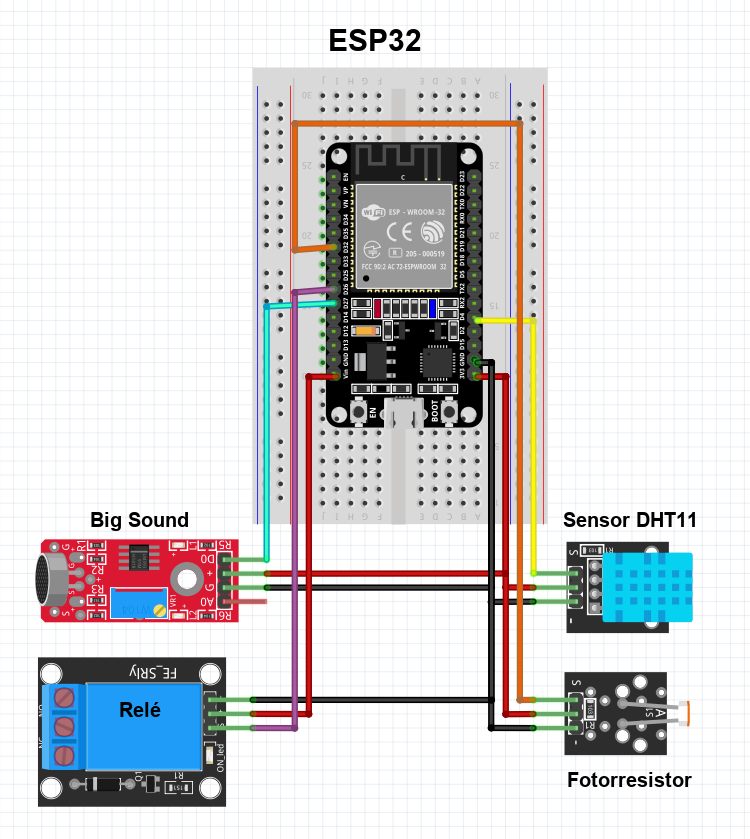
\includegraphics[width=0.65\textwidth]{Img/conexion_nodo_ambiente.png}
    \caption{Diagrama de conexionado de periféricos en Fritzing para el Módulo de Ambiente (Nodo 1).}
    \label{fig:conexion_ambiente}
\end{figure}

\subsubsection{Cableado del Módulo de Escritorio (Nodo 2)}
El Módulo de Escritorio integra el radar de microondas FMCW y el emisor láser. Su cableado se organiza de la siguiente manera:
\begin{itemize}
    \item \textbf{Radar mmWave HLK-LD2410C:} requiere una tensión de alimentación estable de $5\,\text{V}$ (VIN) y GND. La transmisión de datos se realiza a través de un canal serie UART cruzado: el pin de transmisión (TX) del radar se conecta al pin de recepción del ESP32 \textbf{RX2 (GPIO 16)}, y el pin de recepción (RX) del radar se conecta al pin de transmisión del ESP32 \textbf{TX2 (GPIO 17)}.
    \item \textbf{Módulo Emisor Láser KY-008:} se conecta directamente a la línea lógica \textbf{GPIO 12} del ESP32 para el control de encendido y apagado digital, y su pin de tierra a GND.
\end{itemize}

En la Figura~\ref{fig:conexion_escritorio} se muestra el conexionado correspondiente al Nodo de Escritorio.

\begin{figure}[H]
    \centering
    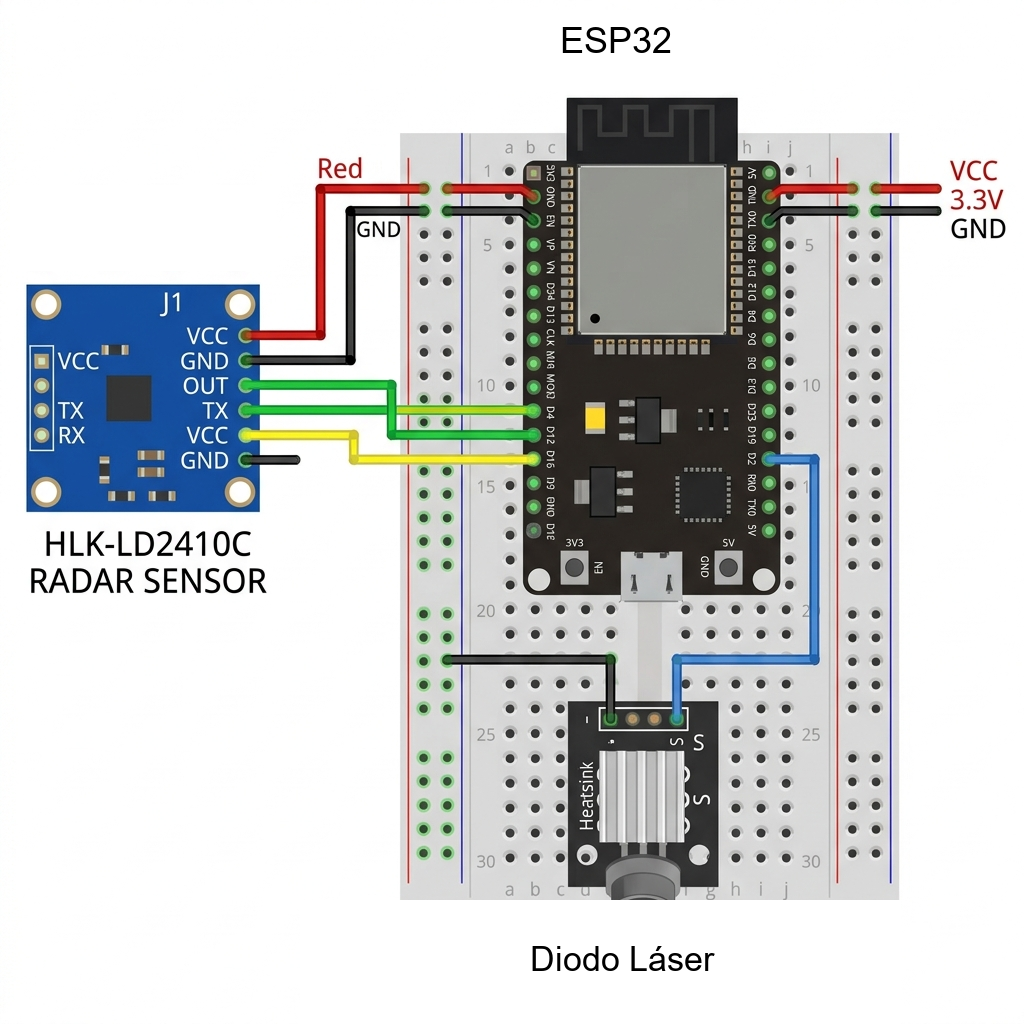
\includegraphics[width=0.65\textwidth]{Img/conexion_nodo_escritorio.png}
    \caption{Diagrama de conexionado de periféricos en Fritzing para el Módulo de Escritorio (Nodo 2).}
    \label{fig:conexion_escritorio}
\end{figure}

\subsubsection{Cableado del Módulo de Puerta (Nodo 3)}
El Módulo de Puerta monitoriza exclusivamente el acceso magnético de la puerta de entrada. Sus conexiones físicas son sumamente sencillas:
\begin{itemize}
    \item \textbf{Sensor Reed Switch (Contacto magnético):} se conecta directamente entre el pin \textbf{GPIO 4} del ESP32 y el pin de tierra (GND). Para simplificar el hardware y evitar el uso de resistencias físicas externas de acoplamiento, se aprovecha la resistencia de pull-up interna del microcontrolador, la cual se activa y configura mediante software.
\end{itemize}

En la Figura~\ref{fig:conexion_puerta} se ilustra el conexionado completo para el Módulo de Puerta.

\begin{figure}[H]
    \centering
    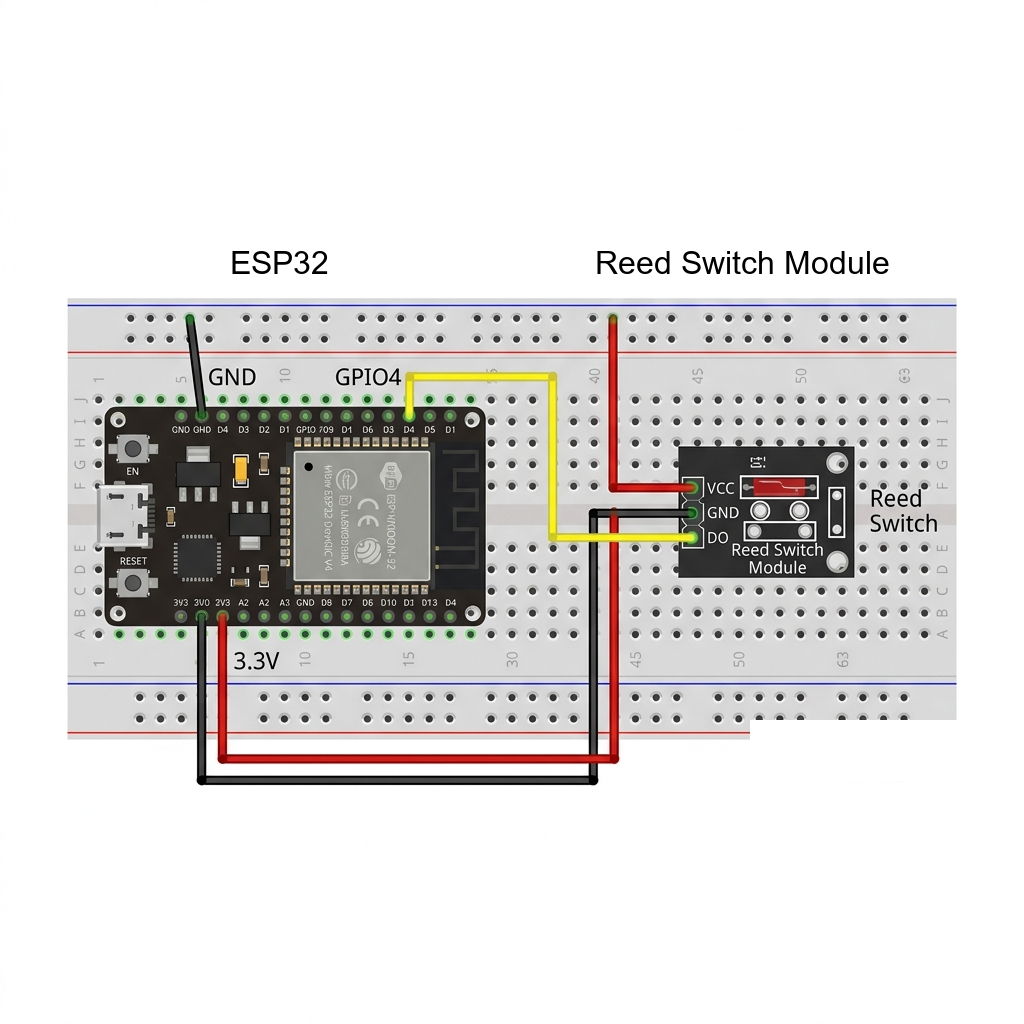
\includegraphics[width=0.65\textwidth]{Img/conexion_nodo_puerta.png}
    \caption{Diagrama de conexionado de periféricos en Fritzing para el Módulo de Puerta (Nodo 3).}
    \label{fig:conexion_puerta}
\end{figure}

\subsection{Manual de acceso y conexión}
Para ver el estado de la habitación y controlar las luces, puedes utilizar un ordenador, una tablet o tu teléfono móvil. Existen dos formas de conectarse dependiendo de dónde te encuentres:

\subsubsection{Acceso desde casa (Red Wi-Fi local)}
Si estás conectado a la misma red Wi-Fi de tu casa, el acceso es directo:
\begin{enumerate}
    \item Abre el navegador de internet que utilices habitualmente (Google Chrome, Safari, etc.) en tu ordenador o móvil.
    \item Introduce la dirección web que se te ha proporcionado para el sistema (habitualmente \texttt{http://192.168.1.150:8123}).
    \item Introduce tu nombre de usuario y tu contraseña.
\end{enumerate}

\subsubsection{Acceso desde fuera de casa (Conexión remota segura)}
Si estás en la calle, en el trabajo o de viaje, puedes seguir accediendo a tu sistema gracias a una red privada segura que conecta tu móvil directamente con tu casa:
\begin{enumerate}
    \item Instala la aplicación gratuita llamada \textbf{Tailscale} en tu teléfono móvil o en tu ordenador portátil (disponible en la tienda de aplicaciones de Android y Apple).
    \item Abre la aplicación Tailscale e inicia sesión con la cuenta de usuario que te haya configurado el administrador del sistema.
    \item Activa la conexión en la aplicación (deslizando el interruptor de encendido).
    \item Abre tu navegador de internet e introduce la misma dirección web que usas en casa. ¡Ya estarás conectado de forma segura!
\end{enumerate}

\subsection{Manual del panel de control (interfaz Lovelace)}
Una vez accedas, verás una pantalla organizada en tarjetas visuales muy intuitivas, diseñada para mostrarte toda la información de un solo vistazo (véase la Figura~\ref{fig:usr_dashboard1}):

\begin{figure}[H]
    \centering
    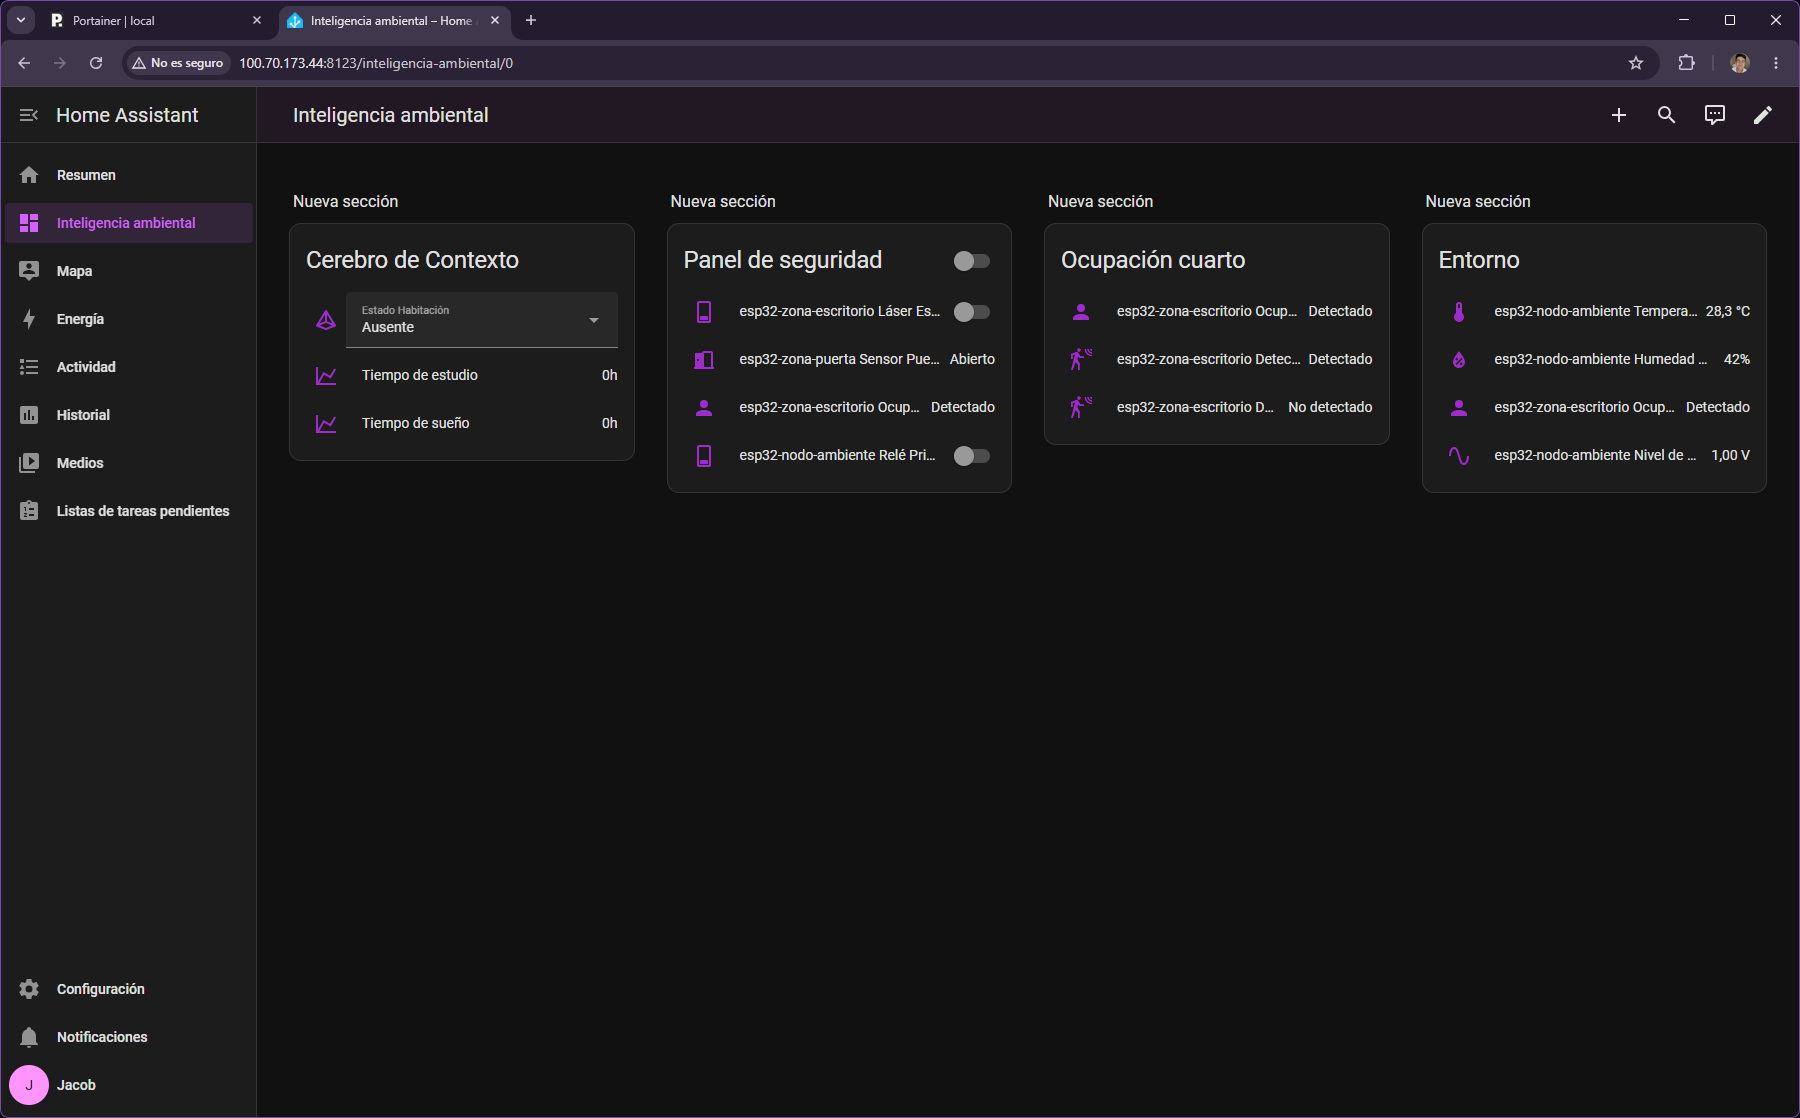
\includegraphics[width=0.90\textwidth]{Img/ha_dashboard_lovelace1.png}
    \caption{Pantalla principal del panel de control (Cuadro de Mandos Lovelace) en Home Assistant.}
    \label{fig:usr_dashboard1}
\end{figure}

\begin{itemize}
    \item \textbf{Interruptores de Control Manual:} en la parte superior verás botones para encender o apagar manualmente la luz de estudio del escritorio en cualquier momento, además de activar o desactivar la alarma del sistema.
    \item \textbf{Estado de Presencia:} la tarjeta central te muestra si hay alguien detectado en el escritorio o en la habitación en general. Gracias al radar de alta precisión, la pantalla te indicará si estás ``Sentado en Escritorio'', ``Descansando'' o si la habitación está ``Ausente''.
    \item \textbf{Mediciones del Entorno:} podrás ver de forma clara e instantánea la temperatura actual, el nivel de humedad y el nivel de ruido en la estancia.
    \item \textbf{Seguridad de Accesos:} indica si la puerta de la estancia está ``Abierta'' o ``Cerrada'', así como el estado del haz de luz de la barrera láser de la puerta.
    \item \textbf{Históricos y Gráficas de Actividad:} deslizando hacia la parte inferior del panel (o accediendo a la sección de históricos, Figura~\ref{fig:usr_dashboard2}), puedes revisar gráficas visuales que muestran cómo ha cambiado la temperatura a lo largo de las últimas horas, cuándo se abrió la puerta o a qué horas estuviste utilizando el escritorio.
\end{itemize}

\begin{figure}[H]
    \centering
    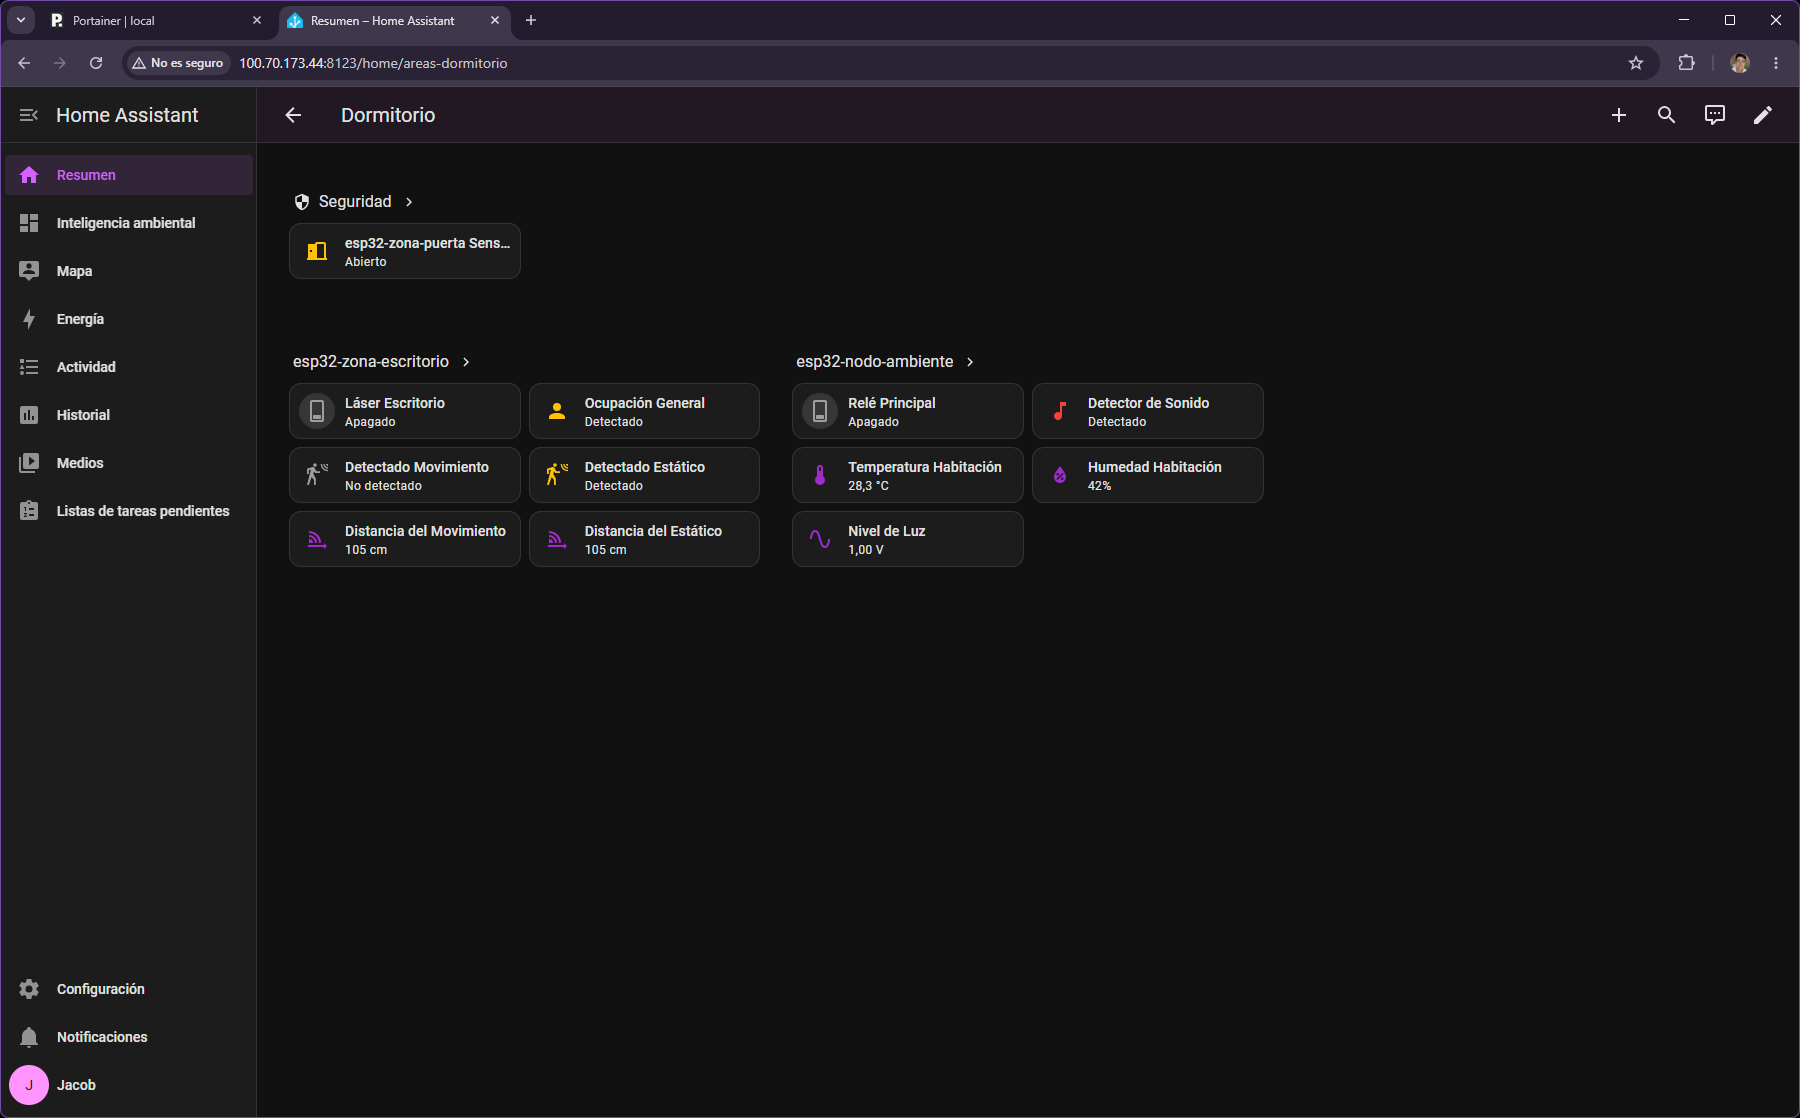
\includegraphics[width=0.90\textwidth]{Img/ha_dashboard_lovelace2.png}
    \caption{Sección de históricos y registros del panel de control.}
    \label{fig:usr_dashboard2}
\end{figure}

\subsection{Manual del comportamiento inteligente (automatizaciones)}
Para que no tengas que preocuparte de encender o apagar interruptores constantemente, el sistema ha sido programado con comportamientos automáticos inteligentes. A continuación te explicamos cómo funcionan:

\begin{enumerate}
    \item \textbf{Control automático de la luz del escritorio:}
    Cuando entres a la estancia y te sientes en la silla del escritorio, el sistema lo detectará al instante. Si es de noche o hay poca luz natural en la habitación, la luz del escritorio se encenderá automáticamente para que trabajes con comodidad. Al levantarte e irte del escritorio, la luz se apagará sola transcurridos unos instantes para ahorrar energía.
    
    \item \textbf{Avisos de descanso saludables (Método Pomodoro):}
    Pasar muchas horas seguidas sentado es perjudicial para la salud. Por ello, si el sistema de radar detecta que llevas más de 25 minutos seguidos sentado en el escritorio, la luz del escritorio realizará un parpadeo en color naranja y recibirás un mensaje de aviso en tu teléfono móvil indicándote que es hora de levantarte, beber agua y estirar las piernas durante un breve descanso de 5 minutos.
    
    \item \textbf{Sistema de alarma de la habitación:}
    Cuando vayas a salir de casa, puedes activar el ``Modo Alarma'' desde el panel de control en tu móvil. Si alguien abre la puerta de la habitación o cruza el haz de luz láser mientras la alarma está activa, el sistema lo considerará una intrusión: la luz de la habitación parpadeará en color rojo para alertar visualmente y recibirás una notificación de emergencia inmediata en tu teléfono móvil con el aviso.
    
    \item \textbf{Ahorro de energía automático (Modo Noche y Ausencia):}
    Si sales de la habitación y el sistema no detecta ningún movimiento ni respiración durante 10 minutos, apagará de forma automática todas las luces y aparatos eléctricos. De igual forma, si te vas a dormir y activas el ``Modo Noche'', el sistema apagará instantáneamente todos los equipos para asegurar tu descanso y evitar consumos innecesarios.
\end{enumerate}

\subsection{Guía de resolución de incidencias}
Esta sección recopila los problemas más comunes divididos en función del perfil de uso, facilitando tanto el diagnóstico rápido por parte del usuario final como la resolución de fallos lógicos o físicos de despliegue por parte del instalador.

\subsubsection{Incidencias de uso cotidiano (usuario final)}
A continuación, se describen los problemas relacionados con la operación y uso ordinario del sistema:

\begin{itemize}
    \item \textbf{La luz del escritorio no se enciende sola cuando me siento:}
    \begin{enumerate}
        \item Comprueba si hay suficiente luz natural en la habitación. Recuerda que el sistema está configurado para no encender la luz si la estancia ya está suficientemente iluminada por el sol.
        \item Asegúrate de que la lámpara esté enchufada al módulo de corriente y que el interruptor físico propio de la lámpara esté en posición de encendido.
    \end{enumerate}
    
    \item \textbf{En la pantalla aparece que un sensor no está disponible:}
    \begin{enumerate}
        \item Verifica que el módulo sensor en cuestión ($N_1$, $N_2$ o $N_3$) esté conectado a su cargador y que el cargador esté bien enchufado a la toma de corriente.
        \item Si el módulo está encendido, es posible que haya habido un corte temporal en la conexión Wi-Fi de tu casa. El dispositivo volverá a conectarse solo automáticamente una vez la red Wi-Fi se estabilice.
    \end{enumerate}
    
    \item \textbf{No puedo acceder al panel de control desde fuera de casa:}
    \begin{enumerate}
        \item Asegúrate de tener conexión a internet en tu móvil (datos móviles o Wi-Fi externo).
        \item Comprueba que tienes la aplicación \textbf{Tailscale} abierta y que el interruptor principal de conexión dentro de la aplicación esté activo.
    \end{enumerate}
\end{itemize}

\subsubsection{Incidencias de instalación y configuración (administrador/instalador)}
Esta sección aborda problemas específicos que pueden surgir durante el montaje de hardware, la programación de las placas o el despliegue del servidor central:

\begin{itemize}
    \item \textbf{El microcontrolador ESP32 no es reconocido por el ordenador al conectarlo por USB:}
    \begin{enumerate}
        \item \textbf{Causa:} Falta del controlador del puente USB-a-UART en el sistema operativo del ordenador. Las placas de desarrollo ESP32 comerciales suelen integrar chips conversores como el CP2102 de Silicon Labs o el CH340 de WCH.
        \item \textbf{Solución:} Descarga e instala los controladores oficiales del fabricante del chip (Silicon Labs CP210x USB to UART Bridge VCP Drivers o WCH CH340 Driver) correspondientes al sistema operativo utilizado (Windows, macOS o Linux).
        \item \textbf{Verificación:} Conecta de nuevo el microcontrolador y verifica que se asigne un puerto COM (en Windows) o un dispositivo de terminal virtual (en macOS/Linux, como \texttt{/dev/ttyUSB0}).
    \end{enumerate}

    \item \textbf{La Raspberry Pi 4 se queda colgada o se reinicia durante la compilación del código en ESPHome:}
    \begin{enumerate}
        \item \textbf{Causa:} Sobrecarga extrema de CPU y memoria RAM. El compilador de C++ integrado en ESPHome consume una gran cantidad de recursos, lo que puede agotar la memoria de la Raspberry Pi (especialmente en modelos de 1\,GB o 2\,GB de RAM o bajo configuraciones sin memoria de intercambio (\textit{swap})).
        \item \textbf{Solución A (Compilación local en PC):} Abre ESPHome, selecciona el menú de tres puntos del nodo y haz clic en ``Manual Download'' para compilar el firmware utilizando los recursos del ordenador local. Una vez descargado el archivo ejecutable compilado (\texttt{.bin}), utiliza el cargador web oficial de ESPHome (\texttt{https://web.esphome.io}) o la herramienta gráfica ESPHome Flasher desde el ordenador para grabar el código directamente en la placa ESP32 por USB.
        \item \textbf{Solución B (Optimización en la Raspberry Pi):} Configura un archivo de intercambio (\textit{swapfile}) de al menos 1\,GB en Raspberry Pi OS para dar soporte a la memoria RAM física en tareas de compilación intensa.
    \end{enumerate}

    \item \textbf{Inestabilidad general en la Raspberry Pi, apagados aleatorios o falta de detección de periféricos USB:}
    \begin{enumerate}
        \item \textbf{Causa:} Alimentación eléctrica deficiente. La Raspberry Pi 4 requiere una fuente de alimentación estable de $5\,\text{V}$ y un mínimo de $3\,\text{A}$ ($15\,\text{W}$). El uso de cargadores de móvil genéricos, cables USB de mala calidad o puertos USB de ordenador suele provocar caídas de tensión. Esto impide el correcto funcionamiento de componentes internos o de dispositivos conectados (como discos externos o módulos USB).
        \item \textbf{Solución:} Sustituye la fuente de alimentación por el adaptador oficial de corriente de la Raspberry Pi 4 o un cargador certificado compatible que garantice una salida dedicada de $5.1\,\text{V}$ y $3.0\,\text{A}$.
    \end{enumerate}

    \item \textbf{Los nodos ESP32 no logran conectarse a la red inalámbrica Wi-Fi:}
    \begin{enumerate}
        \item \textbf{Causa:} Incompatibilidad de banda de frecuencia de red. Los microcontroladores basados en el SoC ESP32 solo son compatibles con la banda de $2.4\,\text{GHz}$. Si el enrutador de acceso doméstico trabaja únicamente en la banda de $5\,\text{GHz}$ o tiene activo un sistema híbrido de autogestión de banda (Smart Connect) que obliga al nodo a enlazarse en $5\,\text{GHz}$, la conexión fallará.
        \item \textbf{Solución:} Accede al panel de configuración del enrutador y asegúrate de que la banda de $2.4\,\text{GHz}$ esté habilitada con un canal específico. Si el sistema híbrido da problemas, es recomendable configurar una red Wi-Fi virtual (SSID secundario) dedicada en exclusiva a dispositivos IoT forzada a operar en $2.4\,\text{GHz}$.
    \end{enumerate}

    \item \textbf{Las entidades de los nodos sensores aparecen en Home Assistant como ``No disponibles'':}
    \begin{enumerate}
        \item \textbf{Causa:} Desajuste en la clave de cifrado de la API o problemas de enrutamiento de red local.
        \item \textbf{Solución:} Abre el archivo de configuración del nodo en el panel de ESPHome y comprueba la clave de la API en la sección \texttt{api: encryption: key}. Verifica que esta clave de seguridad sea idéntica a la que introdujiste en la integración de Home Assistant. Si la clave es correcta, asegúrate de que la Raspberry Pi y las placas ESP32 se encuentren en la misma subred de red local y que los puertos de comunicación (por defecto, puerto TCP \texttt{6053}) no estén bloqueados por políticas de aislamiento de red del router.
    \end{enumerate}
\end{itemize}

\newpage
\section{Manual técnico y de código}
\label{anexo:manual_tecnico_codigo}

En este anexo se detalla el conjunto completo de códigos y configuraciones desarrollados para el despliegue del sistema domótico local. Se incluye la infraestructura de red virtualizada bajo Docker, el código declarativo de firmware para los tres nodos inalámbricos basados en ESPHome y las nueve automatizaciones que gobiernan la lógica de contexto y bienestar en el servidor central Home Assistant.

\subsection{Infraestructura y contenedores perimetrales (Docker)}
El servidor central se implementa sobre una placa Raspberry Pi 4 ejecutando el sistema operativo Raspberry Pi OS. Para garantizar el aislamiento de dependencias, la portabilidad y la reproducibilidad técnica, los servicios de Home Assistant, ESPHome y Portainer se orquestan como contenedores independientes compartiendo el espacio de red física del host.

A continuación, se presenta la especificación del archivo de gestión centralizada \texttt{docker-compose.yml}:

\begin{lstlisting}[language=YAML, caption={Archivo de gestión centralizada de contenedores en la Raspberry Pi 4 (docker-compose.yml).}, label={lst:docker_compose}]
version: '3.8'

services:
  homeassistant:
    container_name: homeassistant
    image: 'ghcr.io/home-assistant/home-assistant:stable'
    volumes:
      - /home/jpmorenito/homeassistant/config:/config
      - /etc/localtime:/etc/localtime:ro
    environment:
      - TZ=Europe/Madrid
    restart: unless-stopped
    privileged: true
    network_mode: host

  esphome:
    container_name: esphome
    image: 'ghcr.io/esphome/esphome:latest'
    volumes:
      - /home/jpmorenito/esphome/config:/config
      - /etc/localtime:/etc/localtime:ro
    environment:
      - TZ=Europe/Madrid
    restart: unless-stopped
    privileged: true
    network_mode: host

  portainer:
    container_name: portainer
    image: 'portainer/portainer-ce:latest'
    command: -H unix:///var/run/docker.sock
    ports:
      - '9000:9000'
    volumes:
      - /var/run/docker.sock:/var/run/docker.sock
      - portainer_data:/data
      - /etc/localtime:/etc/localtime:ro
    restart: unless-stopped

volumes:
  portainer_data:
\end{lstlisting}

\subsection{Firmware de los nodos perimetrales (ESPHome)}
Los nodos perimetrales inalámbricos se basan en el microcontrolador SoC ESP32. Su programación se realiza mediante archivos de configuración declarativos en formato YAML, que el compilador de ESPHome traduce automáticamente a código de producción C++ optimizado.

\subsubsection{Nodo de ambiente (esp32-nodo-ambiente.yaml)}
Este firmware gestiona la lectura unifilar del sensor de temperatura y humedad DHT11, la entrada analógica del fotorresistor LDR, el detector acústico digital filtrado contra rebotes electromecánicos y el relé de estado sólido que controla la iluminación principal de la estancia.

\begin{lstlisting}[language=YAML, caption={Firmware completo del Nodo de Ambiente.}, label={lst:code_nodo_ambiente}]
esphome:
  name: esp32-nodo-ambiente
  friendly_name: esp32-nodo-ambiente

esp32:
  board: esp32dev
  framework:
    type: arduino

logger:

wifi:
  ssid: 'Livebox6s-479B'
  password: 'jjCLnhaS56aA'

api:

ota:
  - platform: esphome

# 1. SENSOR DE TEMPERATURA Y HUMEDAD
sensor:
  - platform: dht
    pin: 4
    # ATENCION: Si tu sensor es el azul pon DHT11, si es el blanco pon DHT22.
    model: DHT11 
    temperature:
      name: 'Temperatura Habitacion'
    humidity:
      name: 'Humedad Habitacion'
    update_interval: 30s

# 2. SENSOR DE LUMINOSIDAD (FOTORESISTOR LDR)
  - platform: adc
    pin: 32
    name: 'Nivel de Luz'
    update_interval: 10s
    attenuation: auto

# 3. ACTUADOR: RELE
switch:
  - platform: gpio
    pin: 26
    name: 'Rele Principal'
    id: rele_1
    restore_mode: ALWAYS_OFF

# 4. SENSOR DE RUIDO (BIG SOUND)
binary_sensor:
  - platform: gpio
    pin: 27
    name: 'Detector de Sonido'
    device_class: sound
    filters:
      # Pequeno filtro para que no mande 50 avisos por segundo al dar una palmada
      - delayed_off: 500ms
\end{lstlisting}

\subsubsection{Nodo de escritorio (esp32-zona-escritorio.yaml)}
Este firmware inicializa el bus de comunicación serie UART a 256.000 baudios para procesar la telemetría espacial del radar de microondas FMCW (HLK-LD2410). Expone tanto los estados binarios de detección como las métricas analógicas de distancia, además de incorporar el interruptor digital para el emisor láser secundario.

\begin{lstlisting}[language=YAML, caption={Firmware completo del Nodo de Escritorio.}, label={lst:code_nodo_escritorio}]
esphome:
  name: esp32-zona-escritorio
  friendly_name: esp32-zona-escritorio

esp32:
  board: esp32dev
  framework:
    type: arduino

logger:

wifi:
  ssid: 'Livebox6s-479B'
  password: 'jjCLnhaS56aA'

api:

ota:
  - platform: esphome

# CONFIGURACION DEL RADAR LD2410
uart:
  tx_pin: 17
  rx_pin: 16
  baud_rate: 256000
  parity: NONE
  stop_bits: 1

ld2410:

# 1. SENSORES BINARIOS DEL RADAR
binary_sensor:
  - platform: ld2410
    has_target:
      name: 'Ocupacion General'
    has_moving_target:
      name: 'Detectado Movimiento'
    has_still_target:
      name: 'Detectado Estatico'

# 2. SENSORES DE DISTANCIA DEL RADAR
sensor:
  - platform: ld2410
    moving_distance:
      name: 'Distancia del Movimiento'
    still_distance:
      name: 'Distancia del Estatico'

# 3. CONTROLES DESLIZANTES DEL RADAR
number:
  - platform: ld2410
    timeout:
      name: 'Tiempo de retardo (Timeout)'
    max_move_distance_gate:
      name: 'Limite distancia Movimiento'
    max_still_distance_gate:
      name: 'Limite distancia Estatico'

# 4. ACTUADOR: EMISOR LASER
switch:
  - platform: gpio
    pin: 12 
    name: 'Laser Escritorio'
    id: laser_escritorio
    restore_mode: ALWAYS_OFF
\end{lstlisting}

\subsubsection{Nodo de puerta (esp32-zona-puerta.yaml)}
Este firmware controla la monitorización digital del sensor de contacto magnético (interruptor Reed) en la puerta de acceso, aplicando filtros antirebote de 100\,ms por software para registrar los eventos de apertura y cierre de forma inmediata.

\begin{lstlisting}[language=YAML, caption={Firmware completo del Nodo de Puerta.}, label={lst:code_nodo_puerta}]
esphome:
  name: esp32-zona-puerta
  friendly_name: esp32-zona-puerta

esp32:
  board: esp32dev
  framework:
    type: arduino

logger:

wifi:
  ssid: 'Livebox6s-479B'
  password: 'jjCLnhaS56aA'

api:

ota:
  - platform: esphome

# 1. SENSOR DE PUERTA MAGNETICO
binary_sensor:
  - platform: gpio
    pin:
      number: 4
      mode:
        input: true
        pullup: true
    name: 'Sensor Puerta'
    device_class: door
    filters:
      - delayed_on: 100ms
      - delayed_off: 100ms
\end{lstlisting}

\subsection{Automatizaciones del servidor central perimetral (Home Assistant)}
El archivo de configuración \texttt{automations.yaml} aloja el motor de reglas lógicas que rigen el comportamiento inteligente de la estancia. Se detallan a continuación las nueve automatizaciones operativas:

\subsubsection{Termostato inteligente (modo estudio)}
Activa de forma automatizada un actuador auxiliar de potencia (cuyo proxy Bluetooth comanda el encendido eléctrico de un radiador local) si el estado de contexto determinado para la estancia es de \texttt{Estudio} ininterrumpido durante 5 minutos y la lectura térmica desciende por debajo de 19,5\,\text{°C}.

\begin{lstlisting}[language=YAML, caption={Código de control térmico reactivo al contexto de estudio.}, label={lst:auto_climatizacion}]
- id: 'climatizacion_estudio_001'
  alias: 'Termostato Inteligente: Modo Estudio'
  trigger:
    - platform: 'state'
      entity_id: 'sensor.contexto_de_la_habitacion'
      to: 'Actividad / Estudiando'
      for:
        minutes: 5
  condition:
    - condition: 'numeric_state'
      entity_id: 'sensor.esp32_nodo_ambiente_temperatura_habitacion'
      below: 19.5
  action:
    - service: 'switch.turn_on'
      target:
        entity_id: 'switch.bluetooth_proxy_ea49ac_actuador_dormitorio'
\end{lstlisting}

\subsubsection{Resumen diario de bienestar (calidad de vida)}
Regla de análisis local ejecutada diariamente a las 22:00:00. Evalúa los históricos de tiempo activo en el escritorio y las horas de descanso nocturno y genera un reporte analítico adaptativo mediante plantillas Jinja2, el cual es transmitido por vía de notificación push al usuario sin contactar con servidores externos.

\begin{lstlisting}[language=YAML, caption={Código del analista de bienestar diario local.}, label={lst:auto_bienestar_resumen}]
- id: 'informe_diario_qol'
  alias: 'Analista Local: Resumen Diario de Bienestar'
  description: 'Genera un reporte diario analizando las horas de estudio y sueno del nuevo motor de contexto.'
  triggers:
    - at: '22:00:00'
      trigger: 'time'
  actions:
    - data:
        title: 'Informe de Inteligencia Ambiental'
        message: |
          Resumen de tu jornada: - Tiempo efectivo de estudio: {{ states(''sensor.tiempo_de_estudio'') }} horas. - Tiempo de descanso (anoche): {{ states(''sensor.tiempo_de_sueno'') }} horas.
          {% if states(''sensor.tiempo_de_estudio'') | float > 4.0 %}
            Gran rendimiento hoy. El sistema ha mantenido un confort termico constante.
          {% else %}
            Jornada ligera. Sistemas en modo ahorro energetico.
          {% endif %}
      action: 'notify.notify'
  mode: 'single'
\end{lstlisting}

\subsubsection{Detección espacial de la zona de estudio (radar)}
Esta regla infiere el paso de la estancia a modo de \texttt{Estudio} basándose en la distancia reportada por la telemetría del radar LD2410 del Nodo de Escritorio. Si el radar reporta la presencia estática de un cuerpo en un radio inferior a 1,2 metros durante más de 2 minutos, se conmuta el estado lógico general de la estancia a \texttt{Estudio}. Por contra, si no se registra presencia en ese radio durante el mismo lapso, el sistema devuelve el contexto a \texttt{Ocio}.

\begin{lstlisting}[language=YAML, caption={Fusión de distancia de radar para la detección de la zona de estudio.}, label={lst:auto_detect_estudio}]
- id: '1779303721704'
  alias: 'Contexto: Deteccion de Estudio (Radar Espacial)'
  description: 'Infiere si estas estudiando basandose en tu distancia al radar LD2410.'
  triggers:
    - entity_id: 'sensor.esp32_zona_escritorio_distancia_del_estatico'
      below: 120
      for:
        minutes: 2
      id: 'en_escritorio'
      trigger: 'numeric_state'
    - entity_id: 'sensor.esp32_zona_escritorio_distancia_del_estatico'
      above: 120
      for:
        minutes: 2
      id: 'fuera_de_escritorio'
      trigger: 'numeric_state'
  conditions:
    - condition: 'state'
      entity_id: 'input_select.estado_habitacion'
      state:
        - 'Ocio'
        - 'Estudio'
  actions:
    - choose:
        - conditions:
            - condition: 'trigger'
              id: 'en_escritorio'
          sequence:
            - target:
                entity_id: 'input_select.estado_habitacion'
              data:
                option: 'Estudio'
              action: 'input_select.select_option'
        - conditions:
            - condition: 'trigger'
              id: 'fuera_de_escritorio'
          sequence:
            - target:
                entity_id: 'input_select.estado_habitacion'
              data:
                option: 'Ocio'
              action: 'input_select.select_option'
  mode: 'single'
\end{lstlisting}

\subsubsection{Fusión sensorial para la detección del sueño (radar y LDR)}
Infiere dinámicamente si el usuario se encuentra durmiendo o si se ha despertado. Transiciona al estado \texttt{Durmiendo} si el sensor LDR del Nodo Ambiente registra un valor de luminosidad inferior a 0,5\,V de forma ininterrumpida durante 10 minutos. Para transicionar de vuelta al modo de vigilia (\texttt{Ocio}), el motor lógico requiere que el radar del Nodo Escritorio registre movimiento continuo durante al menos 2 minutos, o bien que la luminosidad analógica en la estancia supere el umbral de 1\,V durante el mismo intervalo.

\begin{lstlisting}[language=YAML, caption={Regla lógica de transiciones de sueño mediante fusión de luminosidad y radar.}, label={lst:auto_detect_sueno}]
- id: '1779306431260'
  alias: 'Contexto: Deteccion de Sueno (Fusion Radar + LDR)'
  description: 'Infiere si estas durmiendo o si te has despertado cruzando la luz y el movimiento.'
  triggers:
    - entity_id: 'sensor.esp32_nodo_ambiente_nivel_de_luz'
      below: 0.5
      for:
        minutes: 10
      id: 'se_duerme'
      trigger: 'numeric_state'
    - entity_id: 'binary_sensor.esp32_zona_escritorio_detectado_movimiento'
      to: 'on'
      for:
        minutes: 2
      id: 'se_despierta_movimiento'
      trigger: 'state'
    - entity_id: 'sensor.esp32_nodo_ambiente_nivel_de_luz'
      above: 1
      for:
        minutes: 2
      id: 'se_despierta_luz'
      trigger: 'numeric_state'
  conditions: []
  actions:
    - choose:
        - conditions:
            - condition: 'trigger'
              id: 'se_duerme'
            - condition: 'state'
              entity_id: 'input_select.estado_habitacion'
              state: 'Ocio'
          sequence:
            - target:
                entity_id: 'input_select.estado_habitacion'
              data:
                option: 'Durmiendo'
              action: 'input_select.select_option'
        - conditions:
            - condition: 'or'
              conditions:
                - condition: 'trigger'
                  id: 'se_despierta_movimiento'
                - condition: 'trigger'
                  id: 'se_despierta_luz'
            - condition: 'state'
              entity_id: 'input_select.estado_habitacion'
              state: 'Durmiendo'
          sequence:
            - target:
                entity_id: 'input_select.estado_habitacion'
              data:
                option: 'Ocio'
              action: 'input_select.select_option'
  mode: 'single'
\end{lstlisting}

\subsubsection{Alarma de intrusión de seguridad perimetral}
Gobierna la seguridad perimetral de la estancia cuando se activa de forma manual (representado por el encendido físico del emisor láser del escritorio). Si se detecta presencia física mediante el radar de ondas milimétricas en el Nodo Escritorio (\texttt{binary\_sensor.esp32\_zona\_escritorio\_ocupacion\_general} en estado encendido) mientras el láser está activo, el sistema dispara de forma inmediata una alarma: envía una alerta de intrusión push de prioridad crítica y fuerza el encendido eléctrico de la luminaria principal a través del relé físico para disuadir al intruso.

\begin{lstlisting}[language=YAML, caption={Automatización de alarma perimetral reactiva al radar.}, label={lst:auto_seguridad_alarma}]
- id: '1779308813969'
  alias: 'Seguridad: Alarma por Radar (Modo Manual)'
  description: 'Dispara la alarma si el radar detecta presencia mientras el laser esta encendido.'
  triggers:
    - entity_id: 'binary_sensor.esp32_zona_escritorio_ocupacion_general'
      to: 'on'
      trigger: 'state'
  conditions:
    - condition: 'state'
      entity_id: 'switch.esp32_zona_escritorio_laser_escritorio'
      state: 'on'
  actions:
    - data:
        title: 'ALERTA DE INTRUSION'
        message: 'Se ha detectado movimiento en tu habitacion mientras la alarma estaba armada.'
      action: 'notify.notify'
    - target:
        entity_id: 'switch.esp32_nodo_ambiente_rele_principal'
      action: 'switch.turn_on'
  mode: 'single'
\end{lstlisting}

\subsubsection{Alerta ergonómica contra la procrastinación del sueño}
Regla de bienestar nocturno. Se activa de forma diaria a las 23:00. Si la estancia sigue en modo de \texttt{Ocio} o \texttt{Estudio}, el sistema asume que el usuario está posponiendo su descanso. Ejecuta entonces un bucle insistente con 4 repeticiones: enciende la lámpara principal de la estancia y espera a que el usuario la apague manualmente a través de la aplicación (comprobando que se ha desvelado por completo). El bucle repite el ciclo cada 15 minutos para invitar activamente al usuario a acostarse.

\begin{lstlisting}[language=YAML, caption={Lógica de control insistente de ergonomía para la higiene del sueño.}, label={lst:auto_procrastinacion_sueno}]
- id: '1779386894074'
  alias: 'Bienestar: Alerta Anti-Procrastinacion de Sueno'
  description: 'Enciende la luz a la hora de dormir y obliga a apagarla desde la app, repitiendo el proceso durante una hora.'
  triggers:
    - at: '23:00:00'
      trigger: 'time'
  conditions:
    - condition: 'state'
      entity_id: 'input_select.estado_habitacion'
      state:
        - 'Ocio'
        - 'Estudio'
  actions:
    - repeat:
        count: 4
        sequence:
          - condition: 'not'
            conditions:
              - condition: 'state'
                entity_id: 'input_select.estado_habitacion'
                state: 'Durmiendo'
          - target:
              entity_id: 'switch.esp32_nodo_ambiente_rele_principal'
            action: 'switch.turn_on'
          - wait_for_trigger:
              - entity_id: 'switch.esp32_nodo_ambiente_rele_principal'
                to: 'off'
                trigger: 'state'
            timeout: '00:15:00'
          - delay: '00:15:00'
  mode: 'single'
\end{lstlisting}

\subsubsection{Iluminación automatizada de ergonomía activa}
Control inteligente del relé de alimentación de la luz de estudio basándose exclusivamente en necesidades físicas reales. Solo se ejecuta cuando el estado de contexto es \texttt{Estudio}. Si se entra en este modo o la luminosidad analógica baja del umbral crítico de 1,5\,V, se enciende la luz. En cambio, si el nivel analógico supera los 2,2\,V o se abandona el estado de estudio, el actuador apaga la luz instántaneamente.

\begin{lstlisting}[language=YAML, caption={Regla de control de iluminación activa sujeta a contexto y nivel analógico lumínico.}, label={lst:auto_ergonomia_iluminacion}]
- id: '1779387255691'
  alias: 'Bienestar: Iluminacion Ergonomia Activa'
  description: 'Controla el rele de iluminacion por necesidad real de luz unicamente en estado de Estudio.'
  triggers:
    - entity_id: 'sensor.esp32_nodo_ambiente_nivel_de_luz'
      below: 1.5
      id: 'poca_luz'
      trigger: 'numeric_state'
    - entity_id: 'sensor.esp32_nodo_ambiente_nivel_de_luz'
      above: 2.2
      id: 'mucha_luz'
      trigger: 'numeric_state'
    - entity_id: 'input_select.estado_habitacion'
      to: 'Estudio'
      id: 'entra_estudio'
      trigger: 'state'
    - entity_id: 'input_select.estado_habitacion'
      from: 'Estudio'
      id: 'sale_estudio'
      trigger: 'state'
  conditions: []
  actions:
    - choose:
        - conditions:
            - condition: 'state'
              entity_id: 'input_select.estado_habitacion'
              state: 'Estudio'
            - condition: 'numeric_state'
              entity_id: 'sensor.esp32_nodo_ambiente_nivel_de_luz'
              below: 1.5
            - condition: 'or'
              conditions:
                - condition: 'trigger'
                  id: 'poca_luz'
                - condition: 'trigger'
                  id: 'entra_estudio'
          sequence:
            - target:
                entity_id: 'switch.esp32_nodo_ambiente_rele_principal'
              action: 'switch.turn_on'
        - conditions:
            - condition: 'or'
              conditions:
                - condition: 'trigger'
                  id: 'mucha_luz'
                - condition: 'trigger'
                  id: 'sale_estudio'
                - condition: 'not'
                  conditions:
                    - condition: 'state'
                      entity_id: 'input_select.estado_habitacion'
                      state: 'Estudio'
          sequence:
            - target:
                entity_id: 'switch.esp32_nodo_ambiente_rele_principal'
              action: 'switch.turn_off'
  mode: 'restart'
\end{lstlisting}

\subsubsection{Avisos de descanso activo (método Pomodoro espacial)}
Promueve hábitos saludables y mitiga la fatiga cognitiva y el sedentarismo. Si el estado contextual permanece de forma continuada en \texttt{Estudio} durante 50 minutos, se envía una notificación push de bienestar y se realiza una llamada interactiva al relé del Nodo Ambiente para hacer parpadear la lámpara principal de la habitación tres veces en intervalos de un segundo, indicando al usuario que debe iniciar un descanso dinámico de 5 minutos.

\begin{lstlisting}[language=YAML, caption={Regla de control temporal Pomodoro con alertas físicas y móviles.}, label={lst:auto_pomodoro}]
- id: '1779446976418'
  alias: 'Bienestar: Break Dinamico (Pomodoro)'
  description: 'Hace parpadear la luz principal y envia una notificacion tras 50 minutos seguidos en estado Estudio.'
  triggers:
    - entity_id: 'input_select.estado_habitacion'
      to: 'Estudio'
      for: '00:50:00'
      trigger: 'state'
  conditions: []
  actions:
    - data:
        title: 'Hora de un descanso'
        message: 'Llevas 50 minutos rindiendo. Levantate 5 minutos a estirar las piernas.'
      action: 'notify.notify'
    - repeat:
        count: 3
        sequence:
          - target:
              entity_id: 'switch.esp32_nodo_ambiente_rele_principal'
            action: 'switch.turn_on'
          - delay: '00:00:01'
          - target:
              entity_id: 'switch.esp32_nodo_ambiente_rele_principal'
            action: 'switch.turn_off'
          - delay: '00:00:01'
  mode: 'single'
\end{lstlisting}

\subsubsection{Transición por inactividad y ausencia automática}
Regla de eficiencia ecológica y seguridad. Si el sensor de ocupación general del radar de microondas del Nodo Escritorio conmuta a apagado y permanece en ese estado por un período de inactividad de 20 minutos (aquí configurado con un retardo transitorio de 10 segundos con propósitos de prueba ágil y demostración ante el tribunal), se asume que la estancia se encuentra vacía. La acción fuerza al selector de contexto general de la estancia a pasar al estado \texttt{Ausente}, desencadenando en cascada el apagado completo de todos los periféricos activos.

\begin{lstlisting}[language=YAML, caption={Automatización de transición contextual a ausencia automática por inactividad.}, label={lst:auto_ausencia}]
- id: '1779447855314'
  alias: 'Contexto: Ausencia Automatica por Inactividad'
  description: 'Pasa la habitacion a Ausente si el radar se queda completamente vacio durante 20 minutos.'
  triggers:
    - entity_id: 'binary_sensor.esp32_zona_escritorio_ocupacion_general'
      to: 'off'
      for: '00:00:10'
      trigger: 'state'
  conditions:
    - condition: 'not'
      conditions:
        - condition: 'state'
          entity_id: 'input_select.estado_habitacion'
          state: 'Ausente'
  actions:
    - target:
        entity_id: 'input_select.estado_habitacion'
      data:
        option: 'Ausente'
      action: 'input_select.select_option'
  mode: 'single'
\end{lstlisting}


\end{document}